% Default language option is [thaithesis]. The other possible option is [engthesis].
% Default format option is [ugrad]. Other possible options are [master,doctor].
\documentclass[a4paper]{ubu}
%\documentclass[a4paper,engthesis,master]{chula}

% List all required packages here
\usepackage{float}            % for floating figures
\usepackage{amsmath}            % for math related environment
\usepackage{amsfonts}           % fonts for math
\usepackage{listings}           % for psuedocode, lines of codes
\usepackage{caption}
\usepackage[labelformat=simple]{subcaption}
\renewcommand\thesubfigure{(\alph{subfigure})}    % for (a) in subcaption
\usepackage{enumitem}
\setlist{nolistsep,topsep=0pt}
\usepackage{graphicx}
\usepackage{wrapfig}            % for figures wrap inside text paragraph
\usepackage{pdfpages}           % for including pdf pages
\usepackage{verbatim}           % for block comment
\usepackage{multicol}

\usepackage{minted}

\usepackage{standalone}         % for proposal text inclusion
\usepackage{pgfgantt}           % for gantt chart
\usepackage{titlesec}
\titlespacing{\section}{0pt}{\parskip}{-\parskip}

\usepackage{array}
\usepackage{xcolor,colortbl}
\usepackage{pdflscape}
\usepackage{tabularx}
\usepackage{makecell}

\usepackage{rotating}

\newcommand*\rot{\rotatebox{90}}

% listings format
\lstset{
basicstyle=\ttfamily,
numbers=left,
numberstyle=\small,
breaklines=true,
xleftmargin=.1\linewidth,
frame=single,
columns=fullflexible,
captionpos=b,
showstringspaces=false
}

\usepackage{tikz}
\usetikzlibrary{shapes,positioning,arrows}

%%------------------------------------------------------------
%%-               SETTING THESIS PARAMETERS                  -
%%------------------------------------------------------------
\thesistitle                              % set the thesis tile (use {\wbr} for word break)
{แอปพลิเคชันสูงวัยมายเฟรนด์} % Thai Title
{OLD MY FRIENDS}      % English title (auto upper case)

\authortitle                            % set the title of the author, e.g., Mr., Miss, Dr. etc.
{นายนรากร วิเชียรไชย}                                   % Thai Title of the author
{Mr.Narakorn Vichianchai}                                   % English Title of the author
\thesisauthor                           % set the author name (must not include title (Mr., Miss, Dr., etc.)
{}                          % Author name in Thai
{Mr.Narakorn Vichianchai}                  % Author name in English

\advisor                                               % set the advisor
{อาจารย์ ผศ.ชยาพร แก่นสาร์}               % Advisor name in Thai
{ผศ.ชยาพร แก่นสาร์}                          % Advisor name in Thai with abbrev. title
{Chayaporn Kaensar, Asst. Prof.}  % Advisor name in English
{Chayaporn Kaensar, Asst. Prof.}          % Advisor name in English with abbrev. title 
                                                       % (Capital letters except Ph.D.))

%% If the thesis has co-advisor, use this optional command
%% Uncomment if necessary
%\coadvisor
%{อาจารย์ ดร.ภควรรณ ปักษี}  % Co-Advisor name in Thai
%{อ. ดร.ภควรรณ ปักษี}  % Co-Advisor name in Thai with abbrev. title
%{Pakawan Pucksee, Ph.D.}  % Co-Advisor name in English
%{PAKAWAN PUCKSEE, Ph.D.}          % Co-Advisor name in English with abbrev. title 
                                                       % (Capital letters except Ph.D.))

\faculty                                % set the faculty
{วิทยาศาสตร์}                          % name of the faculty in Thai
{Science}                           % name of the faculty in English
\department                             % set the department
{คณิตศาสตร์ สถิติ และคอมพิวเตอร์}                      % name of the department in Thai
{Mathematics Statistics and Computer}                  % name of the department in English
\fieldofstudy                           % set the field of study (สาขาวิชา)
{วิทยาการคอมพิวเตอร์}                      % Field in Thai
{Computer Science}                  % Field in English
\degree                                 % set the degree name
{วิทยาศาสตรบัณฑิต}                   % Degree name in Thai
{Bachelor of Science}                  % Degree name in English
\academicyear{2561}                     % Academic Year (in Thai Calendar)
\authorid{5811400000}                   % ID of the author
\subjID{1104494}							% Course ID for undergrad report
\subjName								% course name
{โครงงานวิทยาศาสตร์}
{Senior Project}

\deanname                               % name of the dean
{ดร.ชัชวิน นามมั่น}                       % in Thai
{Chatchawin Namman, Ph.D.}     % in English

% Committee Block
% Speficy the chair/committee/external committee in your selected language
\committee                              % list of committee
{
\CommitteeBlockAdvisor                  % pre-defined value for advisor
\CommitteeBlockCoAdvisor                % pre-defined value for co-advisor
\CommitteeBlock{กรรมการ}{ดร.สุภาวดี หิรัญพงศ์สิน} % examiner
\CommitteeBlock{กรรมการ}{ดร.วิชิต สมบัติ} % examiner
}

%%-------------------------------------------------------------------------------
%%-                               DOCUMENT                                      -
%%-------------------------------------------------------------------------------
\begin{document}
% Thesis starts with Thai Cover
\makethaicover
\newpage

% Followed by English Cover
%\makeenglishcover
%\newpage

% Generate committee page
\makecommittee
\newpage

% Acknowledgement Section
\begin{acknowledgements} %TODO update here!
	การพัฒนาโครงงานระบบ XX สำเร็จลุล่วงได้ด้วยความกรุณาแลความช่วยเหลือจากหลายๆ ท่าน ข้าพเจ้าขอขอพระคุณทุกท่าน ที่มีส่วนร่วมในการพัฒนาโครงงานนี้
	
    ขอขอบพระคุณอาจารย์ที่ปรึกษา ชื่อ สกุล  อาจารย์ที่ปรึกษาโครงงานที่ได้แนะนำทฤษฎีและแนวทางในแก้ปัญหาต่าง ๆ  ที่เกิดขึ้นระหว่างการพัฒนาระบบ อีกครั้งยังคอยตรวจสอบความก้าวหน้าของการทำงานเป็นระยะ ๆ รวมทั้งสร้างกำลังใจให้ผู้พัฒนาอยู่เสมอ

    ขอขอบพระคุณ ชื่อ สกุล เจ้าหน้าที่งาน XX หน่วยงาน ผู้ให้คำปรึกษาเรื่องขั้นตอนการดำเนินงานและเอกสารที่เกี่ยวข้องของระบบ XX 
    
   ขอขอบพระคุณเจ้าหน้าที่ภาควิชาคณิตศาสตร์ สถิติและคอมพิวเตอร์ ที่คอยเอื้อยอำนวยความสะดวกทั้งเรื่องอุปกรณ์และสถานที่ต่อการปฏิบัตงานของผู้พัฒนา
   
  ขอขอบคุณบริษัท XX จำกัด ที่ให้โอกาสและความรู้ที่ถูกต้องในการพัฒนาแอปพลิเคชันบนระบบปฏิบัติการแอนดรอย์รวมไปถึงสอนองค์ความรู้ในการวางแผนงานอีกด้วย
  
  ขอกราบขอบพระคุณบิดา มารดา ที่คอยให้กำลังใจ คอยให้ความรักและความห่วงใยเสมอมา
  ตลอดจนคอยช่วยเหลือทุนทรัพย์ทางด้านการศึกษาและอุปกรณ์ในการพัฒนาโครงงาน
    
\end{acknowledgements}

\begin{flushright}
    นายชื่อ สกุล
    \vspace{-5mm}
    วันที่ XX เมษายน 62
\end{flushright}

\newpage

% Thai Abstract Section
\begin{thaiabstract}
    แอปพลิเคชันสูงวัย มายเฟรนด์ (OLD MY FRIENDS) ได้ถูกพัฒนาขึ้นโดยสามารถทำงานได้ทั้งบนระบบปฏิบัติการแอนดรอยด์ (Android) และไอโอเอส (IOS) 
    ซึ่งจะเป็นแอพพลิเคชั่น ที่ช่วยอำนวยความสะดวกสำหรับกลุ่มผู้สูงอายุ โดยประกอบด้วยระบบแชทบอทเพื่อถามตอบเรื่องโรค ซี่ง
    เกิดกับผู้สูงอายุจำนวน 5 โรค โดยสามารถให้ข้อมูลสาเหตุ อาการ วิธีป้องกันและดูแลรักษาเบื้องต้นได้ 
    และระบบยังสามารถแจ้งเตือนการทานยาได้ด้วย
    นอกจากนี้ยังมีระบบโพสต์กระทู้หรือหัวข้อสนทนา เพื่อช่วยแชร์เรื่องราวที่น่าสนใจกับเพื่อนหรือกลุ่มได้ 
    ทั้งยังมีระบบการระบุตำแหน่งของผู้ใช้งานเพื่อช่วยติดตามหรือแจ้งเตือนกรณีที่หลงทาง โดยในการพัฒนานั้นจะใช้ ionic 3 
    และ dialogflow เพื่อสร้างแชทบอทสำหรับโต้ตอบ โดยประโยชน์ของแอปพลิเคชัน 
    คือช่วยให้คำแนะนำการส่งเสริมพฤติกรรมสุขภาพที่ดีผ่านระบบแชทบอท และสร้างกลุ่มเพื่อนผ่านการพูดคุยทางสังคมออนไลน์ทำให้ช่วยลดความเหงาและสร้างกิจกรรมให้กับผู้สูงอายุได้

\noindent
\\คำสำคัญ: แชทบอท ไอโอนิก แอนดรอยด์ ไอโอเอส ผู้สูงอายุ dialogflow
\end{thaiabstract}

\newpage

% English Abstract Section
\begin{englishabstract}
XX System English abstract


\noindent
Keywords: Web Application, Android Application, Vue.js 
\end{englishabstract}


\newpage


% Table of Content
\tableofcontents        % generate table of content
\newpage
\listoftables           % generate list of tables
\newpage
\listoffigures          % generate list of figures
\newpage

% Main Content
\chapter{บทนำ}

\section{ที่มาและเหตุผล }
เนื่องจากระบบการทำงานเดิม มีข้อจำกัดดังนี้ XX และในปัจจุบัน เทคโนโลยี XX สามารถทำให้ดีขึ้น ดังนี้ XX

ดังนั้น ผู้พัฒนาจึงเสนอระบบงาน XX โดยใช้เทคโนโลยี XX เพื่อแก้ปัญหา โดย มีความสามารถดังต่อไปนี้ XX 


\section{วัตถุประสงค์}
\begin{enumerate}
	\item เพื่อพัฒนาระบบแอปพลิเคชัน 
	\item  เพื่ออำนวยสร้างสิ่งอำนวยความสะดวกสำหรับ 
\end{enumerate}
\section{ขอบเขตของโครงงาน}
\begin{enumerate}[label=1.3.\arabic*]
	\item เจ้าหน้าที่
	 \begin{itemize}
		 	\item สามารถจัดการ X
		 	\item สามารถเพิ่ม X
		 	\item สามารถตรวจสอบอนุมัติ X
	 \end{itemize}
	\item นักศึกษา
	\begin{itemize}
		\item สามารถดู X ได้
		\item สามารถกำหนด X ได้
		\item สามารถดาวน์โหลด X ได้
		\item สามารถจอง X ได้
		\item สามารถส่ง X ได้
		\item สามารถสนทนากับ X ผ่านระบบได้
	\end{itemize}
\end{enumerate}
\section{ประโยชน์ที่คาดว่าจะได้รับ}
\begin{enumerate}
	\item ช่วยอำนวยความสะดวก XX
	\item ช่วยกระจายงานของ XX 
  \item ช่วยจัดระบบ XX
\end{enumerate}
\section{เครื่องมือที่ใช้ในการพัฒนา (Development tools)}
\subsection{ฮาร์ดเเวร์}
\begin{enumerate}
	\item สมาร์ทโฟน (Smart phone)
		\begin{itemize}
			\item ทำงานบนระบบปฏิบัติการแอนดรอย์เวอร์ชัน 5.0 หรือ API Level 21
			\item หน่วยประมาลผลกลาง Mediatek MT6753 Octa-core ความเร็ว 1.3 กิกะเฮิร์ตซ์ (Gigahertz, GHz)
			\item หน่วยประมวลผลกราฟฟิกอย่างน้อย Mali-T720MP3
			\item หน่วยความจำหลักอย่างน้อย 2 กิกะไบต์ (Gigabyte, GB)
			\item หน่วยความจำสำรองอย่างน้อย 16 กิกะไบต์ (Gigabyte, GB)
			\item หน้าจอแสดงผลความละเอียดอย่างน้อย 1080 x 1920 พิกเซล  (Pixel)
			\item หน้าจอแสดงผลขนาดอย่างน้อย 5 นิ้ว
			\item กล้องถ่ายรูปความละเอียดอย่างน้อย 13 เมกกะพิกเซล (Magapixel)
		\end{itemize}
	
	\item เครื่องคอมพิวเตอร์ส่วนบุคคล (Personal computer)
		\begin{itemize}
			\item  ทำงานบนระบบปฏิบัติการ Elementary os พื้นฐานการทำงานบน Linux
			\item  หน่วยประมวลผลกลาง Intel Core i3-3217U ความเร็ว 1.80 กิกะเฮิร์ตซ์ (Gigahertz, GHz)
			\item  หน่วยประมวลผลกราฟฟิก NVIDIA GeForce GT 720M ความจำ 2 กิกะไบต์ (Gigabyte, GB) 
			\item  หน่วยความจำหลัก 4 กิกะไบต์ (Gigabyte, GB)
			\item  หน่วยความจำสำรอง 120 กิกะไบต์ (Gigabyte, GB)
		\end{itemize}
\end{enumerate}

\subsection{ซอฟต์แวร์ (Software)}
\begin{enumerate}
	\item XX.js ซึ่งเป็น Frontend Framework สำหรับพัฒนาเว็บไชต์ 
	\item Node.js คือ Cross Platform Runtime Environment หรือเรียกอีกอย่างว่า Backend Framework ใช้สำหรับเป็นเว็บเซิฟเวอร์ (Web Server) ซึ่งเขียนด้วยภาษา JavaScript 
	\item Android Studio เป็น IDE (Integrated Development Environment) ใช้พัฒนาแอปพลิเคชันสำหรับระบบปฏิบัติการแอนดรอยด์
	\item Android SDK ชุดของเครื่องมือที่ใช้ในการพัฒนาโปรแกรมสำหรับระบบปฏิบัติการแอนดรอยด์
	\item Visual Studio Code เครื่องมือสำหรับพัฒนาเว็บแอปพลิเคชัน
\end{enumerate}

\newpage
\subsection{แผนการดำเนินการ}
	ในการสร้างระบบ XX ผู้พัฒนาได้แบ่งขั้นตอนการดำเนินงานไว้ด้วยกัน 7 ขั้นตอน ดังต่อไปนี้

%\begin{landscape}
%\sffamily
\begin{table}[H]
	\noindent
	\caption{ขั้นตอนการดำเนินงาน}
	\begin{ganttchart}[
		canvas/.append style={fill=none, draw=black!5, line width=.75pt},
		vgrid={*2{draw=black!7, line width=.75pt}},
		title label font=\bfseries\footnotesize,
		bar label node/.append style={
			align=left,
			text width=width("7. Functional Testing On")},
		bar/.append style={draw=none, fill=black!63}
		]{1}{22}
		\gantttitle{2560}{10}
		\gantttitle{2561}{12}\\
		\gantttitle{ต.ค.}{2}
		\gantttitle{พ.ย.}{2}
		\gantttitle{ธ.ค.}{2} 
		\gantttitle{ม.ค.}{2}
		\gantttitle{ก.พ.}{2}
		\gantttitle{มี.ค.}{2}
		\gantttitle{เม.ย.}{2}
		\gantttitle{พ.ค.}{2}
		\gantttitle{มิ.ย.}{2} 
		\gantttitle{ก.ค.}{2}
		\gantttitle{ส.ค.}{2} \\
		\ganttbar{1.ศึกษาความเป็นไปได้}{1}{6} \\
		\ganttbar{2.เสนอหัวข้อโครงงาน}{7}{8} \\
		\ganttbar{3.ศึกษาค้นคว้าข้อมูล}{7}{9} \\
		\ganttbar{4.ศึกษาการใช้เครื่องมือ}{8}{10} \\
		\ganttbar{5.วิเคราะห์และออกแบบ}{9}{12} \\
		\ganttbar{6.เขียนโปรแกรม}{9}{14} \\
		\ganttbar{7.ทดสอบและแก้ปัญหา}{13}{14} \\
		\ganttbar{8.จัดทำเอกสาร}{13}{16} \\
	\end{ganttchart}
	\label{tab:ganttchart}
\end{table}
%\end{landscape}
%TODO แก้เทมเพลตเอาชื่อตารางไว้ด้านบน
 
\chapter{ทฤษฎีที่เกี่ยวข้อง}

ในบทนี้จะอธิบายถึงองค์ความรู้และทฤษฎีที่จำเป็นต่อการพัฒนาแอปพลิเคชันรวมทั้งงานวิจัยที่เกี่ยวข้อง มีรายละเอียดดังนี้

\begin{enumerate}[label=2.\arabic*]
	\item แนวคิดทฤษฏีที่เกี่ยวข้อง
	\begin{enumerate}[label=2.1.\arabic*]
		\item Hybrid Mobile Application
		\item ความรู้พื้นฐานระบบปฏิบัติการแอนดรอยด์
		\item ความรู้พื้นฐานของระบบปฏิบัติการไอโอเอส
		\item ความรู้พื้นฐาน Ionic Framework
		\item การใช้งาน Firebase เป็นฐานข้อมูล
		\item Dialogflow
		\item Libraries moment.js
		\item Google Maps API
	\end{enumerate}
	\item เอกสารและงานวิจัยที่เกี่ยวข้อง
\end{enumerate}

\section{แนวคิดทฤษฏีที่เกี่ยวข้อง}

% Hybrid Application

\subsection{Hybrid Mobile Application}
Hybrid Application คือ แอปพลิเคชันที่ถูกพัฒนาขึ้นมาเพื่อให้สามารถทำงานได้บนระบบปฏิบัติการทั้งหมดโดยพัฒนาแค่ครั้งเดียว 
โดยจำเป็นต้องผ่านเฟรมเวิร์คต่างๆเพื่อให้สามารถทำงานบน OS นั้นๆได้ เช่น PhoneGap (โฟนเคป) ซึ่งเป็น Open source framework 
ด้วยการพัฒนาแอปด้วยเทคโนโลยีเว็บ html, CSS และ Java Script เป็นต้น 

\begin{figure}[H]
	\centering
	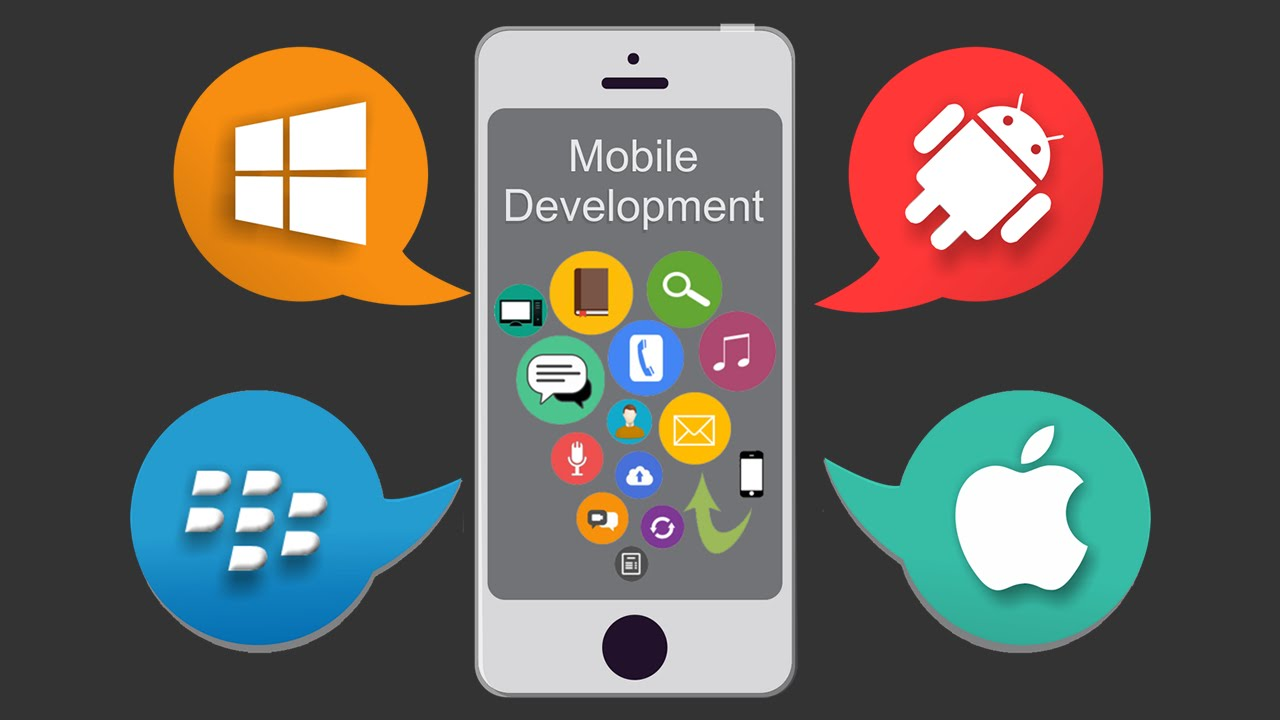
\includegraphics[width=0.5\columnwidth]{Figures/2/hybrid}
	\caption{Hybrid Mobile Application คืออะไร}{ที่มา :  https://www.mindphp.com/คู่มือ/73-คืออะไร/3663-hybrid-application-ไฮบริด-แอปพลิเคชัน-หรือ-hybrid-app-ไฮบริด-แอพ-คืออะไร.html}
	\label{Fig:hybrid}
\end{figure}

การพัฒนา Mobile Application แต่เดิมนั้น ถ้าจะเริ่มก็คงตั้งแต่ยุค J2ME อาจจะเก่ามากจนมาถึงยุคสมัยของ IOS และ Android 
รวมไปถึงน้องสุดท้องอย่าง Windows Phone 
ซึ่งแต่ก่อนก็มีพัฒนาจาก Window CE มาก่อนหน้านี้ จนผู้ใช้ของแต่ละฝั่ง platform เริ่มมีความสำคัญใกล้เคียงกัน ดังนั้น การพัฒนาแอป
เฉพาะของ iOS หรือ Android เพียงอย่างเดียวถือเป็นการเสียโอกาสทางธุรกิจเป็นอย่างมาก จนมีคนเริ่มคิดหาวิธีทำให้ชีวิตง่ายขึ้นโดยการเขียน 
HTML5 + CSS3 + JavaScript แล้วใช้วิธีทำงานผ่าน Web View Component เป็นส่วนของหน้าเบราเซอร์ในแอปอีกที ของแต่ละ Platform 
จนกลายมาเป็นโครงการ Cordova และได้มีการพัฒนาส่วนขยาย Plug-In เพิ่มเรื่อยๆ ทำให้ปัจจุบันเราสามารถเข้าถึง Hardware หรือ Sensor 
ซึ่งโดยปกติ HTML5 ธรรมดาไม่สามารถเข้าถึงได้ 

\begin{figure}[H]
	\centering
	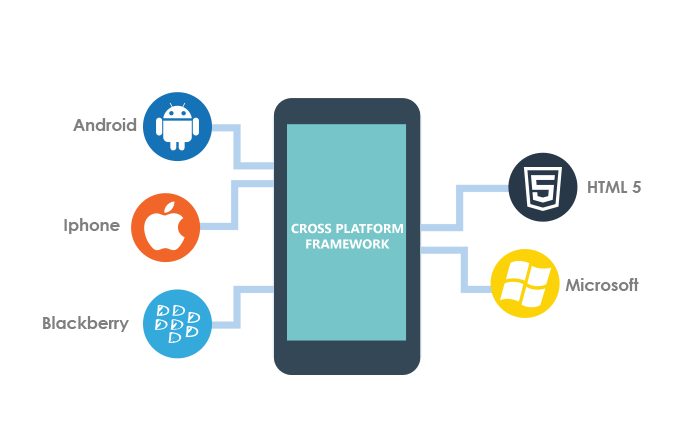
\includegraphics[width=0.5\columnwidth]{Figures/2/hybrid2}
	\caption{Cross Platform Frameworks}{ที่มา :  https://www.promaticsindia.com/mobile-app-development-services/cross-platform-frameworks}
	\label{Fig:hybrid2}
\end{figure}

การเขียนแอปแบบ Hybrid Application คือ การพัฒนาโดยอาศัย Framwork หรือ SDK 
ที่ถูกสร้างมาจากหลากหลายภาษาและมีเครื่องมือที่เหมาะสมกับ Framwork หรือ SDK นั้น ๆ ให้เลือกใช้ในการพัฒนาที่หลากหลายตัวอย่างเช่น 
codova SDK ใช้ ภาษา LUA , Acrobat AIR ใช้ภาษา ACTION SCRIPT 3 หรือ UNITY ใช้ C# และ JAVASCRIPT 
ซึ่งการเขียนในรูปแบบนี้เราสามารถแปลงไปใช้กับระบบปฏิบัติการอื่น ๆ ได้และใช้เวลาน้อยในการเพื่อพัฒนาหลาย ๆ แอปพลิเคชัน

	ข้อดีของ Hybrid Mobile Application
	\begin{enumerate}[label=\arabic*)]
		\item พัฒนาด้วยภาษา HTML, CSS และ JavaScript ทำให้ง่ายและเรียนรู้ได้อย่างรวดเร็ว
		\item พัฒนาครั้งเดียวสามารถใช้ได้หลาย Platform ทั้ง iOS, Android และ Window Phone
		\item ใช้ต้นทุนในการพัฒนาน้อยกว่า Native App
	\end{enumerate}

	ข้อเสียของ Hybrid Mobile Application
	\begin{enumerate}[label=\arabic*)]
		\item ประสิทธิภาพการทำงานจะด้อยกว่า Native App
		\item ในบางกรณีอาจจะใช้ความสามารถของอุปกรณ์ได้ไม่เต็มที่ เนื่องจากต้องขึ้นอยู่กับ Framework ที่เลือกในการพัฒนานั้นมี Component ที่ต้องการหรือไม่
		ดังนั้น Hybrid App จึงมีจุดเด่นในเรื่องความง่ายและพัฒนาได้รวดเร็ว และ Cross-Platforms คือพัฒนาครั้งเดียวแต่สามารถนำไปติดตั้งในหลาย Platforms แต่เมื่อพูดถึงเรื่องประสิทธิภาพในการทำงาน เช่นความเร็ว หรือการเรียกใช้หรือติดต่อ feature ต่าง ๆ ของอุปกรณ์ ก็ต้องยอมรับว่าอาจจะยังด้อยกว่าแอปพลิเคชันที่พัฒนาด้วย Native App ในบางลักษณะการทำงานอยู่ดี
	\end{enumerate}

% Android Studio

\subsection{ความรู้พื้นฐานระบบปฏิบัติการแอนดรอยด์}
แอนดรอยด์ (Android) คือระบบปฏิบัติการแบบเปิดเผยซอร์ฟแวร์ต้นฉบับ (Open Source) โดยบริษัท กูเกิ้ล (Google Inc.) ที่ได้รับความนิยมเป็นอย่างสูง เนื่องจากอุปกรณ์ที่ใช้ระบบปฏิบัติการแอนดรอยด์ มีจำนวนมาก อุปกรณ์มีหลากหลายระดับ หลายราคา รวมทั้งสามารถทำงานบนอุปกรณ์ที่มีขนาดหน้าจอ และความละเอียดแตกต่างกันได้ ทำให้ผู้บริโภคสามารถเลือกได้ตามต้องการและหากมองในทิศทางสำหรับนักพัฒนาโปรแกรม (Programmer) แล้วนั้นการพัฒนาโปรแกรมเพื่อใช้งานบนระบบปฏิบัติการแอนดรอยด์ ไม่ใช่เรื่องยาก เพราะมีข้อมูลในการพัฒนารวมทั้ง Android SDK (Software Development Kit) เตรียมไว้ให้กับนักพัฒนาได้เรียนรู้ และเมื่อนักพัฒนาต้องการจะเผยแพร่หรือจำหน่ายโปรแกรมที่พัฒนาแล้วเสร็จแอนดรอยด์ก็ยังมีตลาดในการเผยแพร่โปรแกรม Google PlayStore แต่หากจะกล่าวถึงโครงสร้างภาษาที่ใช้ในการพัฒนานั้น สำหรับ Android SDK จะยึดโครงสร้างของภาษาจาวา (Java language) ในการเขียนโปรแกรม เพราะโปรแกรมที่พัฒนามาได้จะต้องทำงานอยู่ภายใต้ Dalvik Virtual Machine เช่นเดียวกับโปรแกรมจาวา ที่ต้องทำงานอยู่ภายใต้ Java Virtual Machine (Virtual Machine เปรียบได้กับสภาพแวดล้อมที่โปรแกรมทำงานอยู่)

	\subsubsection{โครงสร้างของระบบปฏิบัติการแอนดรอยด์} 
	การทำความเข้าใจโครงสร้างของระบบปฏิบัติการแอนดรอยด์ \cite{androidbook1} ถือว่าเป็นสิ่งสำคัญเพราะถ้านักพัฒนาโปรแกรม สามารถมองภาพโดยรวมของระบบได้ทั้งหมด จะสามารถเข้าใจถึงกระบวนการทำงานได้ดียิ่งขึ้น และสามารถนำไปช่วยในการออกแบบโปรแกรมที่ต้องการพัฒนาเพื่อให้เกิดประสิทธิภาพในการทำงาน
	
	\begin{figure}[H]
		\centering
		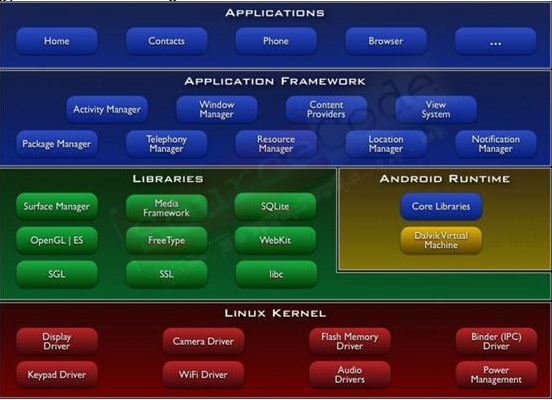
\includegraphics[width=0.8\columnwidth]{Figures/2/androidarchitecture}
		\caption{โครงสร้างของระบบปฏิบัติการแอนดรอยด์}{ที่มา : https://www.theandroid-mania.com/android-architecture/}
		\label{Fig:androidarchitecture}
	\end{figure}
	จากโครงสร้างของระบบปฏิบัติการแอนดรอยด์ในรูปที่ \ref{Fig:androidarchitecture} จะสังเกตได้ว่า มีการแบ่งออกเป็นส่วน ๆ ที่มีความเกี่ยวเนื่องกัน โดยส่วนบนสุดเป็นส่วนที่ผู้ใช้งานทำการติดต่อโดยตรงซึ่งคือส่วนของ Applications ลำดับถัดมาเป็นองค์ประกอบอื่น ๆ ตามลำดับ และสุดท้ายเป็นส่วนที่ติดต่อกับอุปกรณ์โดยผ่านทาง Linux Kernel โครงสร้างของแอนดรอยด์สามารถอธิบายได้ดังนี้

	\begin{enumerate}[label=\arabic*)]
		\item Applications ส่วนแอปพลิเคชันหรือส่วนของโปรแกรมที่มากับระบบปฏิบัติการ หรือเป็นกลุ่มของโปรแกรมที่ผู้ใช้งานได้ทำการติดตั้งไว้ โดยผู้ใช้งานสามารถเรียกใช้โปรแกรมต่าง ๆ ได้โดยตรงซึ่งการทำงานของแต่ละโปรแกรมจะเป็นไปตามที่ผู้พัฒนาโปรแกรมได้ออกแบบและเขียนโค้ด (Code) โปรแกรมเอาไว้
		\item Application Framework  เป็นส่วนที่มีการพัฒนาขึ้นเพื่อให้นักพัฒนาสามารถพัฒนาโปรแกรมได้สะดวก และมีประสิทธิภาพมากยิ่งขึ้น โดยนักพัฒนาไม่จำเป็นต้องพัฒนาในส่วนที่มีความยุ่งยากมากๆ เพียงแค่ทำการศึกษาถึงวิธีการเรียกใช้งาน Application Framework ในส่วนที่ต้องการใช้งานแล้วนำมาใช้งาน ซึ่งมีหลายกลุ่มด้วยกัน ตัวอย่างเช่น
			\begin{itemize}
				\item Activities Manager เป็นกลุ่มของชุดคำสั่งที่จัดการเกี่ยวกับวงจรการทำงานของหน้าต่างโปรแกรม (Activity)
				\item Content Providers เป็นกลุ่มของชุดคำสั่ง ที่ใช้ในการเข้าถึงข้อมูลของโปรแกรมอื่น และสามารถแบ่งปันข้อมูลให้โปรแกรมอื่นเข้าถึงได้
				\item View System เป็นกลุ่มของชุดคำสั่งที่เกี่ยวกับการจัดการโครงสร้างของหน้าจอที่แสดงผลในส่วนที่ติดต่อกับผู้ใช้งาน (User Interface)
				\item Telephony Manager เป็นกลุ่มของชุดคำสั่งที่ใช้ในการเข้าถึงข้อมูลด้านโทรศัพท์ เช่น หมายเลขโทรศัพท์ เป็นต้น
				\item Resource Manager เป็นกลุ่มของชุดคำสั่งในการเข้าถึงข้อมูลที่เป็นข้อความและรูปภาพ
				\item Location Manager เป็นกลุ่มของชุดคำสั่งที่เกี่ยวกับตำแหน่งทางภูมิศาสตร์ที่ระบบปฏิบัติการได้รับค่าจากอุปกรณ์
				\item Notification Manager เป็นกลุ่มของชุดคำสั่งที่จะถูกเรียกใช้เมื่อโปรแกรมต้องการแสดงผลให้กับผู้ใช้งาน ผ่านทางแถบสถานะ (Status Bar) ของหน้าจอ
			\end{itemize}
		\item Libraries เป็นส่วนของชุดคำสั่งที่พัฒนาด้วย C/C++ โดยแบ่งชุดคำสั่งออกเป็นกลุ่มตามวัตถุประสงค์ของการใช้งาน เช่น Surface Manage จัดการเกี่ยวกับการแสดงผล Media Framework จัดการเกี่ยวกับการการแสดงภาพและเสียง Open GL|ES และ SGL จัดการเกี่ยวกับภาพ 3 มิติ และ 2 มิติ SQLlite จัดการเกี่ยวกับระบบฐานข้อมูล เป็นต้น
		\item Android Runtime จะมี Darvik Virtual Machine ที่ถูกออกแบบมาเพื่อให้ทำงานบนอุปกรณ์ที่มีหน่วยความจำ (Memmory) หน่วยประมวลผลกลาง (CPU) และพลังงาน (Battery) ที่จำกัดซึ่งการทำงานของ Darvik Virtual Machine จะทำการแปลงไฟล์ที่ต้องการทำงานไปเป็นไฟล์ .DEX ก่อนการทำงานเหตุผลเพื่อให้มีประสิทธิภาพเพิ่มขึ้นเมื่อใช้งานกับหน่วยประมวลผลกลางที่มีความเร็วไม่มากส่วนต่อมาคือ Core Libraries ที่เป็นส่วนรวบรวมคำสั่งและชุดคำสั่งสำคัญโดยถูกเขียนด้วยภาษาจาวา (Java Language)
		\item Linux Kernel เป็นส่วนที่ทำหน้าที่หัวใจสำคัญในจัดการกับบริการหลักของระบบปฏิบัติการ เช่น เรื่องหน่วยความจำ พลังงาน ติดต่อกับอุปกรณ์ต่างๆ ความปลอดภัย เครือข่าย โดยแอนดรอยด์ได้นำเอาส่วนนี้มาจากระบบปฏิบัติการลินุกซ์ รุ่น 2.6 (Linux 26. Kernel) ซึ่งได้มีการออกแบบมาเป็นอย่างดี
	\end{enumerate}

	\subsubsection{ข้อเด่นของระบบปฏิบัติการแอนดรอยด์} 
	เนื่องจากระบบปฏิบัติการแอนดรอยด์มีการเจริญเติบโตอย่างรวดเร็วและมีส่วนแบ่งตลาดของอุปกรณ์ด้านนี้ขึ้นทุกขณะ ทำให้กลุ่มผู้ใช้งานและกลุ่มนักพัฒนาโปรแกรมให้ความสำคัญกับระบบปฏิบัติการแอนดรอยด์เพิ่มมากขึ้น
	เมื่อมองในด้านของกลุ่มผลิตภัณฑ์บริษัทที่มีการพัฒนาผลิตภัณฑ์รุ่นใหม่ ได้มีการนำเอาระบบปฏิบัติการแอนดรอยด์ไปใช้ในสินค้าของตนเองพร้อมทั้งยังมีการปรับแต่งให้ระบบปฏิบัติการมีความสามารถ การจัดวาง โปรแกรมและลูกเล่นใหม่ ๆ ที่แตกต่างจากคู่แข่งในท้องตลาดโดยเฉพาะอย่างยิ่งกลุ่มสินค้าที่เป็นมือถือรุ่นใหม่(SmartPhone)และอุปกรณ์จอสัมผัส(Touch Screen)โดยมีลักษณะแตกต่างกันไป เช่น ขนาดหน้าจอ ระบบโทรศัพท์ ความเร็วของหน่วยประมวลผล ปริมาณหน่วยความจำ แม้กระทั่งอุปกรณ์ตรวจจับ(Sensor)ต่าง ๆ 
	หากมองในด้านของการพัฒนาโปรแกรม ทางบริษัท Google ได้มีการพัฒนา Application Framework ไว้สำหรับนักพัฒนาใช้งานได้อย่างสะดวกและไม่เกิดปัญหาเมื่อนำชุดโปรแกรมที่พัฒนาขึ้นมา ไปใช้กับอุปกรณ์ที่มีลักษณะต่างกัน เช่น ขนาดจออุปกรณ์ไม่เท่ากัน ก็ยังสามารถใช้งานโปรแกรมได้เหมือนกัน เป็นต้น

	\subsubsection{การจัดการเกี่ยวกับวัฏจักรแอคทิวิตี้ของแอปพลิเคชัน} 
	ขณะที่ผู้ใช้เปิดใช้งานแอปพลิเคชัน -> ออกจากแอปพลิเคชัน -> แล้วก็กลับเข้ามาในแอปพลิเคชันอีกครั้งแอคทิวิตี้จะมีการย้าย Method ต่างๆ เกิดขึ้นในวัฏจักรแอคทิวิตี้ ยกตัวอย่างเช่น 
	เมื่อแอคทิวิตี้เริ่มทำงานครั้งแรกจะแสดงขึ้นมาอยู่ด้านบนสุดของระบบ (Foreground) และรอรับการทำงานจากผู้ใช้ในระหว่างกระบวนการนี้ระบบจะมีการเรียกใช้งาน Callback Method หรือ Method ที่ถูกเรียกใช้งานอัตโนมัติในแอคทิวิตี้ที่ได้กำหนดการทำงานให้กับ UI และสวนติดต่ออื่น ๆ ไว้ ถ้าผู้ใช้มีการใช้งานใด ๆ ที่เป็นการเรียกแอคทิวิตี้อื่นขึ้นมาหรือสลับไปใช้งานแอปพลิเคชันอื่นระบบจะเรียก Callback Method อีกอันขึ้นมา เช่น ซ่อนแอปพลิเคชันไว้ด้านหลัง Background (ไม่แสดงแอคทิวิตี้แต่ Instance และ Method นั้นยังทำงานอยู่)
	
	ภายใน Callback Method สามารถกำหนดการทำงานในแอคทิวิตี้เมื่อผู้ใช้ออกจากแอปพลิเคชันและกลับเข้ามาใช้งานแอปพลิเคชันใหม่อีกครั้งได้ ตัวอย่าง ถ้าแอปพลิเคชันเป็นแอปพลิเคชัน Streaming Video
	อาจจะสั่งให้ทำการหยุด Video ชั่วคราว และปิดการเชื่อมต่อ Network ไว้ก่อนเมื่อผู้ใช้สลับไปใช้แอปพลิเคชันอื่น
	และทันทีที่ผู้ใช้กลับมาใช้งานแอปพลิเคชันต่อ ก็ให้ทำการเชื่อมต่อกับ Network และก็อนุญาตให้ผู้ใช้กลับไปเล่น Video
	ในตำแหน่งที่ค้างต่อไปทันทีได้โดยที่ไม่ต้องเริ่มต้นแอปพลิเคชันใหม่ เป็นต้น
	
	\subsubsection{กระบวนการเริ่มทำงานของแอคทิวิตี้ (Activity)} 
	ในระบบแอนดรอย์การกำหนดโค้ดเริ่มต้นไว้ในแอคทิวิตี้โดยสัมพันธ์กับ Method ที่ถูกเรียกใช้งานอัตโนมัติ (Callback Method) อย่างเป็นลำดับ ตั้งแต่เริ่มต้นแอคทิวิตี้ไปจนถึงสิ้นสุดและปิดการทำงานของ Activity ลง

	ในขณะที่แอคทิวิตี้ \cite{ActivityLifeCycle} ทำงานระบบจะเรียกใช้ Callback Method ตามลำดับในลักษณะที่คล้ายกับการก่อพีระมิด นั่นคือ แต่ละขั้นตอนวัฏจักรของแอคทิวิตี้คือส่วนแยกย่อยแต่ละขั้นของพีระมิด
	เช่น เมื่อระบบสร้าง Instance ของแอคทิวิตี้ขึ้นมาใหม่ Method ที่เรียกใช้งานอัตโนมัติ (Callback Method) จะขยับ Activity Method ขึ้นมาด้านบนโดยด้านบนของพีระมิดคือจุดที่แอคทิวิตี้กำลังทำงานแสดงอยู่ด้านหน้า (Foreground Activity) สุดและผู้ใช้กำลังใช้งานอยู่และเมื่อผู้ใช้กำลังจะออกจากแอคทิวิตี้ระบบจะเรียกใช้ Method อื่นซึ่งทำให้ Activity Method
	ถอยกลับไปอยู่ด้านล่างของพีระมิดตามลำดับเพื่อหยุดการทำงานและลบแอคทิวิตี้ออกไป ในบางกรณีแอคทิวิตี้จะย้ายลงมาอยู่บางจุดและรอจังหวะที่จะถูกเรียกกลับขึ้นมาด้านบนอีก เช่น ในกรณีเมื่อผู้ใช้สลับไปใช้งานแอปพลิเคชันอื่นแล้วกลับมาใช้งานอีกครั้ง
	
	\begin{figure}[H]
		\centering
		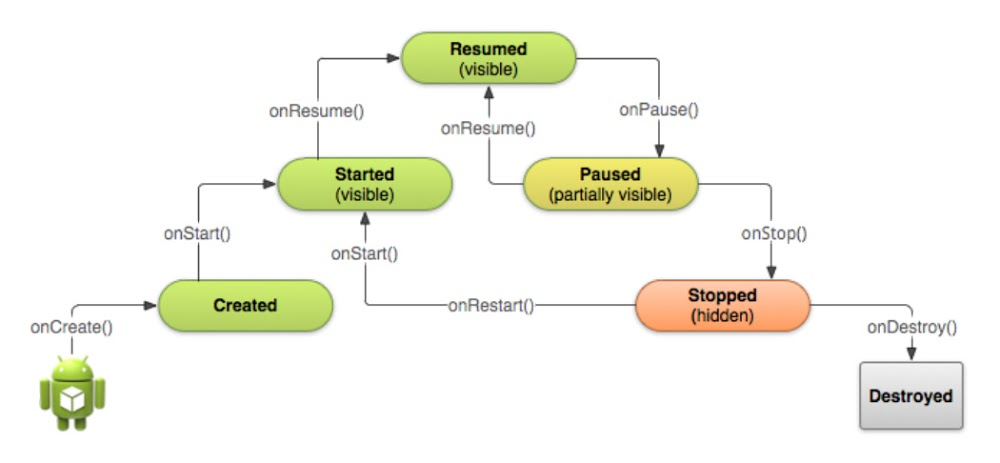
\includegraphics[width=0.8\columnwidth]{Figures/2/lifecycle}
		\caption{วัฏจักรของแอคทิวิตี้บนระบบปฏิบัติการแอนดรอยด์}{ที่มา : https://www.dev2qa.com/android-activity-lifecycle-example/}
		\label{Fig:lifecycle}
	\end{figure}

	จากรูปที่ \ref{Fig:lifecycle} แสดงวัฏจักรของแอคทิวิตี้ในรูปแบบโครงสร้างพีระมิดโดยแสดงให้เห็นว่า Method ที่เรียกใช้
	งานอัตโมัติ (Callback Method) ได้แก่ onCreate(), onStart(), onResume() และ onRestart() จะขยับแอคทิวิตี้ขึ้นไปด้านบนสุดที่ Resumed Method
	และมี Method ได้แก่ onPause(), onStop() และ onDestroy() ที่จะขยับแอคทิวิตี้ลงมาด้านล่าง แอคทิวิตี้ยังสามารถกลับไปทำงานที่ตำแหน่ง Resumed Method จากตำแหน่ง Paused และ Stopped ได้อีกด้วย
	
	ในบางครั้งไม่จำเป็นต้องเรียกใช้งาน Callback Method ทั้งหมดเสมอไปขึ้นกับความซับซ้อนของแอคทิวิตี้ อย่างไรก็ตามเป็นสิ่งสำคัญที่นักพัฒนาควรทำความเข้าใจแต่ละ Method เพื่อให้มั่นใจได้ว่าแอปพลิเคชันของที่ได้พัฒนาตอบสนองเป็นไปตามที่ผู้ใช้คาดหวัง ดังนั้น ในการใช้งาน Callback Method
	ที่ถูกวิธีก็จะช่วยให้แอปพลิเคชันทำงานได้เป็นอย่างดี ดังนี้
	\begin{itemize}
		\item ไม่หยุดการทำงานหรือค้าง กรณีมีสายโทรเข้าหรือมีการสลับไปใช้งานแอปพลิเคชันอื่น 
		\item ไม่ใช้ทรัพยากรที่มีค่าของระบบอย่างสูญเปล่า ถ้าไม่มีการใช้งานแอคทิวิตี้ใดๆ 
		\item ไม่กระทบต่อกระบวนการในขั้นตอนการใช้งานของผู้ใช้กรณีออกจากแอปพลิเคชันแล้วกลับเข้ามาใช้งานอีกครั้ง 
		\item ไม่หยุดการทำงานหรือระบบค้างที่กระทบการใช้งานของผู้ใช้กรณีมีการหมุนหน้าจอแนวนอนและแนวตั้งสลับกัน
	\end{itemize}
	
	เหตุการณ์ที่แอคทิวิตี้มีการเปลี่ยน Method ต่าง ๆ ตามแสดงในรูปที่  \ref{Fig:lifecycle}
	แต่มีอยู่ 3 Method เท่านั้นที่แอคทิวิตี้จะยังคงอยู่คงที่ในช่วงเวลาระยะเวลาหนึ่งไม่เปลี่ยนไป Method อื่นในทันที ได้แก่
		\begin{itemize}
		\item Resumed (แสดงอยู่ ทำงานอยู่) ใน Method นี้แอคทิวิตี้จะแสดงอยู่ด้านหน้าสุดและผู้ใช้กำลังใช้งานอยู่ บ่อยครั้งจะเรียกว่า Running Method
		\item Paused (แสดงหน้าจอบางส่วน ไม่ถูกบังสนิท) ใน Method นี้แอคทิวิตี้จะถูกบดบังด้วยแอคทิวิตี้อื่น เช่น แอคทิวิตี้อื่นที่อยู่ด้านหน้าสุดที่แสดงในลักษณะกึ่งโปรงใสหรือไม่ได้แสดงแบบเต็มหน้าจอ  แอคทิวิตี้ในสถานะนี้จะไม่สามารถรับค่าจากผู้ใช้และทำงานคำสั่งใด ๆ ได้
		\item Stopped (แสดงหน้าจอแบบ Background ผู้ใช้มองไม่เห็น) ใน Method นี้ แอคทิวิตี้จะถูกบดบังอย่างสมบูรณ์และผู้ใช้มองไม่เห็นโดยจะถูกย้ายไปอยู่ด้านหลังในขณะที่อยู่ใน Method นี้
		ค่า Activity Instance และตัวแปรทั้งหมดจะยังคงอยู่แต่จะไม่สามารถถูกเรียกมาใช้งานจากโค้ดใด ๆ ได้
		\end{itemize}

		ในขณะที่ Method อื่น เช่น Created และ Started จะแสดงชั่วคราวแล้วระบบก็จะเปลี่ยนไป Method อื่นในทันทีที่ Method ถูกเรียกใช้งานอัตโนมัติ นั่นคือ หลังจากที่ระบบเรียกใช้งาน onCreate() แล้วก็จะเรียกใช้งาน onStart() ทันทีและสุดท้ายตามด้วย onResumne()  ซึ่งก็จะเข้าสู่ Resumed Method ทั้งหมดก็คือวัฏจักรแอคทิวิตี้เบื้องต้น

	
% IOS 

	\subsection{ความรู้พื้นฐานระบบปฏิบัติการ iOS}
	ระบบปฏิบัติการไอโอเอส (iOS) \cite{iosref} มีชื่อเดิมว่า iPhone OS เริ่มต้นด้วยการเปิดตัวของ iPhone เมื่อวันที่ 29 มิถุนายน 2550 ระบบปฏิบัติการไอโอเอส (iOS) เป็นระบบปฏิบัติการสำหรับสมาร์ทโฟน (Smartphone) ของแอปเปิล โดยเริ่มต้นพัฒนาสำหรับใช้ในโทรศัพท์ iPhone และได้พัฒนาต่อใช้สำหรับ iPot Touch และiPad โดยระบบปฏิบัติการนี้สามารถเชื่อมต่อไปยังแอ็ปสตอร์สำหรับการเข้าถึงถึงแอพพลิเคชั่น(Application) มากกว่า 300,000 ตัว ซึ่งมีการดาวน์โหลดไปมากกว่าห้าพันล้านครั้ง แอปเปิลได้มีการพัฒนาปรับปรุงสำหรับ iPhone, iPad และ iPod Touch ผ่านทางระบบ iTunes คือโปรแกรมฟรี สำหรับ Mac และ PC ใช้ดูหนังฟังเพลงบนคอมพิวเตอร์ รวมทั้งจัดระเบียบและ sync ทุกๆอย่าง และเป็นร้านขายความบันเทิงบนคอมพิวเตอร์, บน iPod touch, iPhone และ iPad ที่มีทุกๆอย่างสำหรับคุณ ในทุกที่และทุกเวลา พัฒนาระบบรักษาความปลอดภัยให้มีความเป็นเลิศ ซึ่งนี้คือข้อได้เปรียบ เมื่อเทียบกับคู่แข่ง	

	\subsubsection{เวอร์ชันของ iOS} 
	iOS 1 (iPhone OS)

	สำหรับ iOS 1 ถูกเปิดตัวครั้งแรกที่งาน Macworld วันที่ 9 มกราคม 2007 พร้อมกับ iPhone รุ่นแรก และหลังจากนั้นก็ออกวางจำหน่ายพร้อม iPhone วันที่ 29 มิถุนายน 2007 สำหรับ iOS 1 มาพร้อมฟีเจอร์เด่น ๆ เช่น ระบบสัมผัสแบบมัลติทัช, voicemail, ท่องเว็บผ่าน Safari และดู YouTube แต่ iOS 1 ไม่ได้ฟรีสำหรับผู้ใช้งาน iPod touch จะต้องจ่ายเงิน 19.99 เหรียญ หรือประมาณ 690 บาท เพื่ออัปเดตเป็น iOS 1

	\begin{figure}[H]
		\centering
		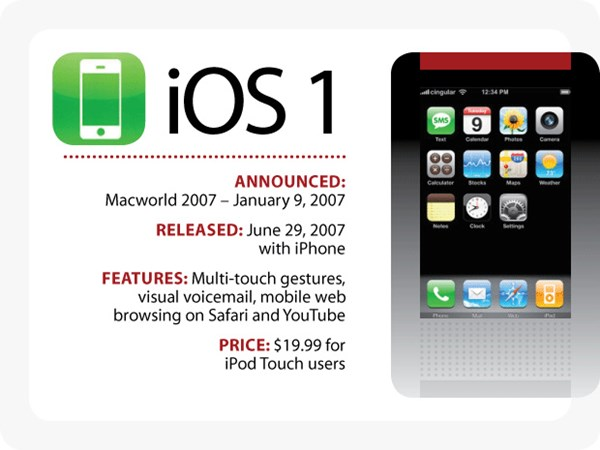
\includegraphics[width=0.8\columnwidth]{Figures/2/iOS/iOS1}
		\caption{iOS 1}{ที่มา : https://mobile.kapook.com/view5432.html}
		\label{Fig:iosversion1}
	\end{figure}

	iOS 2 (iPhone OS 2.0)

	เปิดตัวครั้งแรกที่งาน WWDC 2008 (วันที่ 9 มิถุนายน 2008) และหลังจากนั้นก็ออกวางจำหน่ายพร้อม iPhone 3G วันที่ 11 กรกฎาคม 2008 โดยมีฟีเจอร์เด่น ๆ เช่น App Store, แผนที่พร้อม GPS และระบบแจ้งเตือนอีเมล และเหมือนเช่นเคยผู้ใช้ iPhone สามารถอัปเดตได้ฟรี แต่ผู้ใช้ iPod touch จะต้องจ่ายเงิน 9.95 เหรียญ หรือประมาณ 390 บาท เพื่ออัปเดต iOS 2.x

	\begin{figure}[H]
		\centering
		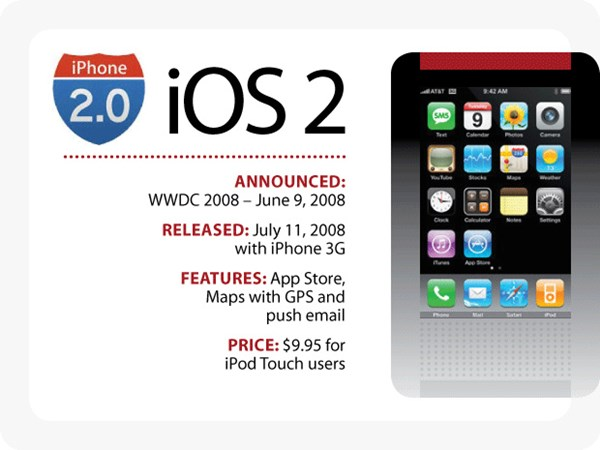
\includegraphics[width=0.8\columnwidth]{Figures/2/iOS/iOS2}
		\caption{iOS 2}{ที่มา : https://mobile.kapook.com/view5432.html}
		\label{Fig:iosversion2}
	\end{figure}

	iOS 3 (iPhone OS 3.0)

	เปิดตัวครั้งแรกที่งาน WWDC 2009 (วันที่ 8 มิถุนายน 2009) และหลังจากนั้นก็ออกวางจำหน่ายพร้อม iPhone 3GS วันที่ 19 มิถุนายน 2009 สำหรับเวอร์ชั่นนี้มาพร้อมฟีเจอร์เด่น ๆ อย่าง Voice Control, สามารถคัดลอกและวางข้อความ และส่ง MMS ได้ เหมือนเช่นเคยผู้ใช้ iPhone สามารถอัปเดตได้ฟรี แต่ผู้ใช้ iPod touch จะต้องจ่ายเงิน 9.95 เหรียญ หรือประมาณ 390 บาท เพื่ออัปเดต iOS 3.0 - 3.1 และ 4.95 เหรียญ หรือประมาณ 169 บาท สำหรับอัปเดต iOS 3.2

	\begin{figure}[H]
		\centering
		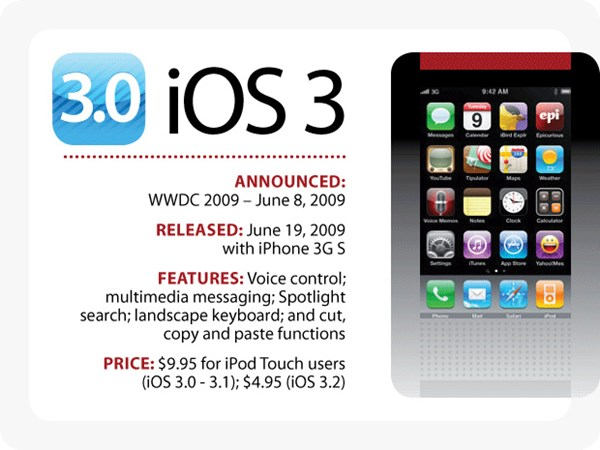
\includegraphics[width=0.8\columnwidth]{Figures/2/iOS/iOS3}
		\caption{iOS 3}{ที่มา : https://mobile.kapook.com/view5432.html}
		\label{Fig:iosversion3}
	\end{figure}

	iOS 4 

	ถือว่าเป็นระบบปฏิบัติการรุ่นแรกของแอปเปิล ที่เปลี่ยนชื่อเรียกจาก iPhone OS มาเป็น iOS โดย iOS 4 เปิดตัวครั้งแรกที่งาน WWDC 2010 (วันที่ 7 มิถุนายน 2010) หลังจากนั้นก็ออกวางจำหน่ายพร้อม iPhone 4 วันที่ 21 มิถุนายน 2010 และมีฟีเจอร์ใหม่ ๆ ที่น่าสนใจมากมาย เช่น Multitasking, โฟลเดอร์, FaceTime, iBook และ iOS 4.2.1 เป็นรุ่นแรกรองรับการใช้งานบน iPad มาถึงเวอร์ชั่นนี้ทุกอุปกรณ์ iOS ของแอปเปิล สามารถอัปเดตได้ฟรี

	\begin{figure}[H]
		\centering
		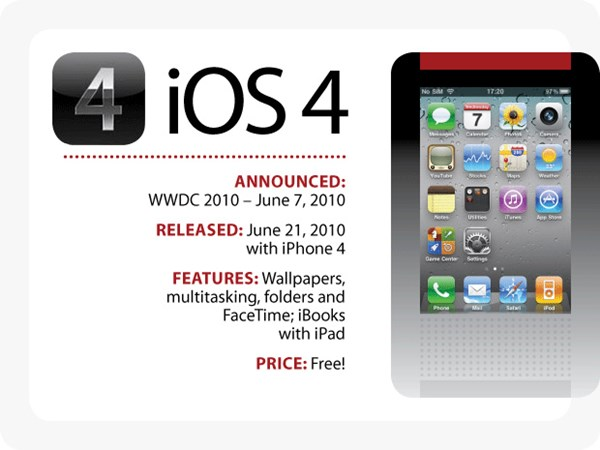
\includegraphics[width=0.8\columnwidth]{Figures/2/iOS/iOS4}
		\caption{iOS 4}{ที่มา : https://mobile.kapook.com/view5432.html}
		\label{Fig:iosversion4}
	\end{figure}

	iOS 5 

	เปิดตัวพร้อม iPhone 4S ที่งาน WWDC 2011 (วันที่ 6 มิถุนายน 2011) และหลังจากนั้นก็ออกวางจำหน่ายพร้อม iPhone 4S วันที่ 12 ตุลาคม 2011 มาพร้อมฟีเจอร์ใหม่ที่น่าสนใจหลายอย่าง เช่น Siri, iCloud, Notification Center, iMessage, Reminders และ Newsstand เป็นต้น

	\begin{figure}[H]
		\centering
		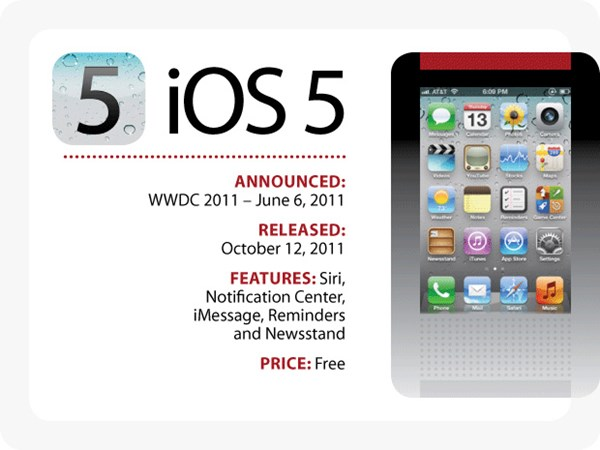
\includegraphics[width=0.8\columnwidth]{Figures/2/iOS/iOS5}
		\caption{iOS 5}{ที่มา : https://mobile.kapook.com/view5432.html}
		\label{Fig:iosversion5}
	\end{figure}

	iOS 6 

	เปิดตัวพร้อม iPhone 5 และ iPad mini ที่งาน WWDC 2012 (วันที่ 11 มิถุนายน 2012) และออกวางจำหน่ายพร้อม iPhone 5 วันที่ 19 กันยายน 2012 สำหรับฟีเจอร์ใหม่ที่มาพร้อม iOS 6 เช่น การเปลี่ยนไปใช้ระบบแผนที่ของแอปเปิลเอง, สามารถ Facetime ผ่านระบบเซลลูลาร์, ถ่ายภาพแบบพาโนรามา, คีย์บอร์ดภาษาไทยแบบ 4 แถว, Passbook, อินทิเกรท Facebook, รองรับ LTE และแอปฯ นาฬิกาสำหรับ iPad

	\begin{figure}[H]
		\centering
		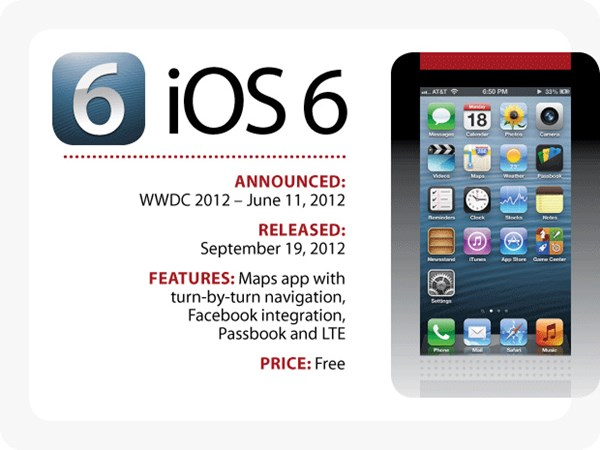
\includegraphics[width=0.8\columnwidth]{Figures/2/iOS/iOS6}
		\caption{iOS 6}{ที่มา : https://mobile.kapook.com/view5432.html}
		\label{Fig:iosversion6}
	\end{figure}

	iOS 7 

	อีกก้าวสำคัญของแอปเปิล ที่มีการยกเครื่องเปลี่ยนดีไซน์ของ iOS ใหม่ทั้งหมด เปิดตัวครั้งแรกที่งาน WWDC 2013 (วันที่ 10 มิถุนายน 2013) และปล่อยให้อัปเดตวันที่ 18 กันยายน 2013 โดยผู้ที่รับหน้าที่ดูแลการปรับโฉม iOS 7 ครั้งนี้ ก็คือ Jonathan Ive เปลี่ยนมาใช้ดีไซน์แบบ Flat Design, ไอคอนใหม่ทั้งหมด, มี Control Center, AirDrop, Photos, iTunes Radio และ CarPlay

	\begin{figure}[H]
		\centering
		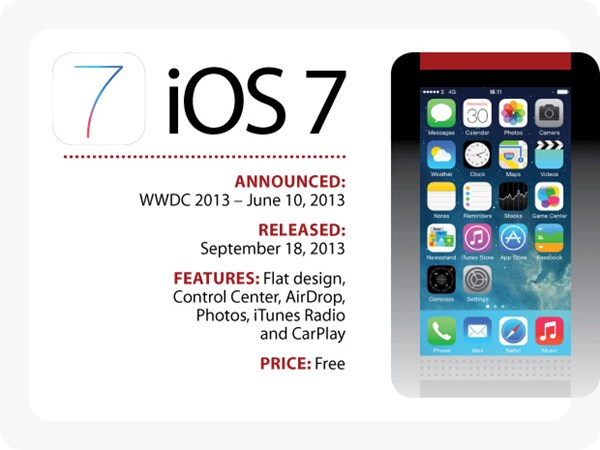
\includegraphics[width=0.8\columnwidth]{Figures/2/iOS/iOS7}
		\caption{iOS 7}{ที่มา : https://mobile.kapook.com/view5432.html}
		\label{Fig:iosversion7}
	\end{figure}

	iOS 8 

	สำหรับ iOS 8 เปิดตัวครั้งแรกที่งาน WWDC 2014 (วันที่ 2 มิถุนายน 2014) และปล่อยให้อัปเดตวันที่ 17 กันยายน 2014 พร้อมการเปิดตัว iPhone 6, 6 Plus และ iPad Air 2 โดยหน้าตาต่าง ๆ ของ iOS 8 ยังคงเหมือนกับ iOS 7 แต่ปรับปรุงประสิทธิภาพการทำงานให้ดีขึ้นกว่าเดิม รวมถึงเพิ่มฟีเจอร์การใช้งานต่าง ๆ เข้ามาอีกอย่างมากมาย เช่น iCloud Drive, Apple Pay, Apple Music, QuickType, Family Sharing และแอปฯ Health เป็นต้น

	\begin{figure}[H]
		\centering
		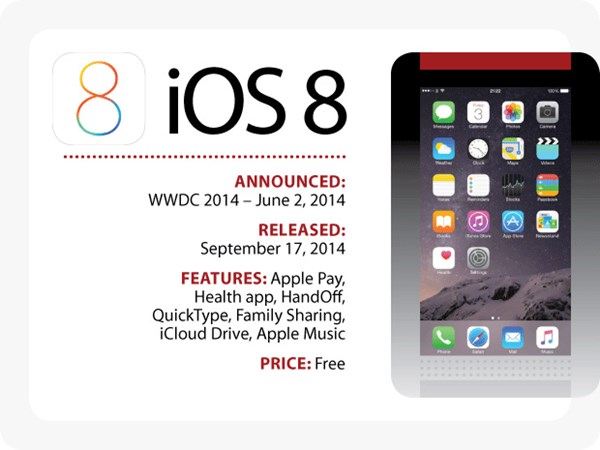
\includegraphics[width=0.8\columnwidth]{Figures/2/iOS/iOS8}
		\caption{iOS 8}{ที่มา : https://mobile.kapook.com/view5432.html}
		\label{Fig:iosversion8}
	\end{figure}

	iOS 9 

	เปิดตัวครั้งแรกที่งาน WWDC 2015 (วันที่ 8 มิถุนายน 2015) และปล่อยให้อัปเดตวันที่ 16 กันยายน 2015 สำหรับเวอร์ชั่นนี้เน้นปรับปรุงเพิ่มประสิทธิภาพการใช้งานให้ดีขึ้นกว่าเดิม รวมถึงเปลี่ยนแปลงและเพิ่มฟีเจอร์ใหม่ที่ช่วยให้ผู้ใช้สะดวกสบายมากขึ้น โดยฟีเจอร์หลาย ๆ อย่างเรียนรู้จากพฤติกรรมผู้ใช้งาน เพื่อตอบสนองสิ่งที่ผู้ใช้งานต้องการมากที่สุด โดยฟีเจอร์ใหม่ที่มาพร้อม iOS 9 เช่น Siri มีความแม่นยำและทำงานได้รวดเร็วกว่าเดิม, รองรับการใช้งาน 2 หน้าจอสำหรับ iPad, เพิ่มแอปฯ News, ปรับปรุงแอปฯ Note, Spotlight ให้สามารถค้นหาสิ่งต่าง ๆ ได้มากขึ้น

	\begin{figure}[H]
		\centering
		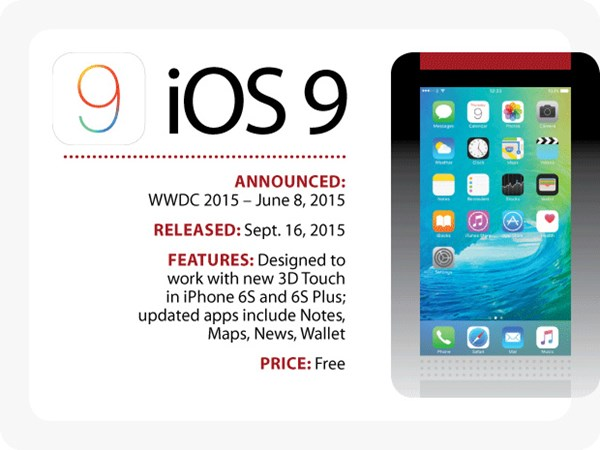
\includegraphics[width=0.8\columnwidth]{Figures/2/iOS/iOS9}
		\caption{iOS 9}{ที่มา : https://mobile.kapook.com/view5432.html}
		\label{Fig:iosversion9}
	\end{figure}

	iOS 10 

	เปิดตัวครั้งแรกที่งาน WWDC 2016 (วันที่ 13 มิถุนายน 2016) และปล่อยให้อัปเดตวันที่ 13 กันยายน 2016 แอปเปิลบอกว่า iOS 10 มาพร้อมการปรับปรุงครั้งใหญ่ ภายในงานได้พูดถึง 10 ฟีเจอร์หลัก ๆ ที่มีการเปลี่ยนแปลงหลาย ๆ อย่าง เช่น อินเทอร์เฟซมีการปรับเปลี่ยนใหม่ให้ดูสวยงามขึ้นกว่าเดิม, ระบบแจ้งเตือนแบบใหม่, 3D Touch ที่ใช้งานได้หลากหลายขึ้น, รีดีไซน์แอปฯ Apple Maps, Apple Music และ News เป็นต้น

	\begin{figure}[H]
		\centering
		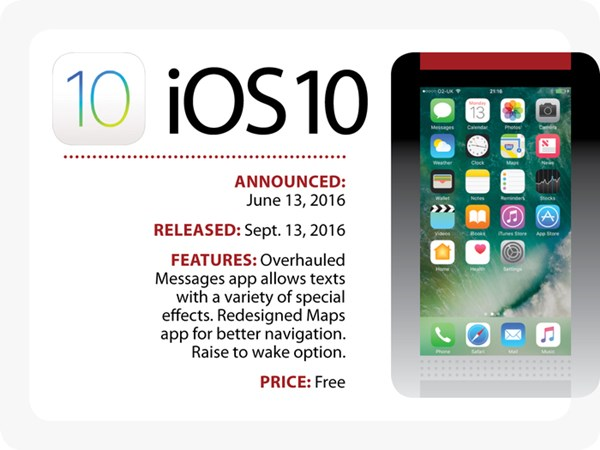
\includegraphics[width=0.8\columnwidth]{Figures/2/iOS/iOS10}
		\caption{iOS 10}{ที่มา : https://mobile.kapook.com/view5432.html}
		\label{Fig:iosversion10}
	\end{figure}

	iOS 11 

	เปิดตัวครั้งแรกที่งาน WWDC 2017 (วันที่ 5 มิถุนายน 2017) และปล่อยให้อัปเดตวันที่ 19 กันยายน 2017 สำหรับเวอร์ชั่นนี้แอปเปิลได้ให้คำนิยามไว้ว่า "เป็นก้าวใหญ่สำหรับ iPhone ก้าวกระโดดสำหรับ iPad" โดยเน้นการปรับปรุงเพิ่มความสามารถรอบด้าน ตอบโจทย์การใช้งานให้ดีขึ้นกว่าเดิม โดยของใหม่ที่มาพร้อม iOS 11 ที่น่าสนใจ เช่น Siri สามารถแปลภาษาได้, ปรับปรุง Control Center ใหม่, Apple Pay รองรับการโอนเงินได้, เพิ่ม API สำหรับระบบ AR เทคโนโลยีที่ผสมผสานระหว่างความเป็นจริงและโลกเสมือน รวมถึงฟีเจอร์ป้องกันการใช้โทรศัพท์ขณะขับรถ

	\begin{figure}[H]
		\centering
		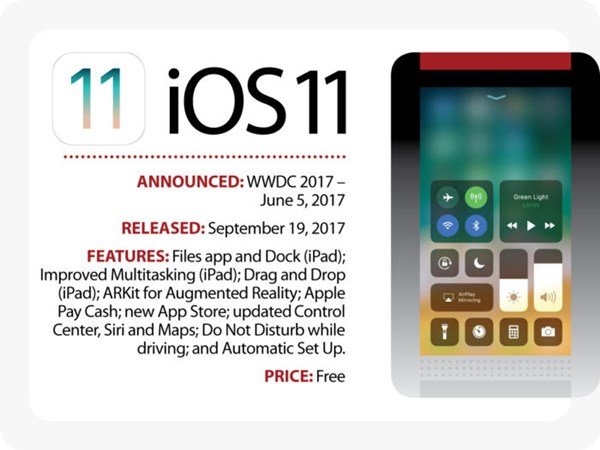
\includegraphics[width=0.8\columnwidth]{Figures/2/iOS/iOS11}
		\caption{iOS 11}{ที่มา : https://mobile.kapook.com/view5432.html}
		\label{Fig:iosversion11}
	\end{figure}
	
	iOS 12 

	เปิดตัวครั้งแรกที่งาน WWDC 2018 (วันที่ 4 มิถุนายน 2018) และจะปล่อยให้อัปเดตในช่วงเดือนกันยายน 2018 หรือหลังจากเปิดตัว iPhone รุ่นใหม่ไปแล้ว สำหรับ iOS 12 ยังคงพัฒนาอย่างต่อเนื่อง โดยออกแบบมาเพื่อทำให้การทำงานประจำวันดำเนินไปอย่างรวดเร็วและตอบสนองฉับไวขึ้น iOS 12 จะเปลี่ยนวิธีการที่ผู้ใช้ iOS มองเห็นโลกโดยใช้ AR ทำให้การสื่อสารมีความสนุกสนานและสื่ออารมณ์ด้วย Memoji, Group FaceTime และ Screen Time ช่วยทำความเข้าใจและจัดการกับเวลาการใช้งานอุปกรณ์ iOS ลดการติดมือถือ นอกจากนี้ยัง iOS 12 เปิดตัว Siri Shortcuts ซึ่งจะทำให้ Siri สามารถทำงานร่วมกับแอปฯ ใดก็ได้

	\begin{figure}[H]
		\centering
		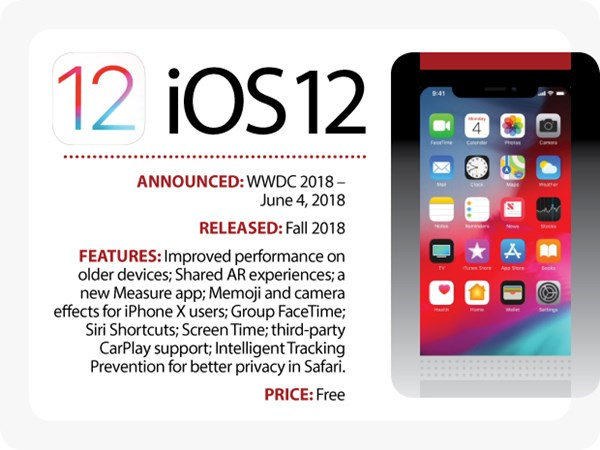
\includegraphics[width=0.8\columnwidth]{Figures/2/iOS/iOS12}
		\caption{iOS 12}{ที่มา : https://mobile.kapook.com/view5432.html}
		\label{Fig:iosversion12}
	\end{figure}

% Ionic Framework

	 \subsection{ความรู้พื้นฐาน Ionic Framework}
	 Ionic Framework \cite{ionicref} คือเครื่องมือในการสร้าง Mobile Application เป็นเครื่องมือสร้างแอปมือถือที่สามารถสร้างทีเดียว สามารถใช้งานได้บนระบบปฏิบัติการ 
	 iOS, Android และ Windows ซึ่งก็จะใช้งานร่วมกับ Framework ตัวอื่น ๆ ได้ คือ Angular และ Apache Cordova 
	 ในตอนสุดท้าย เพื่อให้ทั้งแอปที่เขียนมาใช้ได้กับทุกระบบปฏิบัติการ

		\subsubsection{เทคโนโลยีที่ใช้ในการพัฒนา Ionic Framework} 
		Ionic Framework พัฒนา Frontend ด้วยภาษา HTML , CSS , JavaScript และถูก Build เป็น Application ด้วย Cordova
		\begin{itemize}
		\item HTML5  คือ คือ ภาษามาร์กอัป ที่ใช้สำหรับเขียน website ซึ่ง HTML5 นี้เป็นภาษาที่ถูกพัฒนาต่อมาจากภาษา HTML และพัฒนาขึ้นมาโดย WHATWG (The Web Hypertext Application Technology Working Group) โดยได้มีการปรับเพิ่ม Feature หลายๆอย่างเข้ามาเพื่อให้ผู้พัฒนาสามารถใช้งานได้ง่ายมากยิ่งขึ้น
		\item CSS3  คือ สไตล์ชีท เป็นภาษาที่ใช้เป็นส่วนของการจัดรูปแบบการแสดงผลของ HTML พูดง่ายๆ คือทำให้การแสดงผลของ HTML ให้สวยงาม
		\item AngularJs คือ JavaScript Framework  รูปแบบหนึ่งที่พัฒนามาจาก Google หน้าที่ของมันคือเป็น engine ที่ใช้ควบคุมในส่วน front end ของเว็บได้เป็นอย่างดีมีการทำงานแบบ Model View Controller (MVC)
		\end{itemize}
		\begin{figure}[H]
			\centering
			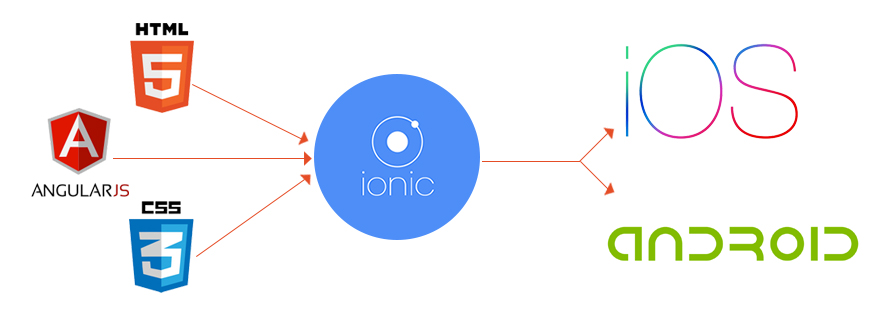
\includegraphics[width=0.8\columnwidth]{Figures/2/ionic1}
			\caption{การทำงานของ Ionic Framework}{ที่มา : http://blog.prscreative.com/what-is-ionic/}
			\label{Fig:ionic}
		\end{figure}

		\subsubsection{การทำงานของ Cordova Application}
		การทำงานของ Hybrid Mobile App คือในช่อง Web App จะมี HTML, CSS, Javascript และไฟล์ภาพ เสียงต่างๆ (Resource) แล้วทำงานผ่าน Web View ที่ PhoneGap จัดเตรียมให้ หากต้องการเข้าถึงส่วนอื่นๆก็เรียกใช้ Plug-in หรือจะพัฒนา Custom Plug-in ขึ้นมาใช้เองได้ ดังรูปที่ \ref{Fig:ionic1}
		
		\begin{figure}[H]
			\centering
			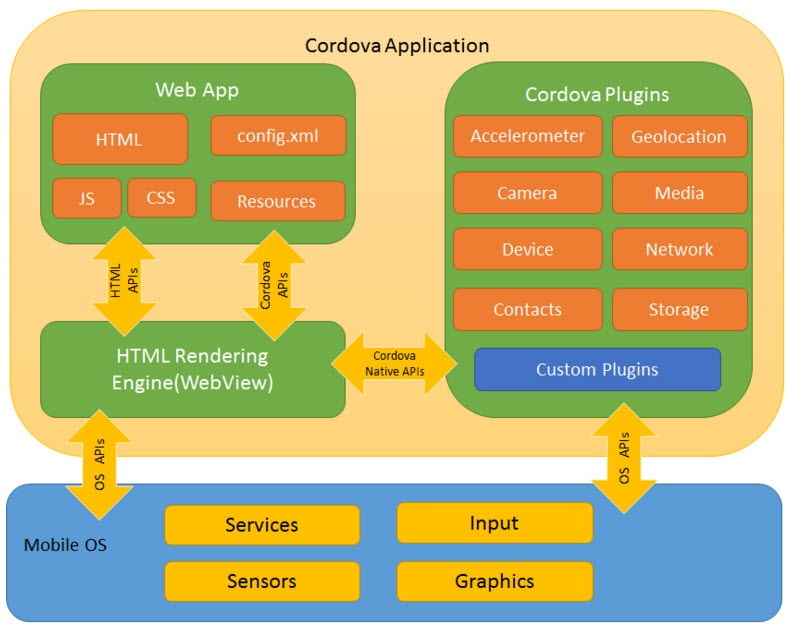
\includegraphics[width=0.8\columnwidth]{Figures/2/ionic2}
			\caption{Cordova Application}{ที่มา : http://blog.prscreative.com/what-is-ionic/}
			\label{Fig:ionic1}
		\end{figure}

		โดย Cordova มีหน้าที่ห่อหุ้มแอปพลิเคชันไว้ และทำหน้าที่ติดต่อกับ Hardware ของ Mobile เป็นหลักเพราะมี API ติดต่อกับ Hardware โดยตรง เช่น Camera, Contacts, Media, Network
		
		\subsubsection{ความแตกต่างระหว่าง PhoneGap/Cordova} 
		PhoneGap และ Cordova มีลักษณะคล้ายกัน เนื่องจากมันเกือบจะเหมือนกัน ต่างกันเพียงเรื่องของลิขสิทธิ์ และการนำไปใช้งาน

		\begin{enumerate}[label=\arabic*)]
		\item PhoneGap : ในยุคแรกถูกพัฒนาโดย Nitobi เปิดให้ใช้งานแบบ Open Source ซึ่งได้รับความนิยมในการนำมาใช้เป็นเทคโนโลยี Hybrid ซึ่งต่อมาถูกซื้อโดยบริษัท Adobe เพื่อนำมาเสริมทัพให้กับโปรแกรม Adobe Dreamweaver เพื่อให้สั่ง Build app จากโปรแกรม Dreamweaver ให้ลองรับหลาย Platform ได้ แต่มีค่าลิขสิทธิ์โปรแกรม
		\item Cordova : เกิดขึ้นจากการตกลงกันระหว่าง Adobe และ Nitobi ด้วยแนวคิดที่อยากให้ PhoneGap เป็น Open Source ต่อไป จึงได้มีการตกลงกันให้นำโค๊ดของ PhoneGap ไปตั้งเป็นชื่อใหม่ นั่นก็คือ Cordova เพื่อมอบให้ Apache Foundation ไปดูแลถูกนำไปใช้ในโครงการ Hybrid mobile application หลายโครงการ เช่น AppGyver, Ionic framework
		\end{enumerate}

		\subsubsection{ เริ่มต้นการใช้งาน}
		การเริ่มต้นใช้งาน Ionic Framework สามารถศึกษาการติดตั้งได้ที่ https://ionicframework.com/docs/v3/intro/installation/ ซี่งเริ่มต้นเราจะต้องทำการติดตั้ง Cordova CLI และ Ionic CLIผ่าน npm ก่อน
		\begin{figure}[H]
			{\setstretch{1.0}\begin{lstlisting}
$ npm install -g cordova 
# ติดตั้ง Cordova CLI
$ npm install -g ionic 
# ติดตั้ง Ionic CLI
$ ionic start ชื่อโปรเจค
# สร้างโปรเจคไอโอนิกมีลักษณะธีมเริ่มต้นเป็น Blank
$ cd ชื่อโปรเจค
# เข้าไปในโปรเจคที่เราสร้าง
$ ionic serve
# รันไอโอนิกแบบ localhost:8000
				\end{lstlisting}}
			\centering
			\caption{แสดงการติดตั้ง cli}
			\label{Fig:moment}
		\end{figure}


% Firebase

\subsection{Firebase}
	Firebase \cite{firebase} คือ บริการ Backend และ แพลตฟอร์ม ครบวงจรสำหรับนักพัฒนาแอปพลิเคชัน และโปรแกรมประยุกต์บนเว็บแพลตฟอร์มที่มีเครื่องมือและโครงสร้างพื้นฐานที่ได้รับการออกแบบมาเพื่อช่วยให้นักพัฒนาสามารถสร้างแอปพลิเคชันพลิเคที่มีคุณภาพสูง Firebase (ไฟร์เบส) ถูกสร้างขึ้นจากคุณสมบัติเสริมว่านักพัฒนาสามารถผสมและจับคู่เพื่อให้พอดีกับความต้องการของตน บริษัท ก่อตั้งขึ้นในปี 2011 โดยแอนดรูลีและเจมส์ เทมปลิน สินค้าเริ่มต้น Firebase) เป็นฐานข้อมูลเรียลไทม์ซึ่งมี API ที่ช่วยให้นักพัฒนาในการจัดเก็บและซิงค์ข้อมูล ดังรูป \ref{Fig:class1}
	
	Google Firebase 2.0 มีการพัฒนาจากบริการ Backend เก็บข้อมูลอย่างเดียว มาเป็น แพลตฟอร์มครบวงจรสำหรับนักพัฒนาแอปพลิเคชัน (รองรับ iOS, Android, Web) และรองรับบริการทุกอย่างที่นักพัฒนาแอปต้องการใช้งาน
	
	\begin{figure}[H]
		\centering
		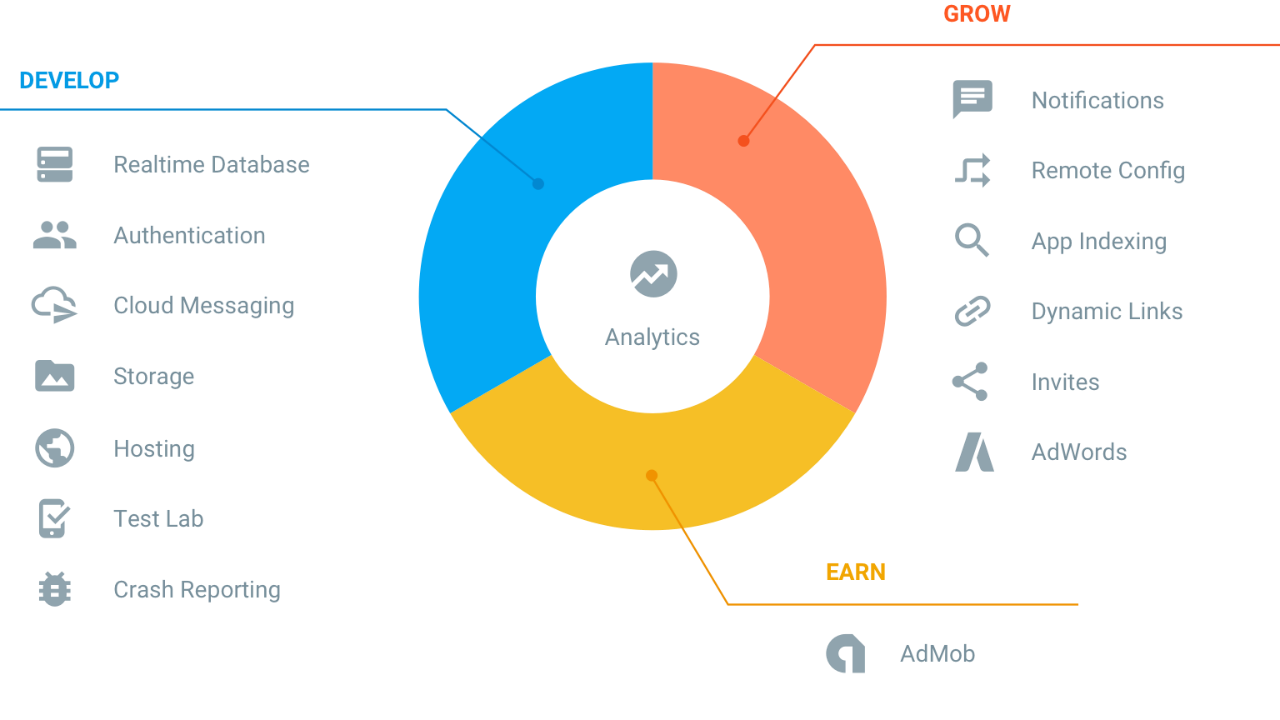
\includegraphics[width=\columnwidth]{Figures/2/firebase}
		\caption{Firebase 2.0}{ที่มา : www.mindphp/คู่มือ/73-คืออะไร/3921-what-is-firebase-backend.html}
		\label{Fig:class1}
	\end{figure}

\subsubsection{บริการหลักของไฟร์เบส} 

\begin{itemize}
	\item Realtime Database จัดเก็บและซิงค์ข้อมูลระหว่างผู้ใช้และอุปกรณ์ต่างๆแบบเรียลไทม์โดยใช้ฐานข้อมูล NoSQL ที่โฮสต์บนระบบคลาวด์ ซิงค์ข้อมูลที่อัปเดตระหว่างอุปกรณ์ที่เชื่อมต่อเป็นมิลลิวินาทีและข้อมูลจะยังคงมีอยู่ถ้าแอพพลิเคชันออฟไลน์
	\item Authentication จัดการบัญชีผู้ใช้ด้วย Firebase Auth ซึ่งใช้งานง่ายและปลอดภัยมีวิธีการหลายในการสร้างบัญชีผู้ใช้และตรวจสอบความถูกต้อง ได้แก่ อีเมล/รหัสผ่าน, ผู้ให้บริการบุคคลที่สามเช่น Google หรือ Facebook 
	\item Cloud Storage จัดเก็บภาพเสียงวิดีโอหรือเนื้อหาอื่น ๆ เช่น รูปภาพโปรไฟล์ผู้ใช้ หรือวีดีทัศน์ต่างๆ เป็นต้น ซึ่งมีความปลอดภัยในการอัปโหลดไฟล์และดาวน์โหลดสำหรับแอพพลิเคชัน
	\item Hosting ใช้ในการเผยแพร่เว็บไซต์  โดยเนื้อหาภายในเว็บเป็นเดชบอร์ด รายงานข้อต่างๆ ของผู้ใช้ ซึ่งต้องทำการเข้าสู่ระบบก่อน
	\item Crashlytics เป็นบริการล่าสุดที่กูเกิลได้เข้าควบรวมเข้ามาไว้ในบริการไฟร์เบส สามารถรายงานข้อขัดข้องได้อย่างมีประสิทธิภาพ เปิดใช้งานการวิเคราะห์แบบเรียลไทม์เพื่อช่วยให้เข้าใจสิ่งที่เกิดขึ้นในแอพพลิเคชัน เครื่องมือวิเคราะห์ข้อมูลจะให้ข้อมูลเชิงลึก
	\item Cloud Firestore เป็นบริการในส่วนของ Database ที่ใช้ระบบฐานของข้อมูลแบบ NoSQL ที่เป็นแบบ Document Database และเป็นการนำเอาข้อดีต่างๆของบริการด้านฐานข้อมูลของ Realtime Database มาปรับปรุงพัฒนาต่อและเพิ่มความสามารถขึ้นไปมากขึ้น ซึ่งผู้เขียนจะได้กล่าวถึงในบทถัดไป
\end{itemize}

\subsubsection{การพัฒนา Cloud Firestore} 
การพัฒนา Cloud Firestore แบ่งออกแบบ 5 ขั้นตอน ดังนี้

\begin{enumerate}[label=\arabic*)]
	\item การสร้าง Cloud Firestore เพื่อใช้งานในโครงการ ในขั้นตอนแรกทำการสร้าง Database เพื่อที่จะใช้งาน Cloud Firestore ก่อน โดยใช้บัญชี Gmail ต่อมาเข้าไปที่เว็บ https://firebase.google.com  ดังรูปภาพที่ \ref{Fig:f1}
	\begin{figure}[H]
		\centering
		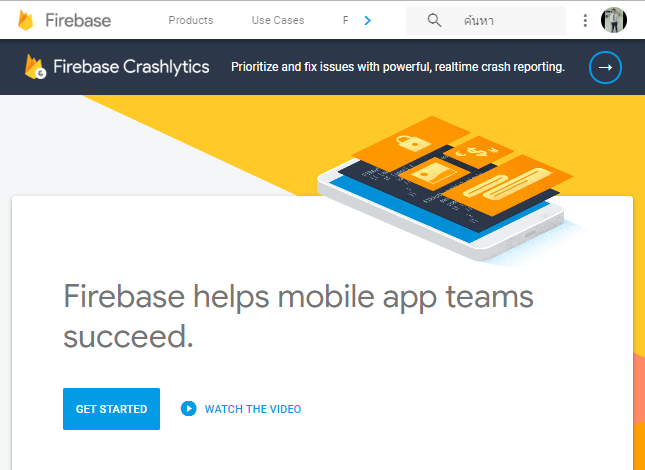
\includegraphics[width=0.7\columnwidth]{Figures/2/f1}
		\caption{เว็บ https://firebase.google.com}{ที่มา :https://medium.com/20scoops-cnx/เข้มข้นกับ-firebase-cloud-firestore-ระบบฐานข้อมูลที่เปิดตัวใหม่ล่าสุดจาก-firsbase-แบบจัดเต็ม-d001e43e2be7 }
		\label{Fig:f1}
	\end{figure}
	\item ติดตั้ง SDKs เพื่อใช้งาน Cloud Firestore
	โดย SDKs ที่ Firebase ได้เตรียมไว้ให้ สามารถดูรายละเอียดได้ที่ https://firebase.google.com/docs/firestore/quickstart
	\item ออกแบบโครงสร้างและการจัดการข้อมูล  
	\begin{itemize}
		\item ระบบฐานข้อมูลของ Cloud Firestore จะเป็น NoSQL แบบ Document ซึ่งจะแตกต่างจากระบบฐานข้อมูลแบบ SQL โดยจะไม่มีตาราง ไม่มีแถว แต่เก็บข้อมูล ภายใน Document จะเก็บแบบ Key-value โดยแต่ละ Document จะถูกเก็บไว้ใน Collection ซึ่งใน Document สามารถมี Subcollection ได้
		\item Collection เป็นการเรียกชื่อแทนของการเก็บหลายๆเอกสารไว้ด้วยกัน เช่น เก็บข้อมูลของ User จำนวนมากไว้ด้วยกัน จึงตั้งชื่อ Collection ว่า Users ซึ่งใน Collection เดียวกันผู้ใช้งานสามารถใส่ข้อมูลที่แตกต่างชนิดกันในแต่ละ Key แต่ละ Document ได้ โดยในแต่ละ Key และ Document จะมีอิสระในการใส่ข้อมูล แต่ควรใส่ข้อมูลในแต่ละ Key ของ Document เป็นประเภทเดียวกันเพราะจะทำให้การค้นหาและการจัดเรียงลำดับของข้อมูลนั้นง่ายขึ้น
		\item Subcollection สามารถสร้าง Subcollection ของ Subcollection ไปได้เรื่อยๆ โดย Cloud Firestore ว่าสามารถซ้อนกันไปได้ 100 ลำดับชั้น
	\end{itemize}
	\item การรับและสอบถามข้อมูล
	การรับและสอบถามข้อมูลจาก Cloud Firestore จะมี 2 วิธี โดยจะสามารถใช้ได้ทั้งการรับข้อมูลและการสอบถามข้อมูล
	\begin{itemize}
		\item การรับข้อมูลเพียงครั้งเดียวจะเป็นการรับข้อมูลเมื่อมีจุดประสงค์ที่จะไม่ต้องการรับรู้การเปลี่ยนแปลงของข้อมูล ซึ่ง ณ ขณะนั้นข้อมูลมีค่าเป็นอะไรก็จะได้ค่านั้นมา หากมีการเปลี่ยนแปลงข้อมูลในภายหลัง ผู้ใช้งานต้องเป็นผู้จัดการรับข้อมูลล่าสุดเอง โดยวิธีการรับข้อมูลเพียงครั้งเดียวจะใช้ Method Get()
		\item การรับข้อมูลแบบ Realtime update จะเป็นการรับข้อมูลเมื่อผู้ใช้งานมีจุดประสงค์ที่จะต้องการรับรู้การเปลี่ยนแปลงของข้อมูล ซึ่ง ณ ขณะที่ข้อมูลเกิดการเปลี่ยนแปลงจะมีการรับข้อมูลที่เกิดการเปลี่ยนแปลงโดยอัตโนมัติ โดยในครั้งแรกที่มีการรับข้อมูลจะสร้าง Initialize Instance และทุกครั้งที่ข้อมูลมีการเปลี่ยนแปลงก็จะส่ง Callback ให้กับ Iistener โดยผ่าน Method onSnapshot()
	\end{itemize}
	\item การป้องกันและความปลอดภัยของข้อมูลข้อมูลใน Cloud Firestore ได้มีการออกแบบให้สามารถกำหนดกฏของความปลอดภัยต่างๆได้ โดยผ่าน Firebase Console  ซึ่งหากใช้ Cloud Firestore ผู้ใช้งานสามารถมาทำเรื่องการป้องกันและรักษาความปลอดภัยของข้อมูลเพียงที่เดียวก็สามารถใช้ได้ทั้งหมดไม่ว่าจะเป็น Web และ Mobile ส่วนฝั่ง Server ก็สามารถใช้ IAM ใน Google Cloud Platform มาจัดการความปลอดภัยสำหรับ Cloud Firestore ได้
\end{enumerate}


% Dialogflow

\subsection{Dialogflow}
Dialogflow คือ platform สำหรับสร้าง chatbot ของ Google ที่ใช้ machine learning ด้าน Natural Language Processing (NLP) มาช่วยในทำความเข้าใจถึงความต้องการ (intent) และสิ่งที่ต้องการ (entity) ในประโยคสนทนาของผู้ใช้งาน และตอบคำถามตามความต้องการของผู้ใช้งาน ตามกฎ หรือ flow ที่ผู้พัฒนาวางเอาไว้ ซึ่ง Dialogflow จะช่วยเพิ่มความยืดหยุ่นของประโยคที่ chatbot รับมา ว่าไม่จำเป็นต้องตรงตามเงื่อนไข แบบ rule based ก็สามารถเข้าใจถึงความต้องการของผู้ใช้งานได้

 \begin{figure}[H]
	\centering
	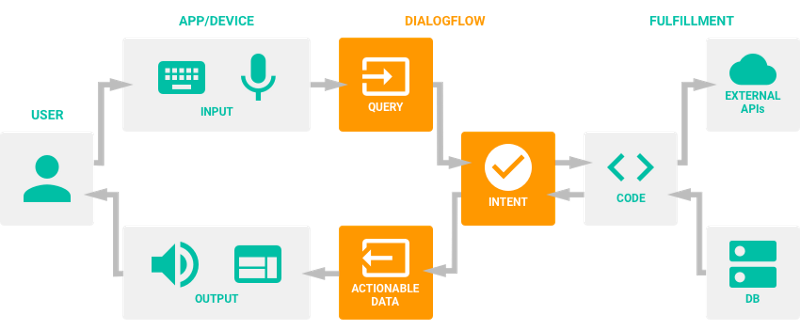
\includegraphics[width=0.9\columnwidth]{Figures/2/chatbot}
	\caption{รูปแบบการส่งข้อมูลผู้ใช้ไปยังแชทบอท}{ที่มา : https://dialogflow.com/docs/agents}
	\label{Fig:dialogflow}
\end{figure}

\subsubsection{เริ่มต้นใช้งาน Dialogflow} 

\begin{enumerate}[label=\arabic*)]
\item ลงทะเบียน/ล๊อกอินเข้า Dialogflow \\
ในการสร้าง Agent เราต้องลงทะเบียนเข้าใช้งานก่อนนะ โดยไปยังหน้าเว็บของ Dialogflow และกดที่ Go Console จากนั้นก็เข้าสู่ขั้นตอนการ Login หรือลงทะเบียน

	\begin{figure}[H]
		\centering
		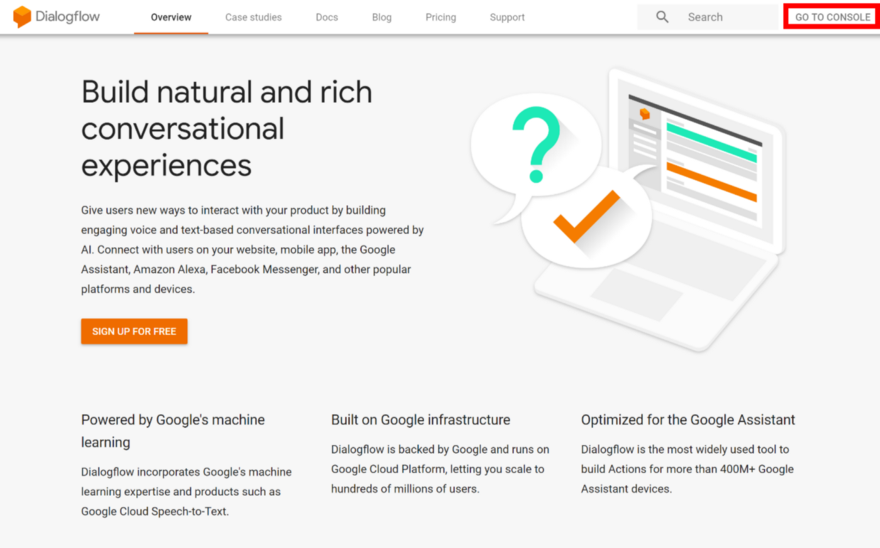
\includegraphics[width=0.9\columnwidth]{Figures/2/dialogflow_1}
		\caption{หน้าหลักของ Dialogflow}
		\label{Fig:dialogflow1}
	\end{figure}

\item สร้าง Agent \\
หลังจาก Login สำเร็จเราก็จะเจอกับ Workplace ในการทำแชทบอทละ ให้ไปที่เมนูด้านซ้าย และเลือก Create Agent ก็จะพบกับหน้าจอสำหรับตั้งค่าแชทบอทของเรา โดยต้องสามารถตั้งชื่อ ภาษา และ Timezone ที่ต้องการ

	\begin{figure}[H]
		\centering
		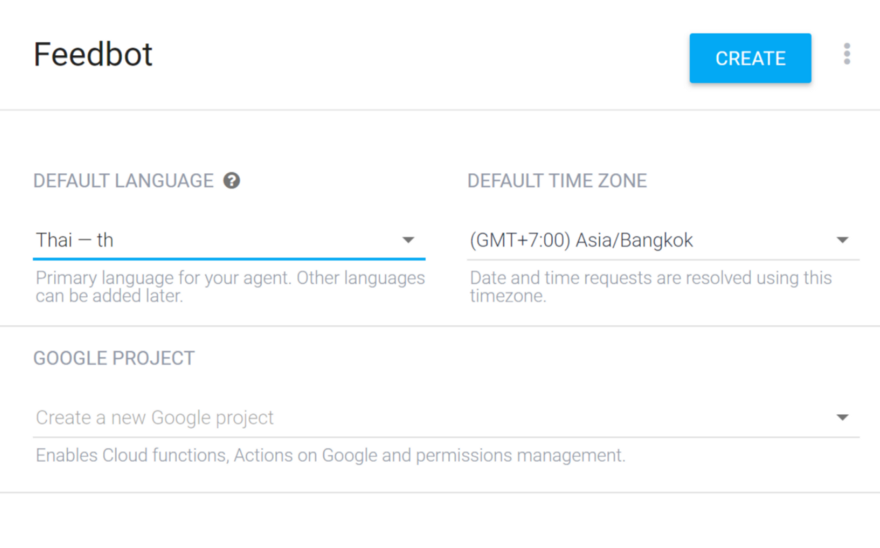
\includegraphics[width=0.9\columnwidth]{Figures/2/dialogflow_2}
		\caption{หน้า Create Agent}
		\label{Fig:dialogflow2}
	\end{figure}

\item สอนบอทให้พูดทักทาย \\
เมื่อสร้างเสร็จแล้วเราจะพบกับ Default Intents มา 2 ตัวก็คือ Default Welcome Intent และ Default Fallback Intent มาให้ ตอนนี้ยังไม่ต้องสนใจมันนะ เพราะเราจะลองสร้าง Intent ใหม่เลยโดยตั้งชื่อว่า Greeting 
ในการสร้างให้กดที่ปุ่ม Create Intent และตั้งชื่อ Intent นี้ว่า Greeting โดยเราตั้งใจจะให้ Intent นี้ โต้ตอบกับผู้ใช้งาน เวลาที่ผู้ใช้ต้องการที่จะทักทายกับแชทบอท ที่เราสร้างขึ้นมา
จากนั้นไปที่ Training phrases หรือแนวประโยคที่เราจะให้แชทบอทเข้าใจว่า ถ้าพูดด้วยประโยคประมาณนี้ แสดงว่าผู้ใช้งานตั้งใจจะสื่อถึง Intent นี้ ถ้าดูจากตัวอย่างจะพบว่ามีการระบุ phrases ไว้ว่า สวัสดี, สวัสดีจ้ะ, สวัสดีจ้า

	\begin{figure}[H]
		\centering
		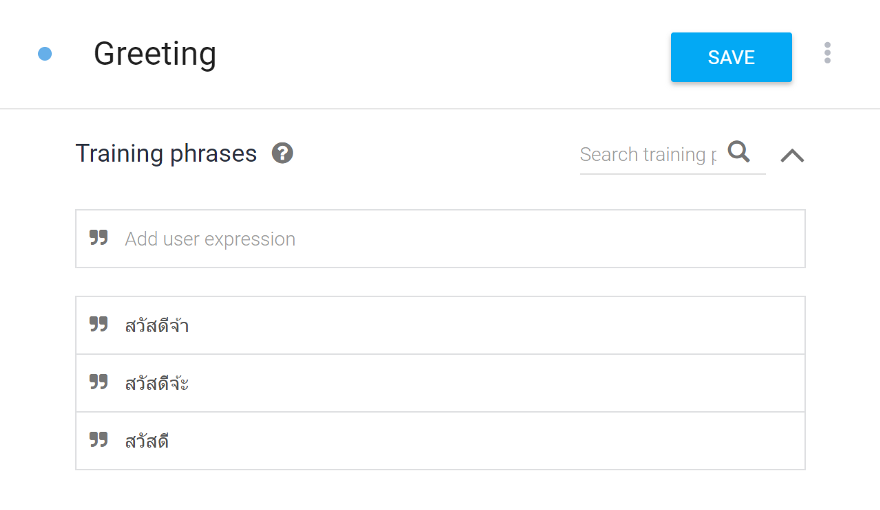
\includegraphics[width=0.9\columnwidth]{Figures/2/dialogflow_3}
		\caption{หน้า Intent ส่วน Training phrases}
		\label{Fig:dialogflow3}
	\end{figure}
	
จากนั้นเราจะลองไปตั้งค่า Responses หรือประโยคที่เราต้องการให้แชทบอทตอบกลับ ในกรณีนี้ที่บอทสามารถจับได้ว่าผู้ใช้งานตั้งใจจะสื่อถึง Intent นี้ สำหรับตัวอย่างจะพบว่า ถ้าผู้ใช้พิมพ์ สวัสดี, สวัสดีจ้ะ, สวัสดีจ้า ตาม Training phrases เราจะให้แชทบอทของเราตอบกลับว่า สวัสดีครับ เป็นยังไงบ้างครับ สบายดีไหม หรือ สวัสดีครับ สบายดีไหมครับ โดยจะสุ่มขึ้นมาว่าจะตอบอันไหน
	
	\begin{figure}[H]
		\centering
		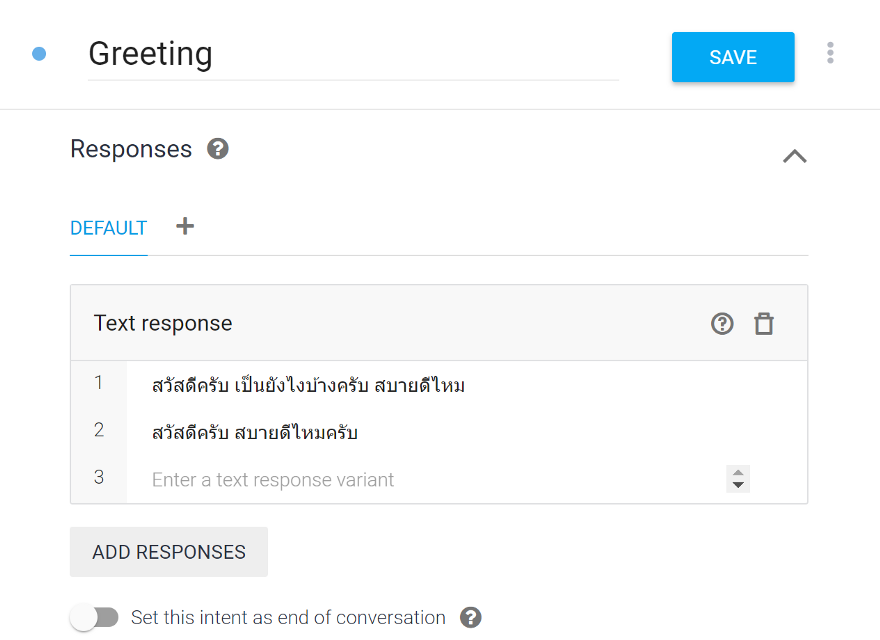
\includegraphics[width=0.9\columnwidth]{Figures/2/dialogflow_4}
		\caption{หน้า Intent ส่วน Responses}
		\label{Fig:dialogflow4}
	\end{figure}


ตรงส่วนของ Responses เราสามารถเพิ่มข้อความ หรือเพิ่ม balloon message ให้ต่อกันหลายๆอันได้ โดยกดที่ปุ่ม Add Responses และถ้าต้องการตั้งค่าว่า intent นี้เป็น intent สุดท้ายในการสนทนากัน ก็สามารถเปิด Checkbox Set this intent as end of conversation ซึ่งเดียวเราค่อนมาคุยกันแบบละเอียดอีกครั้ง ตอนที่ต้องทำ Contexts กันอีกครั้ง

\item ทดสอบคุยกับบอท \\
หลังจากเราลองทำ Greeting Intent เสร็จ ก็ถึงเวลาที่เราจะลองทดสอบการใช้งานกัน ซึ่งเราสามารถทดสอบได้ผ่านกล่องสนทนาที่อยู่ทางด้านขวา โดยลองพิมพ์คำว่า สวัสดี ลงไป ก็จะพบว่าแชทบอทจะตอบเรากลับมาว่า สวัสดีครับ เป็นยังไงบ้างครับ สบายดีไหม ตามที่เราตั้งค่าไว้ใน Responses นั้นเอง

	\begin{figure}[H]
		\centering
		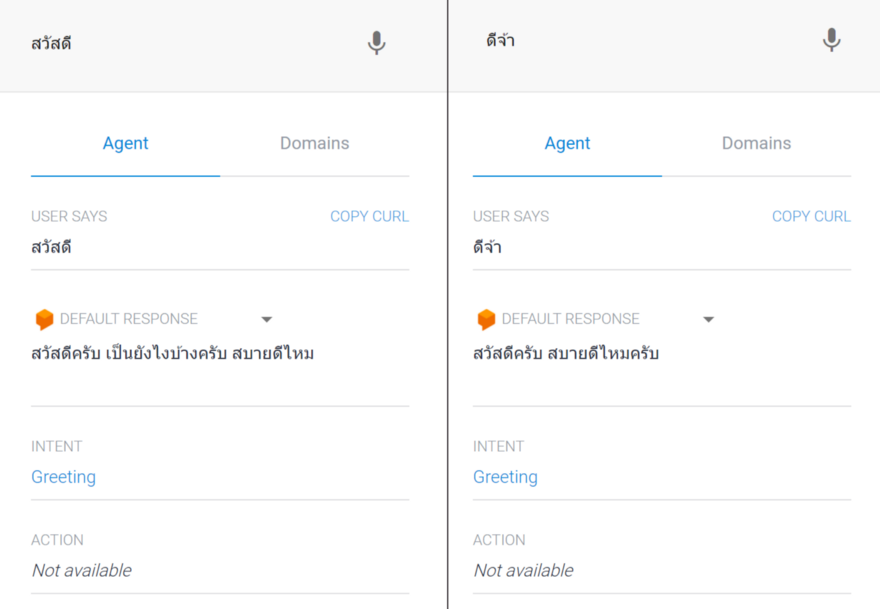
\includegraphics[width=0.9\columnwidth]{Figures/2/dialogflow_5}
		\caption{ทดสอบคุยกับบอท}
		\label{Fig:dialogflow5}
	\end{figure}

ถ้าดูจากภาพ \ref{Fig:dialogflow5} จะพบว่า ถ้าเราพิมพ์คำบางคำที่ไม่ได้มีอยู่ใน Training phrases อย่างคำว่า ดีจ้า ตัว Dialogflow ก็ฉลาดพอที่จะจับได้ว่านี่คือคำที่อยู่ในกลุ่มเดียวกับ สวัสดี ซึ่งเป็นคำทักทาย ที่เรากำหนดว่ามันคือ Intent Greeting นั้นเอง

แต่ในขณะเดียวกัน คำบางคำ หรือประโยคบางประโยคตัวแชทบอทของเราก็อาจจะยังไม่เข้าใจ ว่าสิ่งที่ผู้ใช้งานต้องการจะสื่อสารออกมา มันคือ Intent อะไร ซึ่งเวลาสร้าง Agent Dialogflow ก็จะสร้าง Default Fallback Intent ขึ้นมาให้ พร้อมกับ Responses บางส่วน ในกรณีที่แชทบอทไม่สามารถหา Intent ที่เหมาะสมได้ ก็จะมาตกที่เคสนี้ทั้งหมดตามภาพนั้นเอง

	\begin{figure}[H]
		\centering
		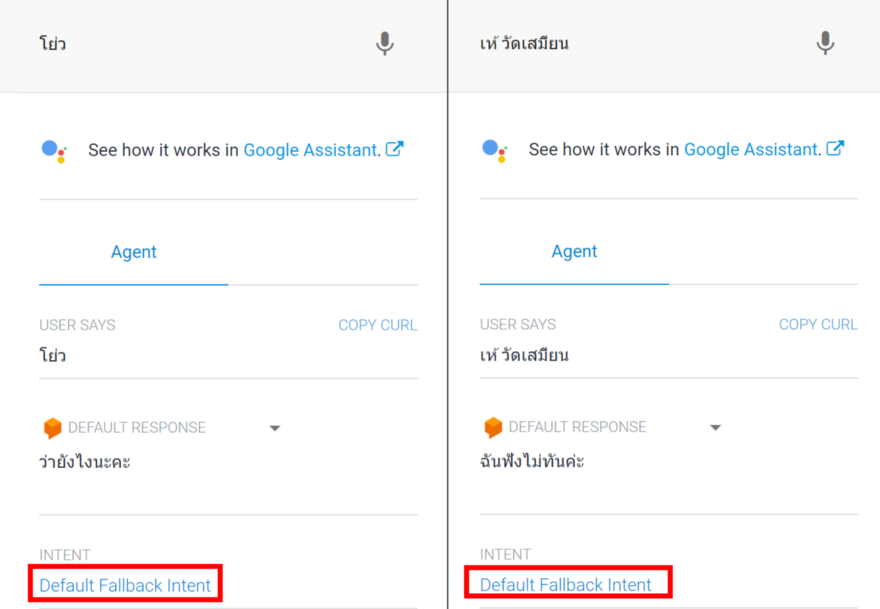
\includegraphics[width=0.9\columnwidth]{Figures/2/dialogflow_6}
		\caption{ทดสอบคุยกับบอท}
		\label{Fig:dialogflow6}
	\end{figure}

\end{enumerate}



\subsection{Libraries moment.js}
moment.js คือ javascript library สำหรับใช้สำหรับจัดการ Date และ Time ที่จะช่วยอำนวยความสะดวกในเรื่องการจัด Format Date ให้ตรงกับที่เราต้องการ
มี Feature ที่หลากหลายครอบคลุมทั้งใช้งาน Format ทั้ง Date , Time , Timezone , Standard Time , Local Time เป็นต้น ซึ่งการนำ library moment.JavaScript 
มาใช้งานสามารถติดตั้งได้ดังนี้

\subsubsection{คำสั่งในการติดตั้ง}
	\begin{figure}[H]
		{\setstretch{1.0}\begin{lstlisting}
/*  install dependency */
npm install moment --save   # npm
yarn add moment             # Yarn
Install-Package Moment.js   # NuGet
spm install moment --save   # spm
meteor add momentjs:moment  # meteor
bower install moment --save # bower (deprecated)
		\end{lstlisting}}
	\centering
		\caption{คำสั่งในการติดตั้ง moment.js}
		\label{Fig:momentjs}
	\end{figure}

\subsubsection{รูปแบบการใช้งาน moment.js}
	\begin{figure}[H]
		{\setstretch{1.0}\begin{lstlisting}
const moment = require('moment');

const SLASH_DMY = 'DD/MM/YYYY';
const SLASH_DMYHMS = 'DD/MM/YYYY HH:mm:ss';
const SLASH_YMD = 'YYYY/MM/DD';
const SLASH_YMDHMS = 'YYYY/MM/DD HH:mm:ss';
const DASH_DMY = 'DD-MM-YYYY';
const DASH_DMYHMS = 'DD-MM-YYYY HH:mm:ss';
const DASH_YMD = 'YYYY-MM-DD';
const DASH_YMDHMS = 'YYYY-MM-DD HH:mm:ss';
			
console.log('sysdate ::==',moment());
			
console.log('sysdate ::==',moment().format(SLASH_DMY));
console.log('sysdate ::==',moment().format(SLASH_DMYHMS));
			
console.log('sysdate ::==',moment().format(SLASH_YMD));
console.log('sysdate ::==',moment().format(SLASH_YMDHMS));
			
console.log('sysdate ::==',moment().format(DASH_DMY));
console.log('sysdate ::==',moment().format(DASH_DMYHMS));
			
console.log('sysdate ::==',moment().format(DASH_YMD));
console.log('sysdate ::==',moment().format(DASH_YMDHMS));
/*
sysdate ::== moment("2018-07-03T21:08:38.248")
sysdate ::== 03/07/2018
sysdate ::== 03/07/2018 21:08:38
sysdate ::== 2018/07/03
sysdate ::== 2018/07/03 21:08:38
sysdate ::== 03-07-2018
sysdate ::== 03-07-2018 21:08:38
sysdate ::== 2018-07-03
sysdate ::== 2018-07-03 21:08:38
*/
		\end{lstlisting}}
	\centering
		\caption{รูปแบบการใช้งาน moment.js}
		\label{Fig:howtomomentjs}
	\end{figure}

ทั้งหมดที่ยังไม่ใช้ทั้งหมดที่ Moment JS ทำได้ยังมีความสามารถอีกหลายอย่างที่ยังไม่ได้กล่าวถึงที่ Moment ทำได้เข้าไปดูได้ที่ https://momentjs.com/docs/

\subsection{Google Maps API}

Google Maps คือ บริการแผนที่ของ Google ซึ่งให้บริการ Services ที่เกี่ยวข้องกับแผนที่ทั้งหมด โดยในปัจจุบันแผนที่ของ Google
นั้นมีอยู่หลากหลายประเภท อาทิเช่นที่เราใช้บริการแผนที่บนเว็บไซต์ หรือ App บน Smartphone โดย Services เหล่านี้เราสามารถ
เรียกใช้ได้ฟรีในกรณีที่ผ่าน Application ทั่วไป แต่ถ้าในกรณีที่เราจะมีการเรียกใช้งานในเว็บไซต์หรือแอปพลิเคชันที่พัฒนาขึ้นเอง Google Maps 
ก็จะมี API ให้ใช้งานได้เช่นเดียวกัน แต่ Services ของ Google นั้นมีข้อจำกัดในการใช้งาน ถ้าต้องการใช้ในปริมาณที่สูงขึ้นก็จะต้องซื้อ Package 
ที่ทาง Google Maps มีมาให้ โดยปกติจะมีการจำกัดจำนวนที่ Request เข้ามาเรียกใช้งาน สำหรับเรียกใช้แผนที่และชุด service ต่าง ๆ ของ Google 
เพื่อพัฒนา Application ได้เหมือนกับ Google มีบริการ features ให้เรียกใช้ดังต่อไปนี้

	\begin{itemize}
		\item การปรับแต่งแผนที่ (Styled Map)
		\item ชุดควบคุมแผนที่ (Map Control)
		\item ชุดเครื่องมือวาดภาพบนแผนที่ (Drawing)
		\item การนำทางจากจุดหนึ่งไปยังอีกจุดหนึ่ง (Directions Service)
		\item การคำนวณความสูงของจุดพิกัด (Elevation Service)
		\item การแปลงที่อยู่เป็นพิกัด Lattitude เเละ Longtitude (GeoCoding Service)
		\item การดึงข้อมูล POI (Point of Interest)
		\item Street View
	\end{itemize}

	ประโยชน์ของการใช้งาน Google Maps

	\begin{itemize}
		\item สามารถค้นหาสถานที่ต่าง ๆ ได้อย่างสะดวกรวดเร็ว
		\item สามารถค้นหาชื่อถนนและสี่แยกได้
		\item สามารถค้นหาร้านอาหารในพื้นที่ที่ต้องการได้
		\item สามารถที่จะประชาสัมพันธ์สถานประกอบการทางธุรกิจ
		\item สามารถย่อหรือขยายแผนที่ทั่วโลกให้เล็กลงได้
		\item สามารถวางแผนเส้นทางการเดินทางไปยังพื้นที่ต่าง ๆ ได้
		\item สามารถใช้งานด้านระบาดวิทยาในการค้นหาแหล่งแพร่เชื้อ
		\item สามารถทำแผนที่หรือเส้นทางไปบ้านของตนเองได้
		\item สามารถแสดงตำแหน่งของตนเองได้
		\item สามารถดูและมองเห็นแผนที่ต่าง ๆ ทั่วโลกได้อย่างรวดเร็ว
	\end{itemize}

	การนำ Google Maps API มาใช้งาน

	สิ่งที่ต้องทำเพื่อเรียก Google Maps API มาใช้งานดังนี้
	\begin{enumerate}[label=\arabic*)]
		\item ทำการสมัครขอ API KEY โดยสามารถเข้าไปสมัครได้ที่ https://console.developers.google.com
		\item เพิ่มคำสั่งในบรรทัดที่ 2 ไว้ในไฟล์ index.html
		
		\begin{figure}[H]
			{\setstretch{1.0}\begin{lstlisting}
<head>
<script src="https://maps.googleapis.com/maps/api/js?key={API_KEY}" async defer></script>
</head>
		\end{lstlisting}}
	\centering
		\caption{เรียกใช้ API KEY}
		\label{Fig:googlemapapi}
	\end{figure}

	\item ขั้นตอนการเรียกใช้งานสำหรับแสดง Google Maps
	
	\begin{figure}[H]
		{\setstretch{1.0}\begin{lstlisting}
<-- IN HTML -->

<div #map id="map"></div> // เรียกใช้ map เพื่อแสดง

<-- IN TYPESCRIPT -->

map:any; //กำหนดตัวแปร map

ionViewDidLoad() {
  this.initMap();
} // เรียกใช้งานเมื่อหน้านี้ถูกเรียก

initMap() {
  this.map = new google.maps.Map(this.mapElement.nativeElement, {
    zoom: 7,
    center: {lat: 41.85, lng: -87.65}
  });
  this.directionsDisplay.setMap(this.map);
} // ฟังก์ชันสำหรับกำหนด map

<-- IN SCSS -->
	#map {
		height: 100%;
	} // ขนาดของ map
					
				\end{lstlisting}}
			\centering
				\caption{เรียกใช้งาน google maps ใน ionic framework}
				\label{Fig:googlemapionic}
			\end{figure}
			\item เรียกใช้งานด้วยคำสั่ง Google Maps เพื่อใช้งานตามต้องการ
		\end{enumerate}
		
	  

\section{เอกสารและงานวิจัยที่เกี่ยวข้อง}
\subsection{แอปพลิเคชันเครือข่ายสังคมออนไลน์เพื่อผู้สูงอายุ (OLDSTER) }
แอปพลิเคชันเครือข่ายสังคมออนไลน์เพื่อผู้สูงอายุ (OLDSTER) \cite{oldsterref} เป็นแอปพลิเคชันที่ถูกออกแบบมาเป็นเครือข่ายสังคมของผู้สูงอายุ โดยแอปพลิเคชันนี้ถูกออกแบบเพื่อผู้สูงอายุเป็นหลัก จึงง่ายต่อการใช้งาน มีรูปแบบที่ไม่ยุ่งยาก ไม่ซับซ้อน ตัวหนังสือเป็นแบบที่ง่ายต่อการอ่าน และขนาดไม่เล็กเกินไป 
มีฟังก์ชันการทำงาน 9 ฟังก์ชันดังนี้ ข้อมูลส่วนตัว กระดานข่าว พูดคุยระหว่างผู้ใช้งาน การแจ้งเตือน วิธีใช้งาน ข่าวสารในหมวดต่าง ๆ เป็นต้น โดยความแตกต่างระหว่างแอปพลิเคชัน OLDSTER กับ สูงวัยมายเฟรนด์ อยู่ตรงที่แอปพลิเคชันสูงวัยมายเฟรนด์
จะมีการให้ความรู้ในเรื่องโรคที่ผู้สูงอายุมักพบเจอในรูปแบบของแชทบอท และยังมีการแชทแบบกลุ่ม การค้นหาตำแหน่งของคนในครอบครัว รวมทั้งมีการแจ้งเตือนการทานยาอีกด้วย
\begin{figure}[H]
\centering
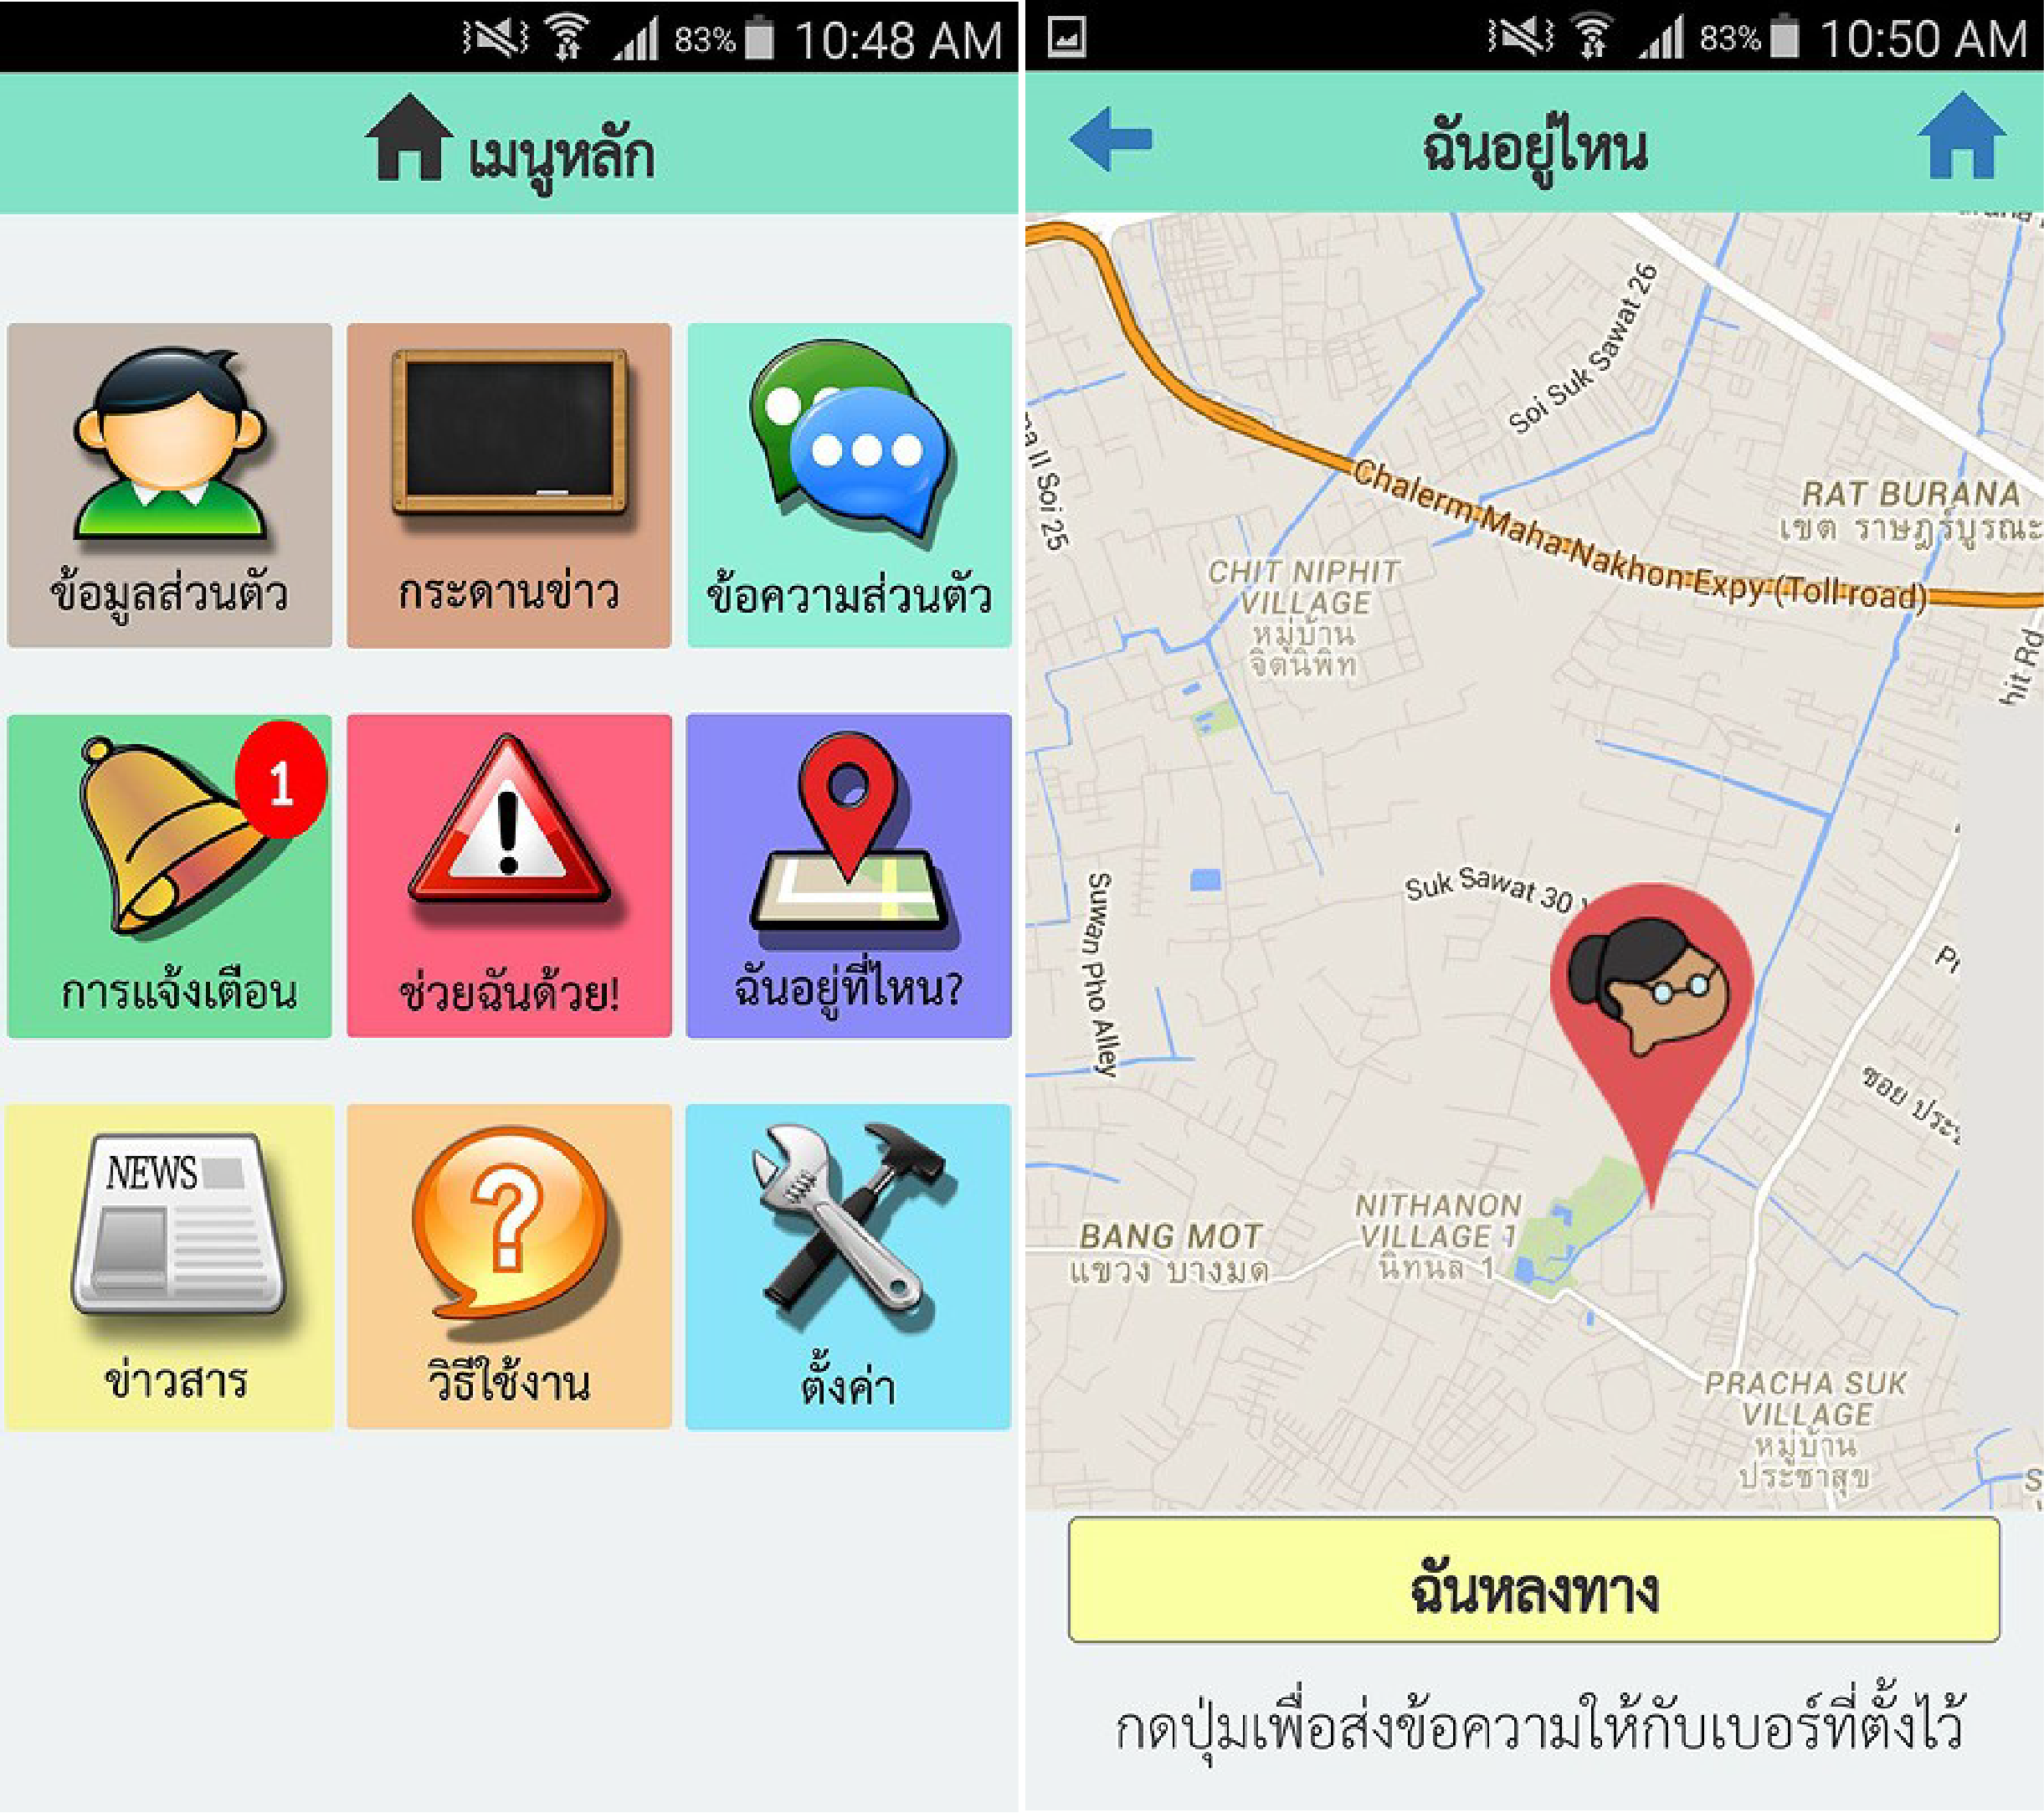
\includegraphics[width=0.8\textwidth]{Figures/2/oldsterfull}
\caption{แอปพลิเคชัน OLDSTER}
\label{Fig:ref1}
\end{figure}
	
\subsection{จับใจบอท}
จับใจบอท \cite{eStudentloan} เป็นแชทบอทที่สามารถพูดคุยได้ใน Messanger ของ Facebook เป้าหมายหลักคือเป็นแชทบอทที่ช่วยประเมินอาการซึมเศร้าของผู้ใช้งานได้ หากพบว่าตัวเองมีอาการซึมเศร้าก็จะช่วยในการตัดสินใจในการพบแพทย์ได้เร็วขึ้น 

\newpage
\begin{figure}[H]
	\centering
	
\includegraphics[width=0.8\textwidth]{Figures/2/ref2}
	\caption{แชทบอทของ จับใจบอท}{ที่มา : https://techsauce.co/tech-and-biz/jubjai-depression-detection-chatbot/}
	\label{Fig:ref2}
\end{figure}

ความแตกต่างระหว่าง จับใจบอท กับแอปพลิเคชันสูงวัยมายเฟรนด์ คือจับใจบอทเป็นการประเมินอาการซึมเศร้าเพียงอย่างเดียว ส่วนแอปพลิเคชันสูงวัยมายเฟรนด์จะแนะนำสาเหตุ และวิธีดูแลรักษาในเบื้องต้นให้แก่ผู้ใช้งาน



\chapter{การวิเคราะห์และออกแบบระบบ}

การวิเคราะห์และออกแบบระบบก่อนดำเนินการจริงเป็นอีกหนึ่งขั้นตอนที่มีความสำคัญมาก เพราะการวิเคราะห์และออกแบบระบบนั้นเป็นการกระทำที่ทำให้ผู้พัฒนาเห็นรายละเอียดส่วนย่อยของงานทั้งหมด เพิ่มประสิทธิภาพในการวางแผน การทำงาน และยังช่วยลดปัญหาที่อาจจะเกิดขึ้นในระหว่างพัฒนา เพื่อให้ระบบมีความสมบูรณ์มากยิ่งขึ้น เนื่องจากการวิเคราะห์และออกแบบระบบนั้นจะช่วยให้ให้บริการ จัดการทรัพยากรได้อย่างคุ้มค่าและตรงตามความต้องการของระบบ

การวิเคราะห์และออกแบบระบบ XX ในบทนี้จะแบ่งออกเป็น X ข้นตอนเพื่อให้เห็นการดำเนินงานอย่างมีระบบ ในหัวข้อแรกจะนำเสนอภาพรวมของระบบ ก่อนจะนำเสนอเอกสารแสดงความต้องการของระบบซึ่งจะทำให้เห็นที่มาของเพจต่าง ๆ ในขั้นตอนของการออกแบบในหัวข้อที่สาม ส่วนหัวข้อที่เหลือจะแสดงแผนภาพการการทำงานของระบบโดยใช้ UML diagram ซึ่งประกอบไปด้วย Use Case, Class และ Sequence Diagram เพื่อแสดงรายละเอียดของระบบก่อนนำไปเขียนคำสั่งด้วยภาษาโปรแกรมในบทต่อไป

\begin{enumerate}[label=3.\arabic*]
	\item โครงสร้างภาพรวมของระบบ (System Architecture) เป็นการออกแบบภาพรวมและเทคโนโลยีของระบบ
	\item System Requirements คือ ความต้องการหรือสิ่งที่ระบบควรจะทำ หรือหน้าที่หลักของ
	ระบบที่จะต้องทำ
	\item User Interface Design เป็นการออกแบบส่วนต่อประสานกับผู้ใช้
	\item Use Case Diagram เป็นแผนภาพที่ใช้แสดงให้ทราบว่าระบบทำงานหรือมีหน้าที่ใดบ้าง
	\item Class Diagram เป็นแผนภาพที่ใช้แสดง Class และความสัมพันธ์ระหว่าง Class
	\item Sequence Diagram เป็นแผนภาพที่ใช้แสดงให้เห็นถึงการตอบโต้ข้อมูลระหว่างคลาส เรียงตามลำดับของเวลาที่เกิดเหตุการณ์จากน้อยไปมาก
\end{enumerate}	

\section{โครงสร้างภาพรวมของระบบ}
    ความหมายของ System Architecture \cite{architecture} หมายถึง กรอบโครงสร้างของระบบที่อธิบายความสัมพันธ์ขององค์ประกอบต่าง ๆ ไปจนถึงขั้นการเชื่อมต่อกันของระบบย่อยต่าง ๆ โดยจัดกลุ่มองค์ประกอบไว้ในหลาย ๆ ลักษณะเพื่อให้ผู้เกี่ยวข้อง (Stakeholder) จากพื้นฐานสาขาอาชีพที่แตกต่าง กันสามารถทำความเข้าใจได้ง่าย เช่น การจัดแบ่งองค์ประกอบตามลักษณะการทำงานของระบบ (functional components) เป็นต้น
    
    การออกแบบ System architecture แสดงภาพรวมและเทคโนโลยีของระบบกองทุนเงินให้กู้ยืมเพื่อการศึกษา คณะวิทยาศาสตร์ มหาวิทยาลัยอุบลราชธานี มีรายละเอียดดังรูปที่ \ref{Fig:architecture}
   	\begin{figure}[H]
   		\centering
   		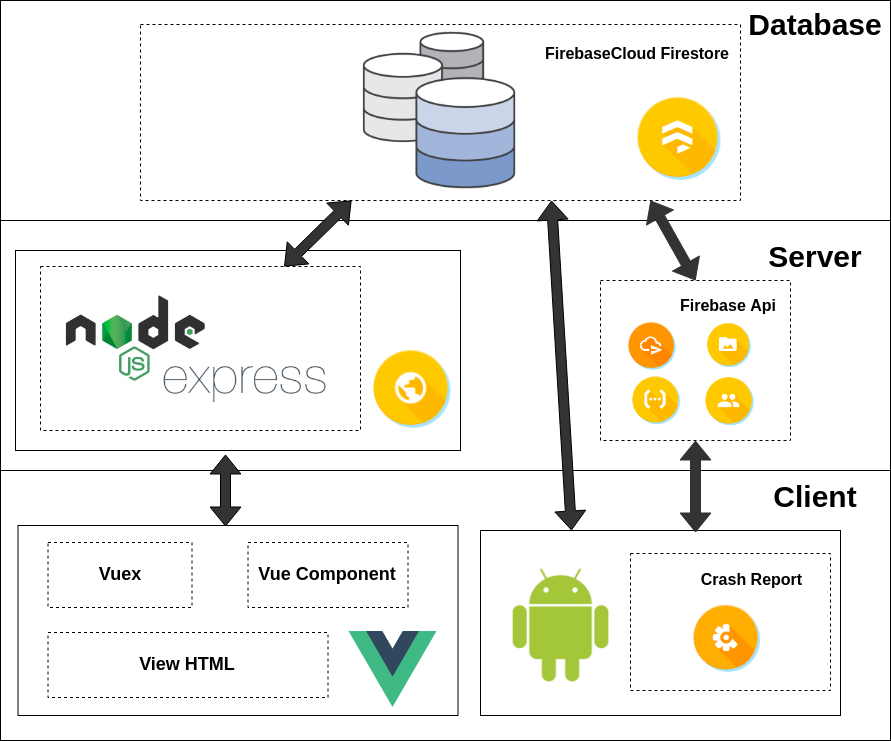
\includegraphics[width=\textwidth]{Figures/3/architecture/architecture}
   		\caption{System architecture ระบบ XX}
   		\label{Fig:architecture}
   	\end{figure}
   
   จากรูปที่ \ref{Fig:architecture} สามารถอธิบายโครงสร้างและเทคโนโลยีของระบบโดยแบ่งเป็น 3 ส่วนหลัก ดังนี้
   \begin{enumerate}
   	\item Database
   	 ระบบใช้บริการฐานข้อมูลแบบ NoSQL ของไฟร์เบสชื่อ Cloud Firestore
	  \item Server
	   กระบวนการทำงานในส่วนของเซิฟเวอร์ (server) แบ่งเป็น 2 ส่วนได้แก่
	   \begin{itemize}
	   	\item ไฟร์เบส Hosting เป็นบริการสำหรับสร้างโฮสต์ (Host) สำหรับเก็บซอร์สโค้ด (source code) และทำการเผยแพร่สำหรับการพัฒนาเว็บไซต์ ซึ่งในที่นี้ใช้ Node.js และ Express ในการพัฒนา
	   	\item ชุดบริการไฟร์เบส Api ใช้สำหรับการทำงานกับบริการต่าง ๆ ของไฟร์เบสบนแฟลตฟอร์มที่แตกต่างกัน เช่น Authentication ใช้สำหรับการจัดการข้อมูลผู้ใช้หรือไฟร์เบส Storage ที่ใช้สำหรับจัดเก็บไฟล์เอกสารและรูปภาพต่าง ๆ เป็นต้น
	   \end{itemize}
	   \item Client
	    แอปพลิเคชันของระบบกองทุนเงินให้กู้ยืมเพื่อการศึกษา คณะวิทยาศาสตร์ มหาวิทยาลัยอุบลราชธานี แบ่งเป็น 2 ส่วนตามการทำงานบนแฟลตฟอร์ม ดังนี้
	    \begin{itemize}
	    	\item เว็บแอปพลิเคชันวัตถุประสงค์ในใช้งานเพื่อรองรับการทำงานของผู้ใช้งานบนบราวเซอร์โดยพัฒนาด้วย Vue.js
	    	\item โมบายแอปพลิเคชันทำงานบนอุปกรณ์พกพา มีการใช้บริการ Crashlytics ของไฟร์เบสในการติดตามข้อผิดพลาดต่าง ๆ ที่เกิดขึ้น
	    \end{itemize}
   \end{enumerate}

\section{System Requirements}
\subsection{Functional Requirements}
	ระบบกองทุนเงินให้กู้ยืมเพื่อการศึกษา คณะวิทยาศาสตร์ มหาวิทยาลัยอุบลราชธานี แบ่งความสามารถของระบบตามประเภทของผู้ใช้งานดังนี้
	\begin{enumerate}
		\item เจ้าหน้าที่
			\begin{itemize}[label={--}]
				\item สามารถทำการเข้าสู่ระบบได้
				\item สามารถสร้างประกาศหรือประชาสัมพันธ์บนเว็บแอปพลิเคชันได้
				\item สามารถกำหนดวันที่และช่วงเวลาในการส่งเอกสารการกู้ยืมของกองทุนเงินให้กู้ยืมเพื่อการศึกษาได้
				\item สามารถตรวจสอบยืนยันความถูกต้องเอกสารกองทุนเงินให้กู้ยืมเพื่อการศึกษาจากนักศึกษาผ่านเว็บแอปพลิเคชันได้
				\item สามารถทำการอัพโหลดฐานข้อมูลนักศึกษากองทุนเงินให้กู้ยืมเพื่อการศึกษาได้
				\item สามารถส่งข้อความเพื่อติดต่อนักศึกษาในระบบได้
				\item สามารถทำการอัพโหลดเอกสารกองทุนเงินให้กู้ยืมเพื่อการศึกษาที่เกี่ยวข้องเข้าสู่ฐานข้อมูลของระบบได้
				\item สามารถสร้างปฏิทินขั้นตอนการดำเนินการกองทุนเงินให้กู้ยืมเพื่อการศึกษาได้
				\item สามารถสร้างรายการคำถามที่พบบ่อยได้
			\end{itemize}
		\item นักศึกษา
			\begin{itemize}[label={--}]
				\item สามารถสมัครสมาชิกและเข้าสู่ระบบได้
				\item สามารถรับข้อมูลข่าวสารประชาสัมพันธ์ได้
				\item สามารถรับข้อมูลแจ้งเตือนเมื่อมีข่าวสารประชาสัมพันธ์ใหม่ ๆ ผ่านโมบายแอปพลิเคชันได้
				\item สามารถดูปฏิทินกำหนดการการดำเนินงานกองทุนเงินให้กู้ยืมเพื่อการศึกษาได้
				\item สามารถส่งภาพสำเนาเอกสารกองทุนเงินให้กู้ยืมเพื่อการศึกษาเพื่อให้พนักงานตรวจสอบได้
				\item สามารถจองวันที่และเวลาในส่งเอกสารกองทุนเงินให้กู้ยืมเพื่อการศึกษาฉบับจริงได้
				\item สามารถดาวน์โหลดเอกสารกองทุนเงินให้กู้ยืมเพื่อการศึกษาจากฐานข้อมูลของระบบได้
				\item สามารถส่งข้อความเพื่อติดต่อสอบถามกับเจ้าหน้าที่กองทุนเงินให้กู้ยืมเพื่อการศึกษาได้
				\item สามารถดูและแก้ไขข้อมูลส่วนตัวได้
				\item สามารถดูรายการคำถามที่พบบ่อยได้		
			\end{itemize}
	\end{enumerate}

\subsection{Non-functional Requirements}
		\begin{enumerate}
		\item เว็บแอปพลิเคชัน
		\begin{itemize}[label={--}]
			\item ใช้โปรโตคอล (Protocol) แบบ HTTPS (Hypertext Transfer Protocol Secure)  ในการสื่อสารที่ช่วยรักษาความสมบูรณ์ถูกต้องของข้อมูลผู้ใช้และเก็บข้อมูลไว้เป็นความลับระหว่างคอมพิวเตอร์ของผู้ใช้กับเว็บไซต์ 
			\item รองรับการใช้งานของผู้ใช้พร้อมกันอย่างน้อย 100 คน
		\end{itemize}
		\item แอนดรอยด์แอปพลิเคชัน
		\begin{itemize}[label={--}]
			\item การสอบถามข้อมูลและการบันทึกข้อมูลปลอดภัยโดยการใช้งาน Cloud FireStore
			\item รองรับการใช้งานของผู้ใช้พร้อมกันอย่างน้อย 100 คน
		\end{itemize}
	\end{enumerate}
	
\section{User Interface Design}
ในการออกแบบ User Interface Design ของระบบกองทุนเงินให้กู้ยืมเพื่อการศึกษา คณะวิทยาศาสตร์ มหาวิทยาลัยอุบลราชธานี ใช้การออกแบบใน 2 ลักษณะ ได้แก่
	\begin{enumerate}
		\item Low-fidelity Wireframes \\ 
		ใช้งาน Low-fidelity Wireframes สำหรับงานที่เน้นความรวดเร็ว สามารถสื่อสารเพื่อเข้าใจถึงการทำงานของระบบนั้น ๆ ได้ ข้อดีคือ ได้ผลตอบรับอย่างรวดเร็ว สะดวกแก่การแก้ไขงาน แต่ข้อเสียคือ อาจจะได้รูปแบบการ Transition ระหว่างหน้านั้นไม่ค่อยสมจริงเท่าไร
			\begin{figure}[H]
				\centering
				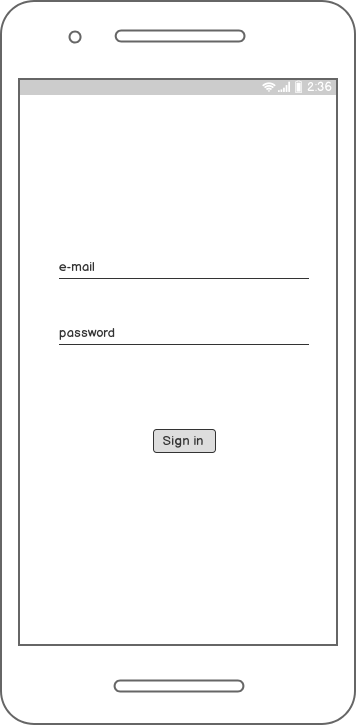
\includegraphics[width=0.3\textwidth]{Figures/3/Wireframe/login}
				\caption{หน้าจอเข้าสู่ระบบ}
				\label{Fig:หน้าจอเข้าสู่ระบบ}
			\end{figure}
			จากภาพที่ \ref{Fig:หน้าจอเข้าสู่ระบบ} แสดงหน้าจอสำหรับให้ผู้ใช้ทำการเข้าสู่ระบบ โดยจำเป็นต้องกรอกข้อมูลอีเมลและรหัสผ่านเพื่อใช้ในการเข้าสู่ระบบ
			\begin{figure}[H]
				\centering
				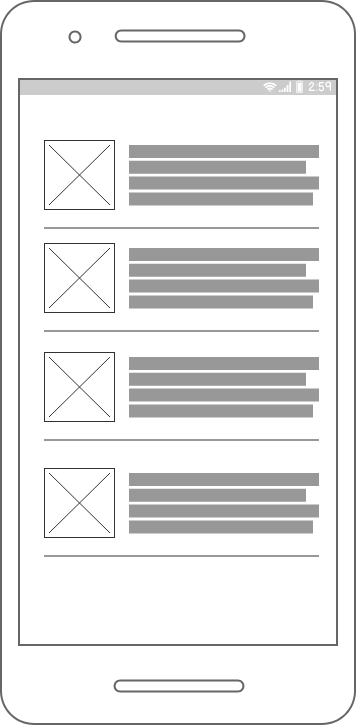
\includegraphics[width=0.3\textwidth]{Figures/3/Wireframe/feed}
				\caption{หน้าจอข่าวสารประชาสัมพันธ์}
				\label{Fig:หน้าจอข่าวสาร}
			\end{figure}
			จากภาพที่ \ref{Fig:หน้าจอข่าวสาร} แสดงหน้าจอข่าวสารหรือประชาสัมพันธ์จากเจ้าหน้าที่หรือผู้ที่เกี่ยวข้องซึ่งแสดงข้อมูลแถวรายการข่าวสารหรือประชาสัมพันธ์
			\begin{figure}[H]
				\centering
				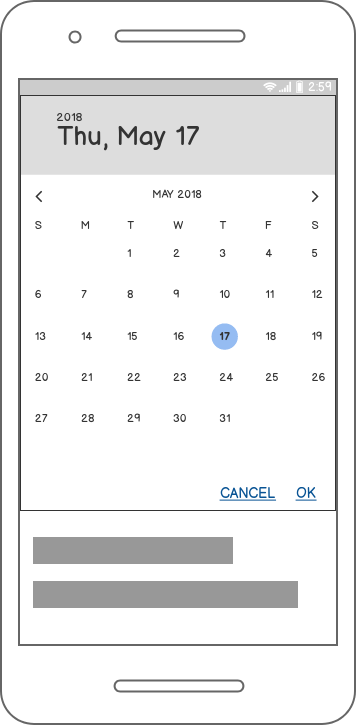
\includegraphics[width=0.3\textwidth]{Figures/3/Wireframe/calendar}
				\caption{หน้าจอปฎิทินกำหนดการ}
				\label{Fig:หน้าจอปฎิธินกำหนดการ}
			\end{figure}
			จากภาพที่ \ref{Fig:หน้าจอปฎิธินกำหนดการ} แสดงหน้าจอปฏิทินกำหนดการการดำเนินการเพื่อให้ผู้ใช้สามารถตรวจสอบกำหนดการวันที่และเวลาในการดำเนินงานของกองทุนโดยหน้าจอมีการแสดงปฏิทินและแถวรายการกำหนดการ

		\item High-fidelity wireframes \\ 
		ใช้งาน High-fidelity wireframes สำหรับการนำเสนอไอเดีย (idea) หรือรูปแบบการ Action ให้แก่ Customer เสมือนงานจริงมากที่สุด ข้อดีคือ สามารถชี้นำการใช้งานจากหน้าหนึ่งไปยังอีกหนึ่งได้ดีด้วยการทำ Motion ระหว่างหน้ารวมทั้งสามารถทำ Interaction กับผู้ใช้งานซึ่งเป็นการสร้างการโต้ตอบการใช้งานกับผู้ใช้ได้ดี
		\begin{itemize}
			\item โมบายแอปพลิเคชัน
			\begin{itemize}
				\item การออกแบบหน้าจอ splash screen 
				\begin{figure}[H]
					\centering
					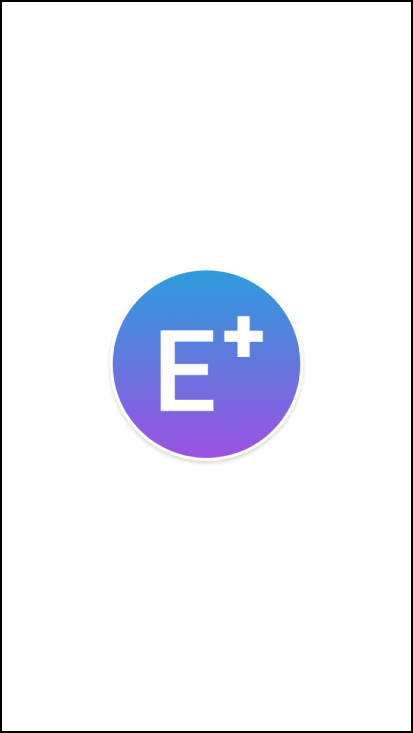
\includegraphics[width=0.3\textwidth]{Figures/3/UIMobile/splash_screen}
					\caption{หน้าจอ splash screen}
					\label{Fig:splash_screen}
				\end{figure}
				จากภาพที่ \ref{Fig:splash_screen} แสดงหน้าจอ splash screen ใช้ในการแสดงทุกครั้งที่ผู้ใช้เปิดแอปพลิเคชันโดยวัตถุประสงค์การทำงานของหน้านี้คือเพื่อใช้แสดงขณะที่แอปพลิเคชันทำการประมวลผลข้อมูลบนพื้นหลัง (Background process) เช่น การตรวจสอบสถานะการเข้าสู่ระบบของผู้ใช้คนปัจจุบัน เป็นต้น
				\item การออกแบบหน้าจอเข้าสู่ระบบ
				\begin{figure}[H]
					\centering
					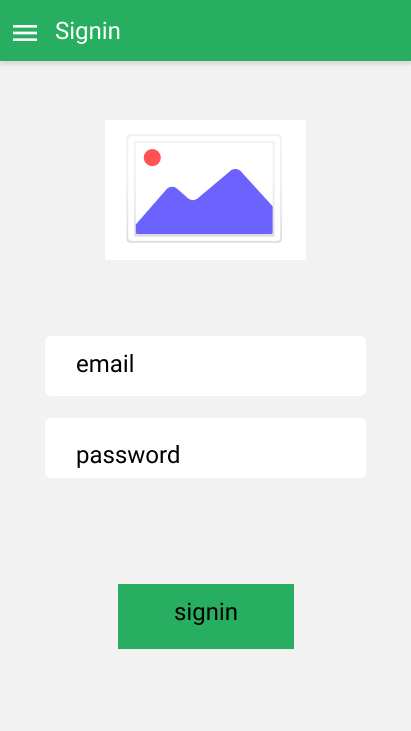
\includegraphics[width=0.3\textwidth]{Figures/3/UIMobile/sign_in}
					\caption{หน้าจอเข้าสู่ระบบ}
					\label{Fig:sign_in}
				\end{figure}
				จากภาพที่ \ref{Fig:sign_in} แสดงหน้าจอสำหรับให้ผู้ใช้ทำการเข้าสู่ระบบเมื่อผู้ใช้ยังไม่ได้ทำการเข้าสู่ระบบ โดยจำเป็นต้องกรอกข้อมูลอีเมลและรหัสผ่านเพื่อใช้ในการเข้าสู่ระบบ ซึ่งการเข้าสู่ระบบจะทำเพียงครั้งเดียวเท่านั้น เมื่อผู้ใช้เปิดการทำงานแอปพลิชันใหม่ในครั้งถัดไประบบจะระบุข้อมูลของผู้ใช้งานอัตโนมัติ
				\item การออกแบบหน้าจอสมัครสมาชิก
				\begin{figure}[H]
					\centering
					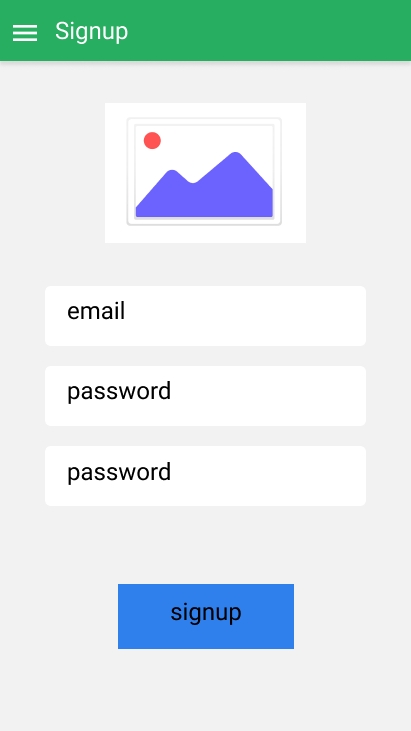
\includegraphics[width=0.3\textwidth]{Figures/3/UIMobile/sign_up}
					\caption{หน้าจอสมัครสมาชิก}
					\label{Fig:sign_up1}
				\end{figure}
				จากภาพที่ \ref{Fig:sign_up1} แสดงหน้าจอสมัครสมาชิก หากผู้ใช้ยังไม่มีบัญชีในระบบผู้ใช้งานสามารถทำการสมัครสมาชิกเพื่อเข้าใช้งานระบบได้จากหน้าสมัครสมาชิก โดยผู้ใช้จำเป็นต้องกรอกข้อมูลอีเมล รหัสผ่านและรหัสนักศึกษาในการสมัครสมาชิก
				\item การออกแบบหน้าจอข่าวสารและประชาสัมพันธ์
				\begin{figure}[H]
					\centering
					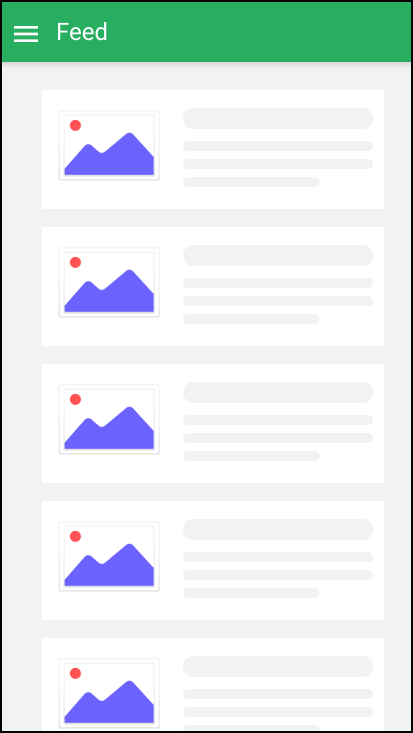
\includegraphics[width=0.3\textwidth]{Figures/3/UIMobile/home_feed}
					\caption{หน้าจอข่าวสารและประชาสัมพันธ์}
					\label{Fig:home_feed}
				\end{figure}
				จากภาพที่ \ref{Fig:home_feed} แสดงหน้าจอข่าวสารหรือประชาสัมพันธ์จากเจ้าหน้าที่หรือผู้ที่เกี่ยวข้อง
				\item การออกแบบหน้าจอเมนูนำทางหลัก 
				\begin{figure}[H]
					\centering
					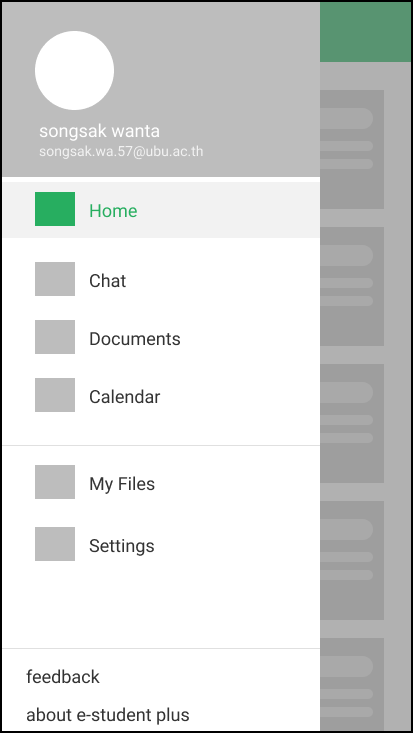
\includegraphics[width=0.3\textwidth]{Figures/3/UIMobile/home_drawer_nav}
					\caption{หน้าจอเมนูนำทางหลัก}
					\label{Fig:home_drawer_nav}
				\end{figure}
				จากภาพที่ \ref{Fig:home_drawer_nav} แสดงเมนูนำทางหลักที่ใช้นำทางผู้ใช้งานไปยังหน้าจออื่นๆ ภายในแอปพลิเคชัน
				\item การออกแบบหน้าจอปฏิทินกำหนดการการดำเนินการ
				\begin{figure}[H]
					\centering
					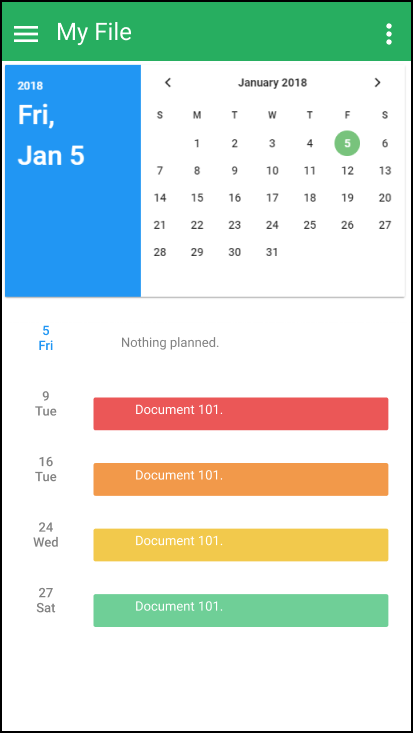
\includegraphics[width=0.3\textwidth]{Figures/3/UIMobile/home_calendar}
					\caption{หน้าจอปฏิทินกำหนดการการดำเนินการ}
					\label{Fig:home_calendar}
				\end{figure}
				จากภาพที่ \ref{Fig:home_calendar} แสดงหน้าจอปฏิทินกำหนดการการดำเนินการเพื่อให้ผู้ใช้สามารถตรวจสอบกำหนดการวันที่และเวลาในการดำเนินงานของกองทุนเงินให้กู้ยืมเพื่อการศึกษา คณะวิทยาศาสตร์ มหาวิทยาลัยอุบลราชธานี
				\item การออกแบบหน้าจอสนทนา
				\begin{figure}[H]
					\centering
					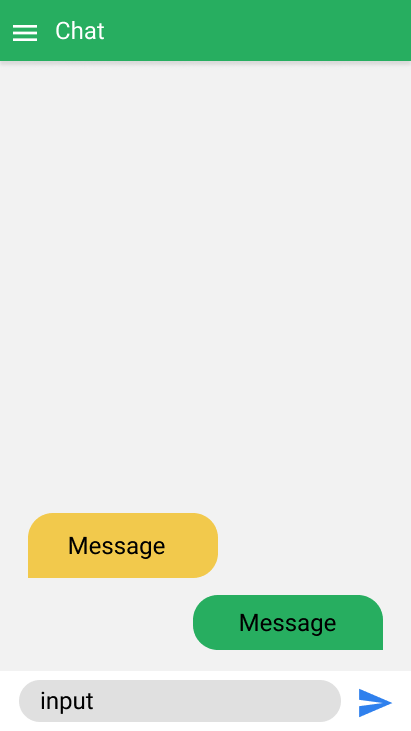
\includegraphics[width=0.3\textwidth]{Figures/3/UIMobile/home_chat}
					\caption{หน้าจอสนทนา}
					\label{Fig:home_chat}
				\end{figure}
				จากภาพที่ \ref{Fig:home_chat} นักศึกษาสามารถส่งข้อความไปยังเจ้าหน้าที่เพื่อติดต่อสอบถามข้อมูลกับทางเจ้าหน้าที่ได้โดยตรง
				\item การออกแบบหน้าจอเอกสารที่เกี่ยวข้อง
				\begin{figure}[H]
					\centering
					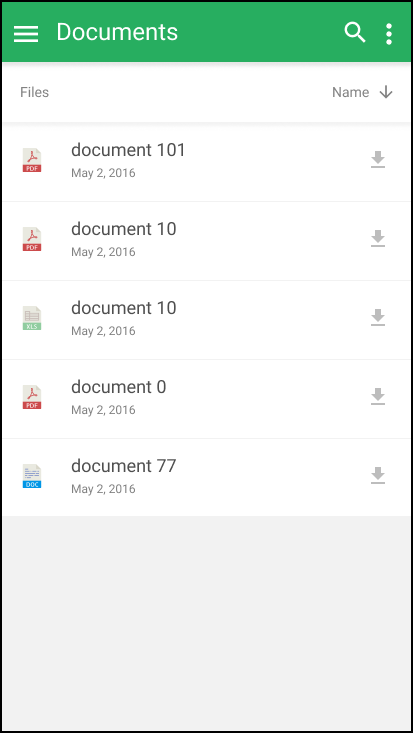
\includegraphics[width=0.3\textwidth]{Figures/3/UIMobile/home_doc}
					\caption{หน้าจอเอกสารที่เกี่ยวข้อง}
					\label{Fig:home_doc}
				\end{figure}
				จากภาพที่ \ref{Fig:home_doc} นักศึกษาสามารถดาวน์โหลดเอกสารที่เกี่ยวข้องกับกองทุนเงินให้กู้ยืมเพื่อการศึกษา คณะวิทยาศาสตร์ มหาวิทยาลัยอุบลราชธานี เช่น ข้อกำหนดและคุณสมบัติของผู้กู้ยืม เป็นต้น ซึ่งเอกสารได้ถูกอัพโหลดไว้โดยเจ้าหน้าที่
				\item การออกแบบหน้าจอจองวันที่และเวลาส่งเอกสาร
				\begin{figure}[H]
					\centering
					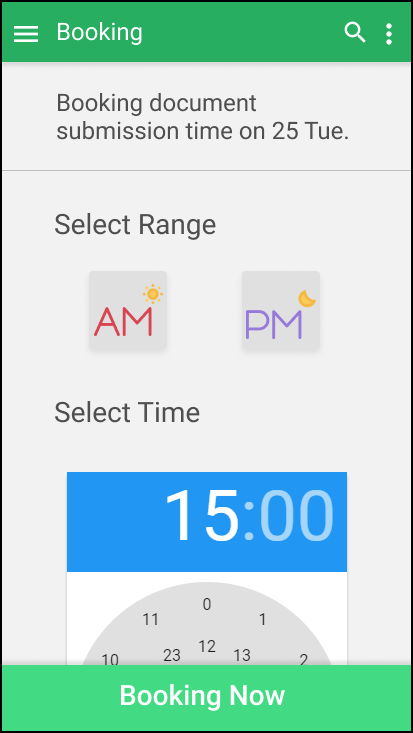
\includegraphics[width=0.3\textwidth]{Figures/3/UIMobile/home_booking}
					\caption{หน้าจอจองวันที่และเวลาส่งเอกสาร}
					\label{Fig:home_booking}
				\end{figure}
				จากภาพที่ \ref{Fig:home_booking}  เมื่อเจ้าหน้าที่ทำการเพิ่มวันที่และช่วงเวลาในการส่งเอกสาร นักศึกษาสามาจองวันที่และเวลาในการส่งเอกสารฉบับจริงของตนได้จากหน้าจอดังกล่าวโดยมีเงื่อนไขคือนักศึกษาผู้ที่จะทำการส่งเอกสารฉบับจริงจำเป็นต้องส่งภาพสำเนาเอกสารผ่านทางระบบเพื่อให้เจ้าหน้าที่ยืนยันความถูกต้องเสียก่อน
			\end{itemize}
			\item เว็บแอปพลิเคชัน
			\begin{itemize}
				\item การออกแบบหน้าจอหลัก
				\begin{figure}[H]
					\centering
					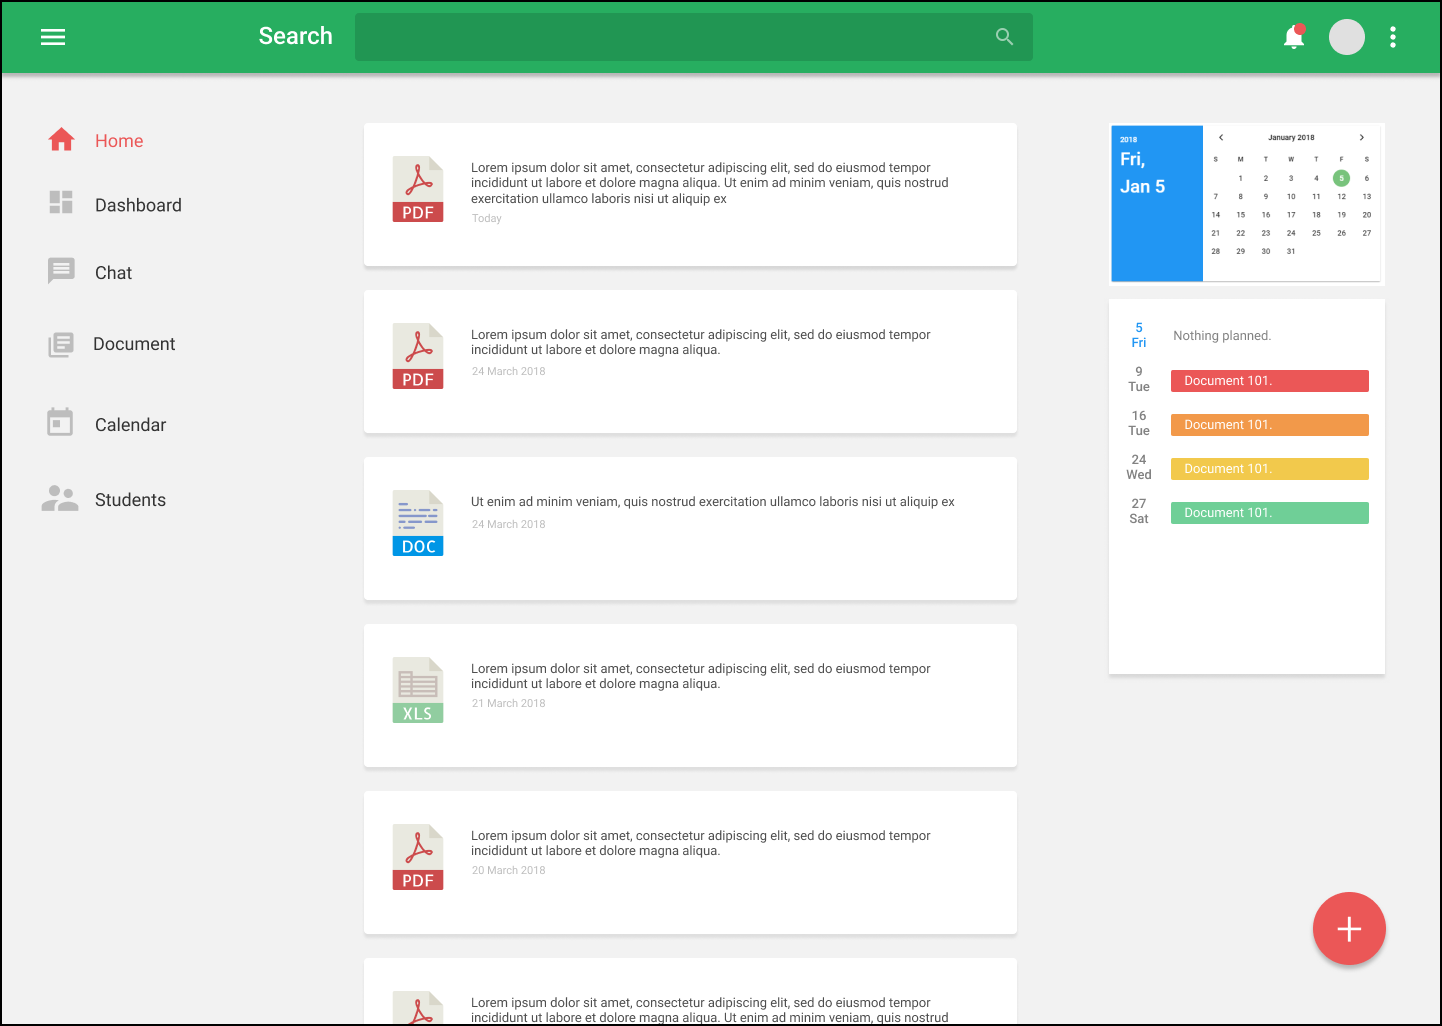
\includegraphics[width=0.8\textwidth]{Figures/3/UIWeb/Home}
					\caption{หน้าจอหลัก}
					\label{Fig:Home}
				\end{figure}
				จากภาพที่ \ref{Fig:Home}  แสดงหน้าจอหลักบนเว็บแอปพลิเคชัน  เพื่ออำนวยความสะดวกต่อเจ้าหน้าที่ ในหน้าหลักได้รวบรวมข้อมูลสรุปและเมนูเข้าถึงด่วนซึ่งแบ่งเป็น 3 ส่วนหลักได้แก่ เมนูนำทาง ข่าวสารประชาสัมพันธ์และปฏิทินกำหนดการ
				\item การออกแบบหน้าจอสนทนา
				\begin{figure}[H]
					\centering
					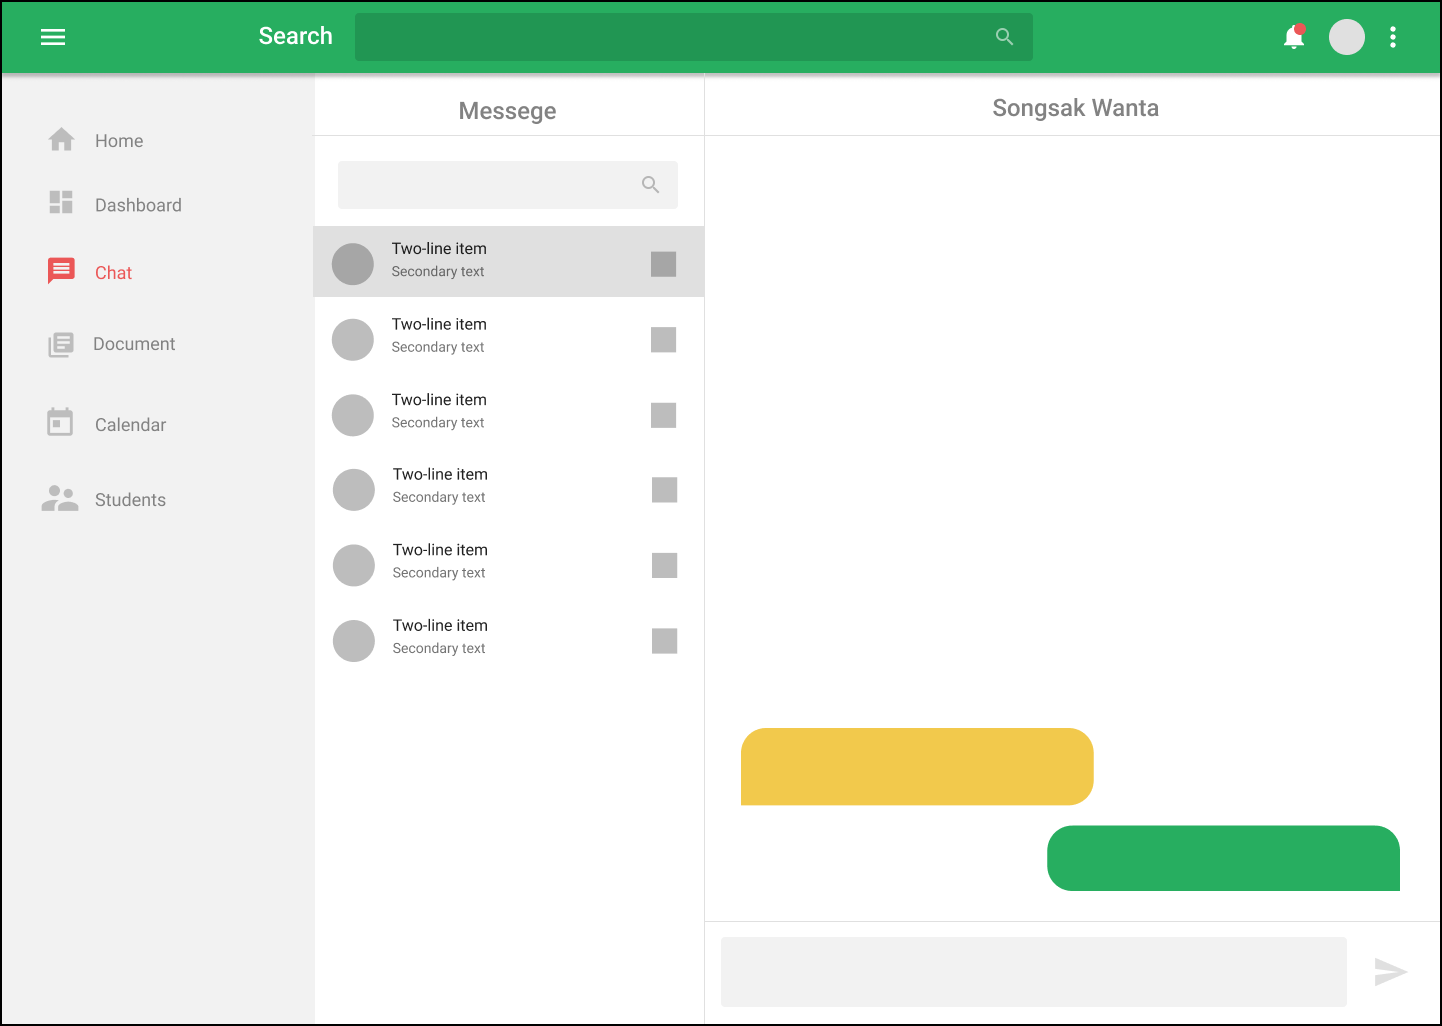
\includegraphics[width=0.8\textwidth]{Figures/3/UIWeb/Chat}
					\caption{หน้าจอสนทนา}
					\label{Fig:Chat}
				\end{figure}
				จากภาพที่ \ref{Fig:Chat}  แสดงหน้าจอสนทนามีการแสดงรายชื่อนักศึกษาและส่วนของห้องสนทนาด้วย
				\item การออกแบบหน้าจออัพโหลดเอกสาร
				\begin{figure}[H]
					\centering
					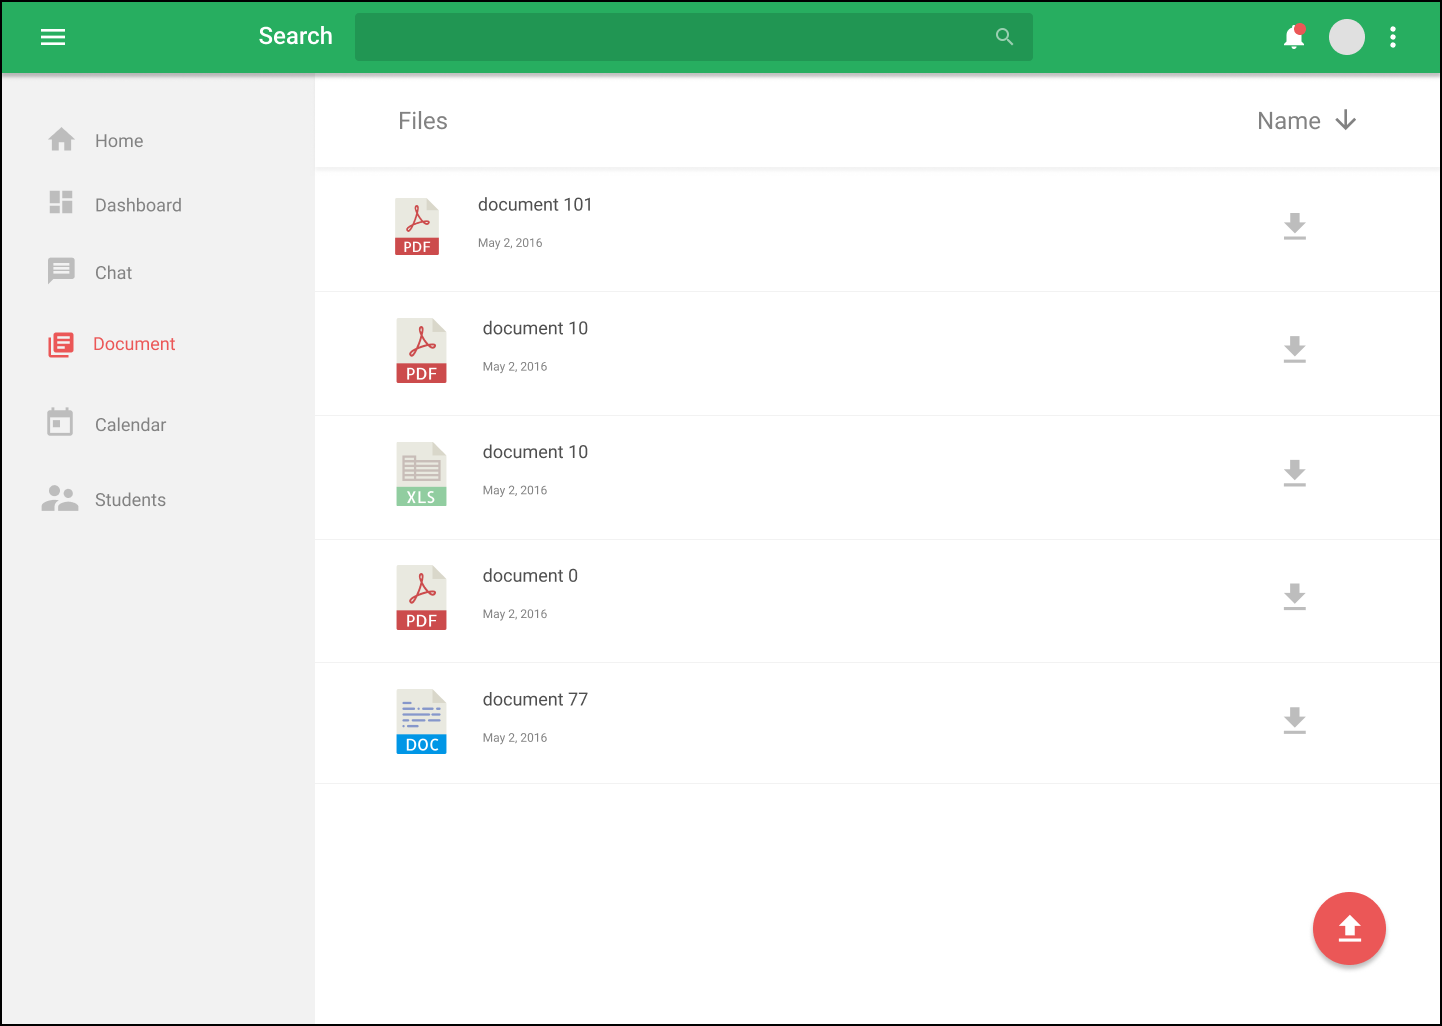
\includegraphics[width=0.8\textwidth]{Figures/3/UIWeb/Doc}
					\caption{หน้าจออัพโหลดเอกสาร}
					\label{Fig:Doc}
				\end{figure}
				จากภาพที่ \ref{Fig:Doc}  แสดงหน้าจออัพโหลดเอกสารที่เกี่ยวข้องกับกองทุนเงินให้กู้ยืมเพื่อการศึกษา คณะวิทยาศาสตร์ มหาวิทยาลัยอุบลราชธานี ทั้งนี้ผู้ที่มีสิทธิ์ในการอัพโหลดเอกสารมีเพียงเจ้าหน้าที่เท่านั้น
				\item การออกแบบหน้าจอเข้าสู่ระบบ
				\begin{figure}[H]
					\centering
					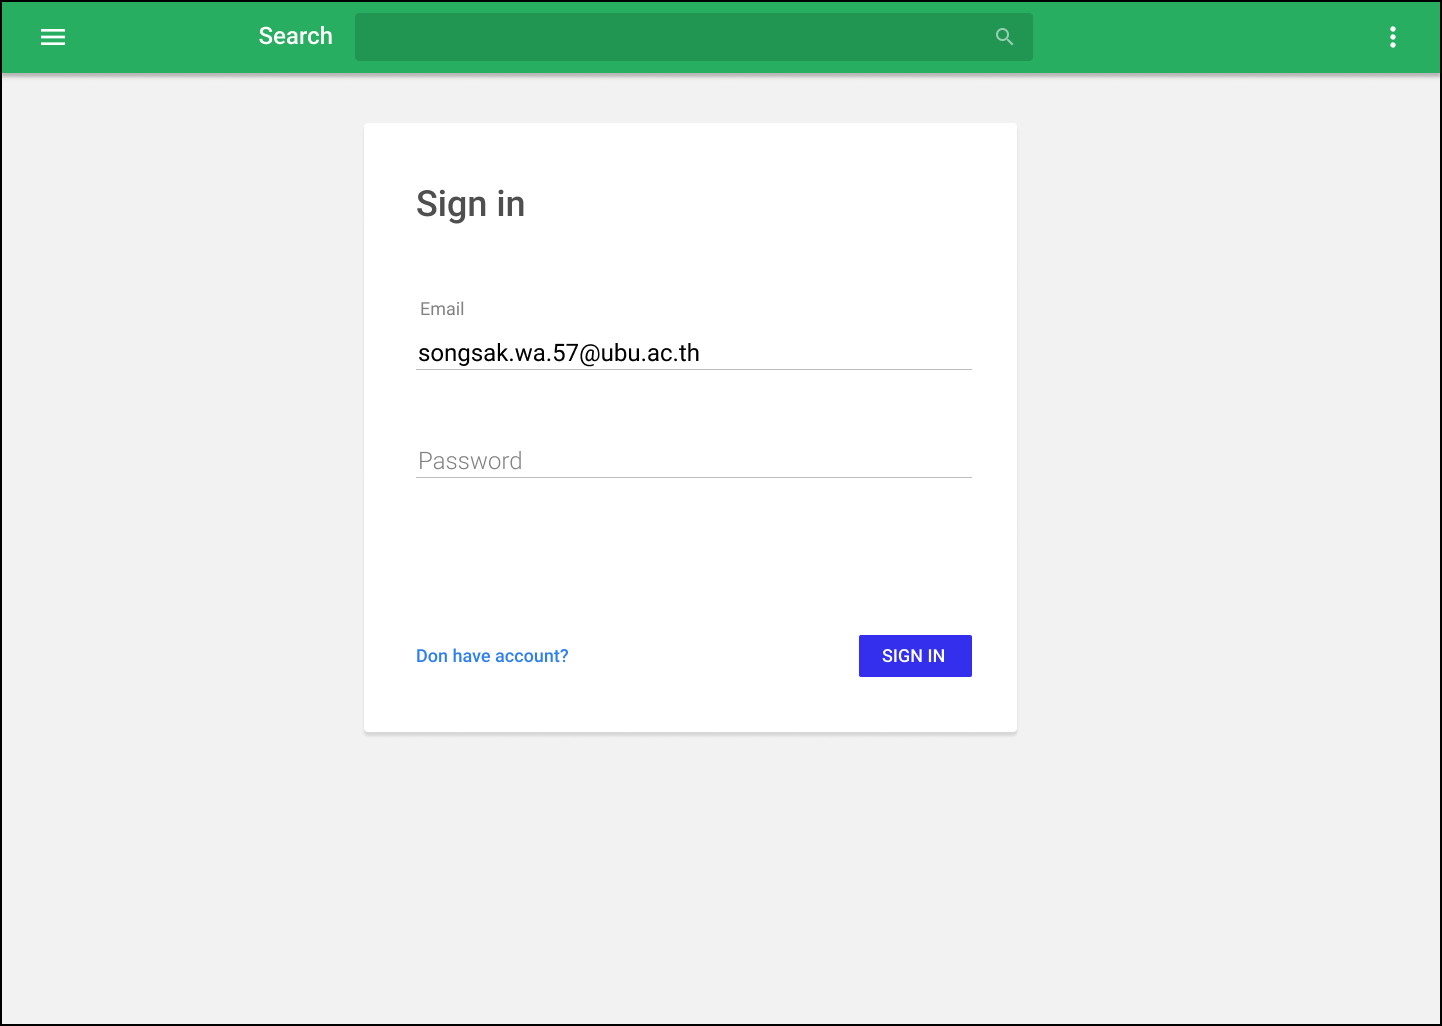
\includegraphics[width=0.8\textwidth]{Figures/3/UIWeb/Login}
					\caption{หน้าจอเข้าสู่ระบบ}
					\label{Fig:Login}
				\end{figure}
				จากภาพที่ \ref{Fig:Login} แสดงหน้าจอการเข้าสู่ระบบของผู้ใช้โดยผู้ใช้จำเป็นต้องกรอกข้อมูลอีเมลและรหัสผ่านเพื่อเข้าใช้งานระบบ
			\end{itemize}
		\end{itemize}
	\end{enumerate}
\newpage

\section{Use Case Diagram}
	Use Case Diagram เป็นแผนผังเพื่อแสดงฟังก์ชันแสดงการทำงานของระบบโดยรวม แสดงส่วนประกอบในระบบและกิจกรรมที่เกิดขึ้นในระบบซึ่งในระบบระบบกองทุนเงินให้กู้ยืมเพื่อการศึกษา คณะวิทยาศาสตร์ มหาวิทยาลัยอุบลราชธานี ผู้ใช้จำเป็นต้องเข้าสู่ระบบเพื่อใช้งานระบบ สัญลักษณ์ที่ใช้ในการเขียน Use Case Diagram แสดงในตารางที่ \ref{tab:use-case2}
	\begin{table}[H]
		\caption{สัญลักษณ์ของ Use case Diagram}
		\label{tab:use-case2}
		\begin{tabular}{|c|p{10cm}|}
		\hline
		\textbf{สัญลักษณ์} & \multicolumn{1}{c|}{\textbf{การใช้งาน}} \\ \hline
		\raisebox{-\totalheight}{Use case}
		& \setstretch{1.5} {Use case คือส่วนย่อยของระบบงาน แทนด้วยวงรีและชื่อของ Use case ภายในวงรี} \\ \hline
		\raisebox{-\totalheight}{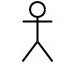
\includegraphics[height=1.5cm]{Figures/table/use-case/2}}
		& \setstretch{1.5} {Actor คือบุคคลหรือระบบงานอื่นที่ใช้งานระบบหรือได้รับประโยชน์จากระบบซึ่งอยู่ภายนอกระบบ แทนด้วยรูปคนและมีชื่อบทบาทการใช้งานระบบ} \\ \hline
		\raisebox{-\totalheight}{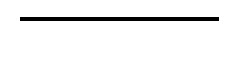
\includegraphics[width=3cm]{Figures/table/use-case/3}}
		& \setstretch{1.5} {เส้นตรงที่แสดงถึงการใช้งาน Use case ของผู้กระทำ} \\ \hline
		\raisebox{-\totalheight}{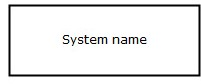
\includegraphics[width=0.3\textwidth]{Figures/table/use-case/4}}
		& \setstretch{1.5} {กรอบสี่เหลี่ยมแสดงถึงขอบเขตของระบบโดยแสดงชื่อระบบภายในหรือด้านบนกรอกสี่เหลี่ยม Use case อยู่ภายในกรอบสี่เหลี่ยม และ actor อยู่ภายนอกกรอบสี่เหลี่ยม} \\ \hline
		\raisebox{-\totalheight}{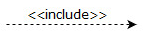
\includegraphics[width=0.3\textwidth]{Figures/table/use-case/5}}
		& \setstretch{1.5} {ความสัมพันธ์แบบ <<includes>> แสดงว่า Use case หนึ่งดำเนินการตามขั้นตอนของ Use case อื่น โดยแทนด้วยสัณลักษณ์ลูกศรเส้นประ ซึ่ง Use case ที่หางลูกศรเรียกใช้งาน Use case ที่หัวลูกศรทุกครั้งที่มีการทำงาน} \\ \hline
		\raisebox{-\totalheight}{\includegraphics[width=0.3\textwidth]{Figures/table/use-case/6}}
		& \setstretch{1.5} {ความสัมพันธ์แบบ <<extend>> แสดงว่า Use case หนึ่งดำเนินการตามขั้นตอนของ Use case อื่น โดยแทนด้วยสัญลักษณ์ลูกศรเส้นประ ซึ่ง Use case ที่หัวลูกศรเรียกใช้งาน Use case ที่หางลูกศร แต่การใช้งานไม่จำเป็นต้องเกิดขึ้นทุกครั้งขึ้นอยู่กับเงื่อนไขระหว่างการทำงาน} \\ \hline
		\end{tabular}
	\end{table}

	\begin{figure}[H]
		\includegraphics[width=1.2\textwidth]{Figures/3/usecase}
		\caption{Use Case Diagram ของระบบ XX}
		\label{Fig:usecase}
	\end{figure}
	
	\begin{table}[H]
		\centering
		\caption{อธิบาย Use Case หน้าที่ของระบบ ในภาพที่ \ref{Fig:usecase}}
		\label{tab:usecase}
		\resizebox{\totalheight}{!}{\textwidth}{%
			\begin{tabular}{|c|p{10cm}|}
				\hline
				\multicolumn{1}{|c|}{\textbf{Use Case}} & \multicolumn{1}{c|}{\textbf{คำอธิบาย}} \\ \hline
				ดูประชาสัมพันธ์ & นักศึกษาสามารถดูประชาสัมพันธ์ได้โดยไม่จำเป็นต้องทำการเข้าสู่ระบบก่อน \\ \hline
				ดูปฏิทินกำหนดการ & นักศึกษาสามารถเปิดดูปฏิทินวันที่และเวลากำหนดการของกองทุนเงินให้กู้ยืมเพื่อการศึกษา คณะวิทยาศาสตร์วิทยาลัยอุบลราชธานี โดยไม่จำเป็นต้องทำการเข้าสู่ระบบก่อน \\ \hline
				ดาวน์โหลดเอกสาร & นักศึกษาดาวน์โหลดเอกสารที่เกี่ยวข้องกับกองทุนกู้ยีมการศึกษาคณะวิทยาศาสตร์มหาวิทยาลัยอุบลราชธานีได้โดยไม่จำเป็นต้องทำการเข้าสู่ระบบก่อน \\ \hline
				ดู FAQs & หน้าแสดงรายการคำถามที่พบบ่อย \\ \hline
				จองคิวส่งเอกสาร & เมื่อนักศึกษาเข้าสู่ระบบเรียบร้อยแล้วนักศึกษา สามารถจองคิววันที่และเวลาในการส่งเอกสารฉบับจริงหลังจากที่ได้รับการตรวจสอบโดยเจ้าหน้าที่เรียบร้อยแล้ว \\ \hline
				ส่งเอกสารตรวจสอบ & นักศึกษาสามารถส่งเอกสารหน้าที่ตรวจสอบโดยการถ่ายรูปแล้วทำการอัพโหลดเข้าสู่ระบบ เมื่อเจ้าหน้าที่ตรวจสอบเรียบร้อยแล้วจะยืนยันสถานะของเอกสารอีกที \\ \hline
				สนทนา & นักศึกษาสามารถสอบถามข้อมูลของกองทุนเงินให้กู้ยืมเพื่อการศึกษา คณะวิทยาศาสตร์ มหาวิทยาลัยอุบลราชธานี ได้จากช่องสนทนา \\ \hline
				จัดการกำหนดการส่งเอกสาร & ใช้สำหรับเจ้าหน้าที่เพื่อ เพิ่ม แก้ไขหรือลบกำหนดการส่งเอกสารของนักศึกษา \\ \hline
			\end{tabular}%
		}
	\end{table}
		\begin{table}[H]
			\centering
			\caption{อธิบาย Use Case หน้าที่ของระบบ(ต่อ) ในภาพที่ \ref{tab:usecase-15}}
			\label{tab:usecase-15}
			\resizebox{\totalheight}{!}{\textwidth}{%
				\begin{tabular}{|c|p{10cm}|}
					\hline
					\multicolumn{1}{|c|}{\textbf{Use Case}} & \multicolumn{1}{c|}{\textbf{คำอธิบาย}} \\ \hline
					จัดการประชาสัมพันธ์ & ใช้สำหรับเจ้าหน้าที่เพื่อ เพิ่ม แก้ไขหรือลบประชาสัมพันธ์ \\ \hline
					จัดการปฏิทินกำหนดการ & ใช้สำหรับเจ้าหน้าที่เพื่อ เพิ่ม แก้ไขหรือลบกำหนดการการดำเนินการของกองทุน \\ \hline
					จัดการเอกสาร & ใช้สำหรับเจ้าหน้าที่เพื่อ เพิ่ม แก้ไขหรือลบเอกสารที่เกี่ยวข้องของกองทุน \\ \hline
					แจ้งเตือนนักศึกษา & ใช้เพื่อส่งแจ้งเตือนไปยังนักศึกษาเมื่อมีการเพิ่มประชาสัมพันธ์โดยเจ้าหน้าที่ \\ \hline
				\end{tabular}%
			}
		\end{table}
	% Please add the following required packages to your document preamble:
	% \usepackage{graphicx}
	\begin{table}[H]
		\centering
		\caption{Use Case ดูประชาสัมพันธ์}
		\label{tab:usecase}
		\resizebox{\totalheight}{!}{\textwidth}{%
			\begin{tabular}{|p{10cm}|p{10cm}|}
				\hline
				\multicolumn{1}{|c|}{\textbf{Use Case Title : ดูประชาสัมพันธ์}} & \multicolumn{1}{c|}{\textbf{Use case Id : 1 }} \\ \hline
				\multicolumn{2}{|p{\linewidth}|}{Primary Actor : นักศึกษา} \\ \hline
			    \multicolumn{2}{|p{\linewidth}|}{Stakeholder Actor : เจ้าหน้าที่} \\ \hline
			    \multicolumn{2}{|p{\linewidth}|}{Main Flow : นักศึกษาดูประชาสัมพันธ์โดยไม่จำเป็นต้องเข้าสู่ระบบ} \\ \hline
			    \multicolumn{2}{|p{\linewidth}|}{Exceptional Flow ที่ 1 : หากผู้ใช้ไม่เชื่อมต่ออินเทอร์เน็ต จะไม่สามารถดูประชาสัมพันธ์ได้} \\ \hline
			\end{tabular}%
		}
	\end{table}
	\begin{table}[H]
		\centering
		\caption{Use Case ดูปฏิทินกำหนดการ}
		\label{tab:usecase}
		\resizebox{\totalheight}{!}{\columnwidth}{%
			\begin{tabular}{|p{7cm}|p{7cm}|}
				\hline
				\multicolumn{1}{|c|}{\textbf{Use Case Title : ดูปฏิทินกำหนดการ}} & \textbf{Use case Id : 2 } \\ \hline
				\multicolumn{2}{|l|}{Primary Actor : นักศึกษา} \\ \hline
				\multicolumn{2}{|l|}{Stakeholder Actor : เจ้าหน้าที่} \\ \hline
				\multicolumn{2}{|p{\linewidth}|}{Main Flow : นักศึกษาสามารถเปิดดูปฏิทินวันที่และเวลากำหนดการของกองทุนเงินให้กู้ยืมเพื่อการศึกษา  คณะวิทยาศาสตร์ มหาวิทยาลัยอุบลราชธานี ไม่จำเป็นต้องเข้าสู่ระบบ} \\ \hline
				\multicolumn{2}{|p{\linewidth}|}{Exceptional Flow ที่ 1 : หากผู้ใช้ไม่เชื่อมต่ออินเทอร์เน็ต จะไม่สามารถดูปฏิทินกำหนดการได้} \\ \hline
			\end{tabular}%
		}
	\end{table}

	\begin{table}[H]
		\centering
		\caption{Use Case ดาวน์โหลดเอกสาร}
		\label{tab:usecase}
		\resizebox{\totalheight}{!}{\textwidth}{%
			\begin{tabular}{|p{7cm}|p{7cm}|}
				\hline
				\multicolumn{1}{|c|}{\textbf{Use Case Title : ดาวน์โหลดเอกสาร}} & \textbf{Use case Id : 3 } \\ \hline
				\multicolumn{2}{|l|}{Primary Actor : นักศึกษา} \\ \hline
				\multicolumn{2}{|l|}{Stakeholder Actor : เจ้าหน้าที่} \\ \hline
				\multicolumn{2}{|p{\linewidth}|}{Main Flow : นักศึกษาดาวน์โหลดเอกสารที่เกี่ยวข้องกับกองทุนกู้ยีมการศึกษา
				คณะวิทยาศาสตร์มหาวิทยาลัยอุบลราชธานีได้ไม่จำเป็นต้องเข้าสู่ระบบ} \\ \hline
				\multicolumn{2}{|p{\linewidth}|}{Exceptional Flow ที่ 1 : หากผู้ใช้ไม่เชื่อมต่ออินเทอร์เน็ต จะไม่สามารดาวน์โหลดเอกสารที่เกี่ยวข้องกับกองทุนได้} \\ \hline
				\multicolumn{2}{|p{\linewidth}|}{Exceptional Flow ที่ 2 : หากผู้ใช้โมบายแอปพลิเคชันไม่เปิดสิทธิ์การอ่านและเขียนไฟล์บนความจำสำรอง จะไม่สามารถดาวน์โหลดเอกสารที่เกี่ยวข้องกับกองทุนได้} \\ \hline
			\end{tabular}%
		}
		\end{table}
		
		\begin{table}[H]
			\centering
			\caption{Use Case ดู FAQs}
			\label{tab:usecase}
			\resizebox{\totalheight}{!}{\textwidth}{%
				\begin{tabular}{|p{10cm}|p{10cm}|}
					\hline
					\multicolumn{1}{|c|}{\textbf{Use Case Title : ดู FAQs}} & \multicolumn{1}{c|}{\textbf{Use case Id : 4 }} \\ \hline
					\multicolumn{2}{|l|}{Primary Actor : นักศึกษา} \\ \hline
					\multicolumn{2}{|l|}{Stakeholder Actor : เจ้าหน้าที่} \\ \hline
					\multicolumn{2}{|p{\linewidth}|}{Main Flow : ใช้เพื่อแสดงรายการคำถามที่พบบ่อย } \\ \hline
					\multicolumn{2}{|p{\linewidth}|}{Exceptional Flow ที่ 1 : หากผู้ใช้ไม่เชื่อมต่ออินเทอร์เน็ต จะไม่สามารถดูคำถามที่พบบ่อยได้} \\ \hline
				\end{tabular}%
			}
		\end{table}
		
		\begin{table}[H]
			\centering
			\caption{Use Case จองคิวส่งเอกสาร}
			\label{tab:usecase}
			\resizebox{\totalheight}{!}{\textwidth}{%
				\begin{tabular}{|c|p{10cm}|}
					\hline
					\multicolumn{1}{|c|}{\textbf{Use Case Title : จองคิวส่งเอกสาร}} & \multicolumn{1}{c|}{\textbf{Use case Id : 5 }} \\ \hline
					\multicolumn{2}{|l|}{Primary Actor : นักศึกษา} \\ \hline
					\multicolumn{2}{|l|}{Stakeholder Actor : เจ้าหน้าที่} \\ \hline
					\multicolumn{2}{|p{\linewidth}|}{Main Flow :เมื่อนักศึกษาเข้าสู่ระบบเรียบร้อยแล้วนักศึกษา สามารถจองคิววันที่และเวลาในการส่งเอกสารฉบับจริงหลังจากที่ได้รับการตรวจสอบโดยเจ้าหน้าที่เรียบร้อยแล้ว } \\ \hline
					\multicolumn{2}{|p{\linewidth}|}{Exceptional Flow ที่ 1 : หากผู้ใช้ไม่เชื่อมต่ออินเทอร์เน็ต จะไม่สามารถจองคิวส่งเอกสารได้} \\ \hline
				\end{tabular}%
			}
		\end{table}
	
		\begin{table}[H]
			\centering
			\caption{Use Case ส่งเอกสารตรวจสอบ}
			\label{tab:usecase}
			\resizebox{\totalheight}{!}{\textwidth}{%
				\begin{tabular}{|c|p{10cm}|}
					\hline
					\multicolumn{1}{|c|}{\textbf{Use Case Title : ส่งเอกสารตรวจสอบ}} & \multicolumn{1}{c|}{\textbf{Use case Id : 6 }} \\ \hline
					\multicolumn{2}{|l|}{Primary Actor : นักศึกษา} \\ \hline
					\multicolumn{2}{|l|}{Stakeholder Actor : เจ้าหน้าที่} \\ \hline
					\multicolumn{2}{|p{\linewidth}|}{Main Flow : นักศึกษาสามารถส่งเอกสารหน้าที่ตรวจสอบโดยการถ่ายรูปแล้วทำการอัพโหลดเข้าสู่ระบบ เมื่อเจ้าหน้าที่ตรวจสอบเรียบร้อยแล้วจะยืนยันสถานะของเอกสารอีกที } \\ \hline
					\multicolumn{2}{|p{\linewidth}|}{Exceptional Flow ที่ 1 : หากผู้ใช้ไม่เชื่อมต่ออินเทอร์เน็ต จะไม่สามารถส่งเอกสารตรวจสอบได้} \\ \hline
					\multicolumn{2}{|p{\linewidth}|}{Exceptional Flow ที่ 1 : หากผู้ใช้โมบายแอปพลิเคชันไม่เปิดสิทธิ์ใช้งานกล้อง จะไม่สามารถถ่ายภาพเพื่อส่งเอกสารตรวจสอบได้} \\ \hline
				\end{tabular}%
			}
		\end{table}	
		
		\begin{table}[H]
			\centering
			\caption{Use Case สนทนา}
			\label{tab:usecase}
			\resizebox{\totalheight}{!}{\textwidth}{%
				\begin{tabular}{|c|p{10cm}|}
					\hline
					\multicolumn{1}{|c|}{\textbf{Use Case Title : สนทนา}} & \multicolumn{1}{c|}{\textbf{Use case Id : 7 }} \\ \hline
					\multicolumn{2}{|l|}{Primary Actor : นักศึกษา} \\ \hline
					\multicolumn{2}{|l|}{Stakeholder Actor : เจ้าหน้าที่} \\ \hline
					\multicolumn{2}{|p{\linewidth}|}{Main Flow : เมื่อนักศึกษาเข้าสู่ระบบแล้วจะสามารถสอบถามข้อมูลของกองทุนเงินให้กู้ยืมเพื่อการศึกษา คณะวิทยาศาสตร์ มหาวิทยาลัยอุบลราชธานี ได้จากช่องสนทนา} \\ \hline
					\multicolumn{2}{|p{\linewidth}|}{Exceptional Flow ที่ 1 : หากผู้ใช้ไม่เชื่อมต่ออินเทอร์เน็ต จะไม่สามารถสนทนาได้} \\ \hline
				\end{tabular}%
			}
		\end{table}	
%		\begin{table}[H]
%			\centering
%			\caption{Use Case สมัครสมาชิก}
%			\label{tab:usecase}
%			\resizebox{\totalheight}{!}{\textwidth}{%
%				\begin{tabular}{|c|p{10cm}|}
%					\hline
%					\multicolumn{1}{|c|}{\textbf{Use Case Title : สมัครสมาชิก}} & \multicolumn{1}{c|}{\textbf{Use case Id : 8 }} \\ \hline
%					\multicolumn{2}{|l|}{Primary Actor : นักศึกษา} \\ \hline
%					\multicolumn{2}{|l|}{Stakeholder Actor : -} \\ \hline
%					\multicolumn{2}{|p{\linewidth}|}{Main Flow : เมื่อนักศึกษาต้องการใช้งานระบบทั้งหมดของกองทุนจำเป็นต้องเข้าสู่ระบบก่อน หากยังไม่มีบัญชีสามารถสมัครได้โดยต้องกรอกข้อมูลอีเมลและรหัสผ่าน} \\ \hline
%					\multicolumn{2}{|p{\linewidth}|}{Exceptional Flow ที่ 1 : หากผู้ใช้ไม่เชื่อมต่ออินเทอร์เน็ต จะไม่สามารถสมัครสมาชิกได้} \\ \hline
%				\end{tabular}%
%			}
%		\end{table}	
%		 \begin{table}[H]
%		 	\centering
%		 	\caption{Use Case เข้าสู่ระบบ}
%		 	\label{tab:usecase}
%		 	\resizebox{\totalheight}{!}{\textwidth}{%
%		 		\begin{tabular}{|c|p{10cm}|}
%		 			\hline
%		 			\multicolumn{1}{|c|}{\textbf{Use Case Title : เข้าสู่ระบบ}} & \multicolumn{1}{c|}{\textbf{Use case Id : 9 }} \\ \hline
%		 			\multicolumn{2}{|l|}{Primary Actor : นักศึกษา} \\ \hline
%		 			\multicolumn{2}{|l|}{Stakeholder Actor : -} \\ \hline
%		 			\multicolumn{2}{|p{\linewidth}|}{Main Flow : เมื่อนักศึกษาต้องการใช้งานระบบทั้งหมดของกองทุนจำเป็นต้องเข้าสู่ระบบก่อนโดยต้องกรอกข้อมูลอีเมลและรหัสผ่าน} \\ \hline
%		 			\multicolumn{2}{|p{\linewidth}|}{Exceptional Flow ที่ 1 : หากผู้ใช้ไม่เชื่อมต่ออินเทอร์เน็ต จะไม่สามารถเข้าสู่ระบบได้} \\ \hline
%		 		\end{tabular}%
%		 	}
%		 \end{table}	
		  \begin{table}[H]
		  	\centering
		  	\caption{Use Case จัดการกำหนดการส่งเอกสาร}
		  	\label{tab:usecase}
		  	\resizebox{\totalheight}{!}{\textwidth}{%
		  		\begin{tabular}{|c|p{10cm}|}
		  			\hline
		  			\multicolumn{1}{|c|}{\textbf{Use Case Title : จัดการกำหนดการส่งเอกสาร}} & \multicolumn{1}{c|}{\textbf{Use case Id : 10 }} \\ \hline
		  			\multicolumn{2}{|l|}{Primary Actor : เจ้าหน้าที่} \\ \hline
		  			\multicolumn{2}{|l|}{Stakeholder Actor : -} \\ \hline
		  			\multicolumn{2}{|p{\linewidth}|}{Main Flow : เจ้าหน้าที่ เพิ่ม แก้ไขหรือลบกำหนดการส่งเอกสารของนักศึกษา} \\ \hline
		  			\multicolumn{2}{|p{\linewidth}|}{Exceptional Flow ที่ 1 : หากเจ้าหน้าที่ไม่เชื่อมต่ออินเทอร์เน็ต จะไม่สามารถ เพิ่ม แก้ไขหรือลบกำหนดการส่งเอกสารของนักศึกษาได้} \\ \hline
		  		\end{tabular}%
		  	}
		  \end{table}	
		  \begin{table}[H]
			    	\centering
			    	\caption{Use Case จัดการประชาสัมพันธ์}
			    	\label{tab:usecase}
			    	\resizebox{\totalheight}{!}{\textwidth}{%
			    		\begin{tabular}{|c|p{10cm}|}
			    			\hline
			    			\multicolumn{1}{|c|}{\textbf{Use Case Title : จัดการประชาสัมพันธ์}} & \multicolumn{1}{c|}{\textbf{Use case Id : 11 }} \\ \hline
			    			\multicolumn{2}{|l|}{Primary Actor : เจ้าหน้าที่} \\ \hline
			    			\multicolumn{2}{|l|}{Stakeholder Actor : -} \\ \hline
			    			\multicolumn{2}{|p{\linewidth}|}{Main Flow : เจ้าหน้าที่ เพิ่ม แก้ไขหรือลบปฏิทินกำหนดการในระบบได้} \\ \hline
			    			\multicolumn{2}{|p{\linewidth}|}{Exceptional Flow ที่ 1 : หากเจ้าหน้าที่ไม่เชื่อมต่ออินเทอร์เน็ต จะไม่สามารถ เพิ่ม แก้ไขหรือลบปฏิทินกำหนดการได้} \\ \hline
			    		\end{tabular}%
			    	}
		  \end{table}	
		    \begin{table}[H]
		    	\centering
		    	\caption{Use Case จัดการปฏิทินกำหนดการ}
		    	\label{tab:usecase}
		    	\resizebox{\totalheight}{!}{\textwidth}{%
		    		\begin{tabular}{|c|p{10cm}|}
		    			\hline
		    			\multicolumn{1}{|c|}{\textbf{Use Case Title : จัดการปฏิทินกำหนดการ}} & \multicolumn{1}{c|}{\textbf{Use case Id : 12 }} \\ \hline
		    			\multicolumn{2}{|l|}{Primary Actor : เจ้าหน้าที่} \\ \hline
		    			\multicolumn{2}{|l|}{Stakeholder Actor : -} \\ \hline
		    			\multicolumn{2}{|p{\linewidth}|}{Main Flow : เจ้าหน้าที่ เพิ่ม แก้ไขหรือลบปฏิทินกำหนดการได้} \\ \hline
		    			\multicolumn{2}{|p{\linewidth}|}{Exceptional Flow ที่ 1 : หากเจ้าหน้าที่ไม่เชื่อมต่ออินเทอร์เน็ต จะไม่สามารถ เพิ่ม แก้ไขหรือลบปฏิทินกำหนดการได้} \\ \hline
		    		\end{tabular}%
		    	}
		    \end{table}	
		   \begin{table}[H]
		   	\centering
		   	\caption{Use Case จัดการเอกสาร}
		   	\label{tab:usecase}
		   	\resizebox{\totalheight}{!}{\textwidth}{%
		   		\begin{tabular}{|c|p{10cm}|}
		   			\hline
		   			\multicolumn{1}{|c|}{\textbf{Use Case Title : จัดการเอกสาร}} & \multicolumn{1}{c|}{\textbf{Use case Id : 13 }} \\ \hline
		   			\multicolumn{2}{|l|}{Primary Actor : เจ้าหน้าที่} \\ \hline
		   			\multicolumn{2}{|l|}{Stakeholder Actor : -} \\ \hline
		   			\multicolumn{2}{|p{\linewidth}|}{Main Flow : เจ้าหน้าที่ เพิ่ม แก้ไขหรือลบเอกสารที่เกี่ยวข้องกับกองทุนได้} \\ \hline
		   			\multicolumn{2}{|p{\linewidth}|}{Exceptional Flow ที่ 1 : หากเจ้าหน้าที่ไม่เชื่อมต่ออินเทอร์เน็ต จะไม่สามารถ เพิ่ม แก้ไขหรือลบเอกสารที่เกี่ยวข้องกับกองทุนได้} \\ \hline
		   		\end{tabular}%
		   	}
		   \end{table}	
			  \begin{table}[H]
			  	\centering
			  	\caption{Use Case แจ้งเตือนนักศึกษา}
			  	\label{tab:usecase}
			  	\resizebox{\totalheight}{!}{\textwidth}{%
			  		\begin{tabular}{|c|p{10cm}|}
			  			\hline
			  			\multicolumn{1}{|c|}{\textbf{Use Case Title : แจ้งเตือนนักศึกษา}} & \multicolumn{1}{c|}{\textbf{Use case Id : 14 }} \\ \hline
			  			\multicolumn{2}{|l|}{Primary Actor : เจ้าหน้าที่} \\ \hline
			  			\multicolumn{2}{|l|}{Stakeholder Actor : -} \\ \hline
			  			\multicolumn{2}{|p{\linewidth}|}{Main Flow : แจ้งเตือนไปยังนักศึกษาเมื่อมีการเพิ่มประชาสัมพันธ์โดยเจ้าหน้าที่} \\ \hline
			  			\multicolumn{2}{|p{\linewidth}|}{Exceptional Flow ที่ 1 : หากนักศึกษาที่ไม่เชื่อมต่ออินเทอร์เน็ต จะไม่สามารถรับแจ้งเตือนเมื่อมีการเพิ่มประชาสัมพันธ์โดยเจ้าหน้าที่} \\ \hline
			  		\end{tabular}%
			  	}
			  \end{table}	
\newpage

\section{Class Diagram}
	Class Diagram คือแผนภาพที่ใช้แสดงคลาสและความสัมพันธ์ในแบบต่างๆ ระหว่างคลาส สัญลักษณ์ที่ใช้ในการเขียน Class Diagram แสดงในตารางที่ \ref{tab:class2} 
	\begin{center}
	\begin{table}[H]
		\centering
		\caption{สัญลักษณ์ของ Class Diagram}
		\label{tab:class2}
		\begin{tabular}{|c|p{10cm}|}
			\hline
			\textbf{สัญลักษณ์} & \multicolumn{1}{c|}{\textbf{การใช้งาน}} \\ \hline
			\raisebox{-\totalheight}{\includegraphics[width=0.3\textwidth]{Figures/table/class/11}}
			& \setstretch{1.5} {คลาส สัญลักษณ์แทนด้วยสี่เหลี่ยมแบ่งเป็น 3 ส่วน 
				ส่วนบน เป็นชื่อของ class ส่วนกลาง เป็นชื่อ Attribute และส่วนล่างเป็น Operation Name หรือ Method ใช้สำหรับเขียนฟังก์ชันในการทำงานของคลาสนั้น ๆ
				ชนิดของ Visibility ของ Method และ Attribute
				แบ่งเป็น 3 ชนิด ได้แก่
				\begin{enumerate}
					\item Public แทนสัญลักษณ์ด้วยเครื่องหมายบวก (+)
					\item Private แทนสัญลักษณ์ด้วยเครื่องหมายลบ (-)
					\item Protected แทนสัญลักษณ์ด้วยเครื่องหมายชาร์ป (#)
				\end{enumerate}
			} \\ \hline
			\raisebox{-\totalheight}{\includegraphics[width=0.3\textwidth]{Figures/table/class/1}}
			& \setstretch{1.5} {Dependency Relationship หมายความว่า คลาสที่อยู่ฝั่งต้นลูกศรสามารถเรียกใช้คลาสที่อยู่ฝั่งหัวลูกศร}
			\\ \hline
			\raisebox{-\totalheight}{\includegraphics[width=0.35\textwidth]{Figures/3/Class/aggre}}
			& \setstretch{1.5} {Composition Relationship เป็นความสัมพันธ์ระหว่างออบเจ็กต์หรือคลาสแบบขึ้นต่อกันและมีความเกี่ยวข้องกันเสมอ} \\ \hline
			\raisebox{-\totalheight}{\includegraphics[width=0.3\textwidth]{Figures/3/Class/implement}}
			& \setstretch{1.5} {Realization Relationship เป็นความสัมพันธ์ระหว่าง Object หรือ Class ในลักษณะของการสืบทอดคุณสมบัติจาก Class หนึ่ง (Super class) ไปยังอีก Class หนึ่ง (Subclass)} \\ \hline
			\raisebox{-\totalheight}{\includegraphics[width=50,height=50]{Figures/table/class/connector}}
			& \setstretch{1.5} {Connector เป็นสัญลักษณ์แทนด้วยรูปห้าเหลี่ยมและมีชื่ออยู่ตรงกลาง จะสร้างสัญลักษณ์นี้ไว้เมื่อต้องการเชื่อมต่อคลาสที่อยู่คนละหน้า} \\ \hline
		\end{tabular}
	\end{table}
	\end{center}

\newpage
  %IMAGE of class
	Class Diagram แสดงความสัมพันธ์ในรูปแบบต่างๆ ระหว่างคลาสของแอปพลิเคชันระบบกองทุนเงินให้กู้ยืมเพื่อการศึกษา คณะวิทยาศาสตร์ มหาวิทยาลัยอุบลราชธานี อธิบายได้ตามภาพที่ \ref{Fig:MainActivity20C} ดังต่อไปนี้
	\begin{figure}[H]
		\includegraphics[width=1.0\columnwidth]{Figures/3/Class/MainActivity}
		\caption{Class Diagram ของแอปพลิเคชันระบบ XX}
		\label{Fig:MainActivity20C}
	\end{figure}
	\begin{figure}[H]
		\includegraphics[width=1.0\columnwidth]{Figures/3/Class/Feed}
		\caption{Class Diagram ของแอปพลิเคชันระบบ XX}
		\label{Fig:FeedC}
	\end{figure}
\begin{sidewaysfigure}
	\begin{figure}[H]
		\includegraphics[width=1.0\columnwidth]{Figures/3/Class/Doc}
		\caption{Class Diagram ของแอปพลิเคชันระบบ XX}
		\label{Fig:DocC}
	\end{figure}
\end{sidewaysfigure}
	\begin{figure}[H]
		\includegraphics[width=\columnwidth]{Figures/3/Class/Submit}
		\caption{Class Diagram ของแอปพลิเคชันระบบ XX}
		\label{Fig:SubmitC}
	\end{figure}
	\begin{figure}[H]
		\includegraphics[width=1.0\columnwidth]{Figures/3/Class/UserChat}
		\caption{Class Diagram ของแอปพลิเคชันระบบ XX}
		\label{Fig:UserChatC}
	\end{figure}

	% TABLE of class
\newpage	
	จากรูปภาพที่ \ref{Fig:MainActivity20C} สามารถอธิบายแผนภาพ Class Diagram ได้ดังนี้
	\begin{table}[H]
		\centering
		\caption{อธิบาย Class Diagram ของคลาสพื้นฐานของระบบ}
		\label{tab:class}
		\begin{tabular}{|c|p{10cm}|}
			\hline
			\textbf{Class Diagram} & \multicolumn{1}{c|}{\textbf{คำอธิบาย}} \\ \hline
			\raisebox{-\totalheight}{MainApplication}
			& \setstretch{1.5} {คลาส MainApplication จะถูกเรียกใช้งานทุกครั้งเมื่อผู้ใช้เปิดแอปพลิเคชัน โดยวัตถุประสงค์การทำงานของคลาสนี้คือ เพื่อใช้จัดการทรัพยากรที่จำเป็นสำหรับการใช้งานในคลาสอื่น ๆ } \\ \hline
			\raisebox{-\totalheight}{SplashScreenActivity}
			& \setstretch{1.5} {คลาส SplashScreenActivity จะถูกเรียกใช้งานทุกครั้งเมื่อผู้ใช้เปิดแอปพลิเคชัน โดยวัตถุประสงค์การทำงานของคลาสคือ เพื่อใช้ตรวจสอบสถานะการเข้าสู่ระบบของผู้ใช้} \\ \hline
			\raisebox{-\totalheight}{MainActivity}
			& \setstretch{1.5} {คลาส MainActivity เป็นคลาสหลักที่ใช้ในการทำงานของแอปพลิเคชันโดยการทำงานของคลาสนี้เน้นไปที่การสร้าง Fragment เพื่อใช้แสดงข้อมูลต่าง ๆ โดยองค์ประกอบการทำงานของคลาสนี้ประกอบบไปด้วยสองส่วนหลักๆ ได้แก่ เมนูนำทาง Drawer และ Fragment Container} \\ \hline
			\raisebox{-\totalheight}{SignInActivity}
			& \setstretch{1.5} {คลาส SignInActivity เป็นคลาสที่ใช้เพื่อให้สมาชิกที่ได้ลงทะเบียนกับระบบเข้าสู่ระบบเพื่อใช้งานบริการต่าง ๆ จากระบบ} \\ \hline
	\end{tabular}
\end{table}

\newpage
จากรูปภาพที่ \ref{Fig:FeedC} สามารถอธิบายแผนภาพ Class Diagram ได้ดังนี้
\begin{table}[H]
	\centering
	\caption{อธิบาย Class Diagram ของส่วนของการแสดงข่าวสาร}
	\label{tab:class}
	\begin{tabular}{|c|p{10cm}|}
		\hline
		\textbf{Class Diagram} & \multicolumn{1}{c|}{\textbf{คำอธิบาย}} \\ \hline
		\raisebox{-\totalheight}{FeedFragment}
		& \setstretch{1.5} {คลาส FeedFragment เป็นคลาสหลักที่ใช้ในการแสดงข้อมูลข่าวสาร มีการทำงานหลักคือสืบค้นฐานข้อมูลจากไฟร์เบสเพื่อนำมาแสดง} \\ \hline
		\raisebox{-\totalheight}{FeedItemAdapter}
		& \setstretch{1.5} {คลาส FeedItemAdapter เป็นคลาสที่มีหน้าที่ในการแปลงชุดข้อมูลที่ได้จากคลาส FeedFragment แล้วคืนค่ากลับเป็นลิสต์รายการของชุดข้อมูลนั้น ๆ} \\ \hline
		\raisebox{-\totalheight}{Post}
		& \setstretch{1.5} {คลาส Post เป็นคลาสโมเดลที่กำหนดค่าต่างๆที่จำเป็นสำหรับใช้ในการสร้างลิสต์รายการของคลาส FeedItemAdapter} \\ \hline
		\raisebox{-\totalheight}{PostDetailActivity}
		& \setstretch{1.5} {คลาส PostDetailActivity เป็นคลาสที่มีหน้าที่ในการแสดงข้อมูลรายละเอียดของข่าวสารแต่ละแถวที่ได้รับจากหน้า FeedFragment ที่จะส่งข้อมูลเมื่อผู้ใช้กดที่แถวรายการข่าวสาร} \\ \hline
		\raisebox{-\totalheight}{RecyclerViewClickListener}
		& \setstretch{1.5} {คลาส RecyclerViewClickListener เป็นคลาสอินเทอร์เฟส(Interface)ที่ใช้ในการสร้างแม่แบบเมื่อคลาสใด ๆ ต้องการใช้งานสำหรับการรับค่าเมื่อผู้ใช้กดแถวในลิสต์รายการ คลาสลูกที่ทำการสืบทอดคุณสมบัติจะสามารถรับข้อมูลตำแหน่งแถวที่ผู้ใช้กดบนลิสต์รายการได้} \\ \hline
	\end{tabular}
\end{table}

\newpage
จากรูปภาพที่ \ref{Fig:DocC} สามารถอธิบายแผนภาพ Class Diagram ได้ดังนี้
\begin{table}[H]
	\centering
	\caption{อธิบาย Class Diagram ของส่วนของการแสดงรายการเอกสารในระบบ}
	\label{tab:class}
	\begin{tabular}{|c|p{10cm}|}
		\hline
		\textbf{Class Diagram} & \multicolumn{1}{c|}{\textbf{คำอธิบาย}} \\ \hline
		\raisebox{-\totalheight}{DocumentsFragment}
		& \setstretch{1.5} {คลาส DocumentsFragment เป็นคลาสที่ใช้ในการแสดงข้อมูลเอกสารที่ถูกอัพโหลดเข้าสู่ระบบโดยเจ้าหน้าที่ซึ่งจะถูกแสดงเป็นลิสต์รายการ} \\ \hline
		\raisebox{-\totalheight}{DocItemAdapter}
		& \setstretch{1.5} {คลาส DocItemAdapter เป็นคลาสที่มีหน้าที่ในการแปลงชุดข้อมูลที่ได้รับจากคลาส DocumentsFragment เป็นลิสต์รายการแล้วคืนกลับไปยังคลาส DocumentsFragment} \\ \hline
		\raisebox{-\totalheight}{Doc}
		& \setstretch{1.5} {คลาส Doc เป็นคลาสโมเดลที่กำหนดค่าต่าง ๆ ที่จำเป็นสำหรับใช้ในการสร้างลิสต์รายการของคลาส DocItemAdapter} \\ \hline
		\raisebox{-\totalheight}{RecyclerViewClickListener}
		& \setstretch{1.5} {คลาส RecyclerViewClickListener เป็นคลาสอินเทอร์เฟสที่ใช้ในการสร้างแม่แบบเมื่อคลาสใด ๆ ต้องการใช้งานสำหรับการรับค่าเมื่อผู้ใช้กดแถวในลิสต์รายการ คลาสลูกที่ทำการสืบทอดคุณสมบัติจะสามารถรับข้อมูลตำแหน่งแถวที่ผู้ใช้กดบนลิสต์รายการได้} \\ \hline
	\end{tabular}
\end{table}

\newpage
จากรูปภาพที่ \ref{Fig:SubmitC} สามารถอธิบายแผนภาพ Class Diagram ได้ดังนี้
\begin{table}[H]
	\centering
	\caption{อธิบาย Class Diagram ของส่วนของการส่งสำเนาเอกสาร}
	\label{tab:class}
	\begin{tabular}{|c|p{10cm}|}
		\hline
		\textbf{Class Diagram} & \multicolumn{1}{c|}{\textbf{คำอธิบาย}} \\ \hline
		\raisebox{-\totalheight}{SubmitFragment}
		& \setstretch{1.5} {คลาส SubmitFragment เป็นคลาสที่ใช้ในการแสดงหน้าจอส่งสำเนาเอกสาร โดยมีการดำเนินการภายในคลาสหลัก ๆ ได้แก่ การถ่ายภาพ แปลงภาพและบันทึกภาพเข้าสู่ระบบ} \\ \hline
	\end{tabular}
\end{table}

จากรูปภาพที่ \ref{Fig:UserChatC} สามารถอธิบายแผนภาพ Class Diagram ได้ดังนี้
\begin{table}[H]
	\centering
	\caption{อธิบาย Class Diagram ของส่วนของการสนทนา}
	\label{tab:class}
	\begin{tabular}{|c|p{10cm}|}
		\hline
		\textbf{Class Diagram} & \multicolumn{1}{c|}{\textbf{คำอธิบาย}} \\ \hline
		\raisebox{-\totalheight}{UserChatFragment}
		& \setstretch{1.5} {คลาส UserChatFragment เป็นคลาสที่ใช้ในการแสดงหน้าจอสนทนาสำหรับนักศึกษา เพื่อติดต่อสอบถามข้อมูลกับเจ้าหน้าที่ มีการสืบค้นข้อมูลประวัติการสนทนาเพื่อส่งไปแปลงเป็นข้อมูลลิสต์รายการที่คลาส MessagesListAdapter} \\ \hline
		\raisebox{-\totalheight}{MessagesListAdapter}
		& \setstretch{1.5} {คลาส MessagesListAdapter เป็นคลาสที่ใช้ในการแปลงชุดข้อมูลที่ได้รับจากคลาส UserChatFragment เป็นลิสต์รายการแล้วทำการคืนค่าลิสต์รายการที่ได้กลับไปยังคลาส UserChatFragment} \\ \hline 
		\raisebox{-\totalheight}{MessagesList}
		& \setstretch{1.5} {คลาส MessagesList เป็นคลาสที่ใช้ในการจัดเก็บข้อมูลภายในคลาส UserChatFragment หลังจากที่ได้ทำการสืบค้นข้อมูลการสนทนาจากไฟร์เบสเพื่อส่งไปยังคลาส MessagesListAdapter} \\ \hline
		\raisebox{-\totalheight}{RecyclerViewClickListener}
		& \setstretch{1.5} {คลาส RecyclerViewClickListener เป็นคลาสอินเทอร์เฟสที่ใช้ในการสร้างแม่แบบเมื่อคลาสใด ๆ ต้องการใช้งานสำหรับการรับค่าเมื่อผู้ใช้กดแถวในลิสต์รายการ คลาสลูกที่ทำการสืบทอดคุณสมบัติจะสามารถรับข้อมูลตำแหน่งแถวที่ผู้ใช้กดบนลิสต์รายการได้} \\ \hline
	\end{tabular}
\end{table}

\newpage
\section{Sequence Diagram}
	Sequence Diagram เป็น Diagram ที่แสดงขั้นตอนการทำงานของแต่ละ Use Case ระหว่าง Object ต่างๆ ที่ส่งข้อความถึงกันและกัน โดย Sequence Diagram จะช่วยให้มองเห็นการทำงานของภาพรวมของระบบ ส่วนประกอบสัญลักษณ์ที่ใช้ในการเขียน Sequence Diagram 
	แสดงดังตารางที่ \ref{tab:Sequences}
	
	\begin{table}[H]
		\centering
		\caption{สัญลักษณ์ของ Sequence Diagram}
		\label{tab:Sequences}
		\begin{tabular}{| c	| p{10cm} |}
		\hline
		\textbf{สัญลักษณ์} & \multicolumn{1}{c|}{\textbf{การใช้งาน}} \\ \hline
		\raisebox{-\totalheight}{\includegraphics[width=0.17\textwidth]{Figures/table/Sequence/Sequence1}}
		& \setstretch{1.5} {Class แสดงถึงการทำงานของ Use Case ในการส่งหรือรับข้อความ แทนด้วยสัญลักษณ์สี่เหลี่ยมมีชื่อคลาสอยู่ภายใน} \\ \hline
		\raisebox{-\totalheight}{\includegraphics[height=0.08\textheight]{Figures/table/Sequence/Sequence2}}
		& \setstretch{1.5} {Lifeline หรือเส้นอายุขัย แสดงช่วงเวลาตั้งแต่เริ่มสร้าง object ในคลาสนั้น จนกระทั่ง object นั้นถูกทำลาย สัญลักษณ์แทนด้วยเส้นประ} \\ \hline
		\raisebox{-\totalheight}{\includegraphics[height=0.08\textheight]{Figures/table/Sequence/Sequence3}}
		& \setstretch{1.5} {Focus of control หรือจุดควบคุม เป็นจุดควบคุมที่ object ใช้ทำการส่งหรือรับข้อความ สัญลักษณ์แทนด้วยสี่เหลี่ยม} \\ \hline
		\raisebox{-\totalheight}{\includegraphics[width=0.3\textwidth]{Figures/table/Sequence/Sequence4}}
		& \setstretch{1.5} {Message คือ ข้อความที่รับส่งระหว่าง Object สัญลักษณ์แทนด้วยลูกศรและประกอบด้วย 2 ส่วน คือ ข้อมูล (Data) และฟังก์ชัน (Function)} \\ \hline
		\raisebox{-\totalheight}{\includegraphics[width=0.3\textwidth]{Figures/table/Sequence/Sequence5}}
		& \setstretch{1.5} {Return Message เป็นข้อมูลที่ส่งกลับหลังจากทำงานเสร็จ} \\ \hline
		\raisebox{-\totalheight}{\includegraphics[height=0.08\textheight]{Figures/3/selfcall}}
		& \setstretch{1.5} {Self call เป็นการเรียกฟังชันก์การทำงานภายในตัวเอง} \\ \hline
		\raisebox{-\totalheight}{\includegraphics[height=0.1\textheight,width=0.3\textwidth]{Figures/3/frame}}
		& \setstretch{1.5} {สร้างกรอบการทำงานของโปรแกรม เพื่อให้รู้ขอบเขตของการทำงานเช่น ลูป(loop)} \\ \hline
		\end{tabular}
	\end{table}
%
%	Sequence Diagram ที่ใช้อธิบายการทำงานของระบบกองทุนเงินให้กู้ยืมเพื่อการศึกษา คณะวิทยสศาสตร์ มหาวิทยาลัยอุบลราชธานี มีรายละเอียดดังต่อไปนี้

\newpage
	\begin{landscape}
	\begin{figure}[H]
		\centering
		\includegraphics[width=0.95\columnwidth]
		{Figures/3/Sequence/feed}
		\caption{Sequence Diagram การแสดงข่าวสาร}
		\label{Fig:Sequence-feed}
	\end{figure}
  \end{landscape}

	จากภาพที่ \ref{Fig:Sequence-feed} สามารถอธิบายแผนภาพ Sequence Diagram แสดงข่าวสาร ได้ดังนี้ เมื่อ
	ผู้ใช้เปิดโปรแกรมระบบจะเรียกใช้เมธอด onCreate() ที่คลาส MainActivity ระบบจะทำการสร้าง
	Fragment ขึ้นมาโดยใช้เมธอด onCreate() ที่คลาส FeedFragment เมื่อ FeedFragment ถูกติดตั้งบน MainActivity เมธอด callData() จะสืบค้นข้อมูลจากฐานข้อมูลบน Firebase FireStore และส่งข้อมูลที่ได้ไปแปลงที่คลาส FeedItemAdapter โดยมีการคืนค่าเป็นข้อมูลข่าวสารแต่ละแถวและในขั้นตอนสุดท้ายคลาส FeedFragment จะทำการแสดงรายการข้อมูลข่าวสารทั้งหมดออกทางหน้าจอ หากผู้ใช้มีการกดเลือกข่าวสารบางแถวคลาส FeedFragment จะทำการเรียกใช้ PostDetailActivity เพื่อแสดงรายละเอียดข้อมูลข่าวสารของแถวที่ถูกเลือก
	\begin{sidewaysfigure}
	\begin{figure}[H]
		\centering
		\includegraphics[width=0.8\columnwidth]
		{Figures/3/Sequence/calendar}
		\caption{Sequence Diagram การแสดงปฏิทินกำหนดการ}
		\label{Fig:Sequence-calendar}
	\end{figure}
	\end{sidewaysfigure}
	\newpage
	จากภาพที่ \ref{Fig:Sequence-calendar} สามารถอธิบายแผนภาพ Sequence Diagram แสดงปฏิทินกำหนดการ ได้ดังนี้ เมื่อ
	ผู้ใช้เปิดโปรแกรมระบบจะเรียกใช้เมธอด onCreate() ที่คลาส MainActivity ระบบจะทำการสร้าง
	Fragment ขึ้นมาโดยใช้เมธอด onCreate() ที่คลาส ScheduleFragment เมื่อ ScheduleFragment ถูกติดตั้งบน MainActivity เมธอด callData() จะสืบค้นข้อมูลกำหนดการของวันปัจจุบันจากฐานข้อมูลบน Firebase FireStore และส่งข้อมูลที่ได้ไปแปลงที่คลาส Schedule-ItemAdapter โดยมีการคืนค่าเป็นข้อมูลกำหนดการแต่ละแถวและในขั้นตอนสุดท้ายคลาส Schedule-Fragment จะทำการแสดงรายการกำหนดการวันปัจจุบันออกทางหน้าจอ หากผู้ใช้มีการกดเลือกวันที่ที่ต้องการทราบกำหนดการจากปฏิทินคลาส ScheduleFragment จะทำการเรียกใช้ callData() อีกครั้งโดยสืบค้นข้อมูลกำหนดการของวันที่ถูกเลือกจากฐานข้อมูลบน Firebase FireStore และส่งข้อมูลที่ได้ไปแปลงที่คลาส ScheduleItemAdapter โดยมีการคืนค่าเป็นข้อมูลแต่กำหนดการละแถวและในขั้นตอนสุดท้ายคลาส ScheduleFragment จะทำการแสดงรายการกำหนดการวันที่ผู้ใช้เลือกออกทางหน้าจอ

	\begin{sidewaysfigure}
	\begin{figure}[H]
		\centering
		\includegraphics[width=0.8\columnwidth]
		{Figures/3/Sequence/doc}
		\caption{Sequence Diagram การแสดงดาวน์โหลดเอกสาร}
		\label{Fig:Sequence-doc}
	\end{figure}
	\end{sidewaysfigure}
	\newpage
	จากภาพที่ \ref{Fig:Sequence-doc} สามารถอธิบายแผนภาพ Sequence Diagram แสดงดาวน์โหลดเอกสาร ได้ดังนี้ เมื่อผู้ใช้เปิดโปรแกรมระบบจะเรียกใช้เมธอด onCreate() ที่คลาส MainActivity ระบบจะทำการสร้าง
	Fragment ขึ้นมาโดยใช้เมธอด onCreate() ที่คลาส DocumentsFragment เมื่อ DocumentsFragment ถูกติดตั้งบน MainActivity เมธอด initInstances() จะสืบค้นข้อมูลเอกสารทั้งหมดจากฐานข้อมูลบน Firebase FireStore และส่งข้อมูลที่ได้ไปแปลงที่คลาส DocItem-Adapter โดยมีการคืนค่าเป็นข้อมูลเอกสารแต่ละแถวและในขั้นตอนสุดท้ายคลาส Documents-Fragment จะทำการแสดงรายการกำหนดการวันปัจจุบันออกทางหน้าจอ

	\begin{sidewaysfigure}
	\begin{figure}[H]
		\centering
		\includegraphics[width=0.8\columnwidth]
		{Figures/3/Sequence/chat}
		\caption{Sequence Diagram การแสดงบทสนทนา}
		\label{Fig:Sequence-chat}
	\end{figure}
	\end{sidewaysfigure}
	\newpage
	จากภาพที่ \ref{Fig:Sequence-chat} สามารถอธิบายแผนภาพ Sequence Diagram แสดงการสนทานา ได้ดังนี้ เมื่อผู้ใช้เปิดโปรแกรมระบบจะเรียกใช้เมธอด onCreate() ที่คลาส MainActivity ระบบจะทำการสร้าง
	Fragment ขึ้นมาโดยใช้เมธอด onCreate() ที่คลาส UserChatFragment เมื่อ UserChatFrag-ment ถูกติดตั้งบน MainActivity เมธอด getMessage() จะสืบค้นข้อมูลประวัติการสนทนาของผู้ใช้คนปัจจุบันทั้งหมดจากฐานข้อมูลบน Firebase FireStore และส่งข้อมูลที่ได้ไปแปลงที่คลาส MessagesListAdapter โดยมีการคืนค่าเป็นข้อมูลรายการประวัติการสนทนาทั้งหมดและในขั้นตอนสุดท้ายคลาส User-ChatFragment จะทำการแสดงรายการประวัติการสนทนาทั้งหมดออกทางหน้าจอ เมื่อผู้ใช้พิมพ์ข้อความและกดปุ่มส่งระบบจะเรียกให้เมธอด send() เพื่อทำการบันทึกข้อมูลไว้บน Firebase FireStore และทำการแสดงข้อมูลรายการประวัติการสนทนาทั้งหมดที่ถูกอัพเดท

	\begin{sidewaysfigure}
	\begin{figure}[H]
		\centering
		\includegraphics[width=0.8\columnwidth]
		{Figures/3/Sequence/submit}
		\caption{Sequence Diagram แสดงส่งเอกสารตรวจสอบ}
		\label{Fig:Sequence-submit}
	\end{figure}
	\end{sidewaysfigure}
	\newpage
	จากภาพที่ \ref{Fig:Sequence-submit} สามารถอธิบายแผนภาพ Sequence Diagram แสดงส่งเอกสารตรวจสอบ ได้ดังนี้ เมื่อผู้ใช้เปิดโปรแกรมระบบจะเรียกใช้เมธอด onCreate() ที่คลาส MainActivity ระบบจะทำการสร้าง
	Fragment ขึ้นมาโดยใช้เมธอด onCreate() ที่คลาส SubmitFragment เมื่อ Submit-Fragment ถูกติดตั้งบน MainActivity เมธอด initInstances() จะถูกเรียกเพื่อสร้างหน้าจอแสงดผลเมื่อผู้ใช้กดปุ่มถ่ายรูประบบจะเรียกใช้ไลบรารี่ ScanConstants เพื่อถ่ายภาพเอกสารและรอให้ผู้ใช้ถ่ายครบทั้งสองแผ่นจึงจะแสดงปุ่มกดส่งเอกสารเพื่อตรวจสอบ
\newpage	 
	
\section{โครงสร้างฐานข้อมูลไฟร์เบส(Firebase Database Stucture)}
Firebase Database นั้นเป็น Database แบบ NoSQL และเป็น JSON database ที่มีโครงสร้างที่เป็น Key และ Value จัดเก็บข้อมูลในลักษณะโหนด หากต้องการเรียกงานจะเรียกใช้โดย
การท่องไปยังโหนดที่ต้องการ ส่วนประกอบสัญลักษณ์ที่ใช้ในการเขียนโครงสร้างฐานข้อมูลแบบ Firebase
แสดงดังตารางที่ \ref{tab:DB}

\begin{table}[H]
	\centering
	\caption{สัญลักษณ์ของโครงสร้างฐานข้อมูลแบบ Firebase}
	\label{tab:DB}
	\begin{tabular}{| c	| p{10cm} |}
		\hline
		\textbf{สัญลักษณ์} & \multicolumn{1}{c|}{\textbf{คำอธิบาย}} \\ \hline
		\raisebox{-\totalheight}{\includegraphics[width=0.1\textwidth]{Figures/3/DB/dbroot}}
		& \setstretch{1.5} {Database เป็นการเรียกชื่อแทนโหนด(Node)บนสุดที่ใช้ในการเก็บข้อมูล} \\ \hline
		\raisebox{-\totalheight}{\includegraphics[width=0.1\textwidth]{Figures/3/DB/dbcollection}}
		& \setstretch{1.5} {Collection เป็นการเรียกชื่อแทนของการเก็บหลาย ๆ เอกสารไว้ด้วยกัน} \\ \hline
		\raisebox{-\totalheight}{\includegraphics[width=0.1\textwidth]{Figures/3/DB/dbdoc}}
		& \setstretch{1.5} {Document เป็นการเรียกชื่อแทนหน่วยการเก็บของข้อมูลใน Cloud Firestore ภายในจะประกอบไปด้วย ชื่อของ Document  ชื่อของคีย์ (key) และ ค่าข้อมูล (value) โดยชื่อของ Document ห้ามซ้ำกัน ซึ่งใน Cloud Firestore สามารถระบุประเภทของข้อมูลได้ 9 ประเภทได้แก่ boolean, number, string, geo point, timestamp, array, object, reference และ null} \\ \hline
	\end{tabular}
\end{table}
	\begin{figure}[H]
	\centering
	\includegraphics[width=0.7\columnwidth]
	{Figures/3/DB/DB1}
	\caption{โครงสร้างฐานข้อมูลแบบ Firebase}
	\label{Fig:DB1}
	\end{figure}

	\begin{figure}[H]
	\centering
	\includegraphics[width=0.9\columnwidth]
	{Figures/3/DB/DB2}
	\caption{โครงสร้างฐานข้อมูลแบบ Firebase(ต่อ)}
	\label{Fig:DB2}
\end{figure}
	\begin{figure}[H]
	\centering
	\includegraphics[width=0.55\columnwidth]
	{Figures/3/DB/DB3}
	\caption{โครงสร้างฐานข้อมูลแบบ Firebase(ต่อ)}
	\label{Fig:DB3}
\end{figure}
	\begin{figure}[H]
	\centering
	\includegraphics[width=0.7\columnwidth]
	{Figures/3/DB/DB4}
	\caption{โครงสร้างฐานข้อมูลแบบ Firebase(ต่อ)}
	\label{Fig:DB4}
\end{figure}

\newpage
จากรูที่ \ref{Fig:DB1}-\ref{Fig:DB4} สามารถอธิบายโครงสร้างของข้อมูลได้ดังนี้
\begin{figure}[H]
\centering
\includegraphics[width=0.5\columnwidth]
{Figures/3/DB/nodePost}
\caption{โหนดเก็บข้อมูลประกาศ}
\label{Fig:DB4}
\end{figure}
\begin{table}[H]
	\centering
	\caption{อธิบายโหนดที่ใช้เก็บข้อมูลประกาศ}
	\label{my-label1}
	\begin{tabular}{|c|p{10cm}|}
		\hline
		\multicolumn{1}{|c|}{\textbf{Key}} & \multicolumn{1}{c|}{\textbf{คำอธิบาย}} \\ \hline
		Posts & โหนดสำหรับเก็บข้อมูลประกาศทั้งหมด \\ \hline
		Post &  สำหรับเก็บข้อมูลแต่ละประกาศ \\ \hline
		title & สำหรับเก็บชื่อหัวข้อประกาศ \\ \hline
		description & สำหรับเก็บรายละเอียดประกาศ  \\ \hline
		collection & สำหรับเก็บประเภทของประกาศได้แก่ สาธารณะและเฉพาะบุคคล \\ \hline
		fileURL & สำหรับเก็บ url ของเอกสารแนบประกาศ \\ \hline
		id & สำหรับเก็บรหัสของประกาศ \\ \hline
		time & สำหรับเก็บเวลาที่ประกาศ \\ \hline
	\end{tabular}
\end{table}

\newpage
\begin{figure}[H]
	\centering
	\includegraphics[width=0.5\columnwidth]
	{Figures/3/DB/nodeDoc}
	\caption{โหนดเก็บข้อมูลเอกสารที่เกี่ยวข้อง}
	\label{Fig:DB4}
\end{figure}
\begin{table}[H]
	\centering
	\caption{อธิบายโหนดที่ใช้เก็บข้อมูลเอกสารที่เกี่ยวข้อง}
	\label{my-label1}
	\begin{tabular}{|c|p{10cm}|}
		\hline
		\multicolumn{1}{|c|}{\textbf{Key}} & \multicolumn{1}{c|}{\textbf{คำอธิบาย}} \\ \hline
		Docs & โหนดสำหรับเก็บข้อมูลของเอกสารที่เกี่ยวข้องทั้งหมด \\ \hline
		Doc &  สำหรับเก็บข้อมูลเอกสารแต่ละฉบับ \\ \hline
		title & สำหรับเก็บชื่อหัวเรื่องของเอกสาร \\ \hline
		description & สำหรับเก็บรายละเอียดของเอกสาร \\ \hline
		fileType & สำหรับนามสกุลไฟล์เอกสาร เช่น .pdf .png เป็นต้น \\ \hline
		fileURL & สำหรับเก็บ url ของเอกสาร\\ \hline
		time & สำหรับเก็บเวลาที่ถูกอัพโหลดเข้าสู่ระบบโดยเจ้าหน้าที่\\ \hline
	\end{tabular}
\end{table}

\newpage
\begin{figure}[H]
	\centering
	\includegraphics[width=0.4\columnwidth]
	{Figures/3/DB/nodeChat}
	\caption{โหนดเก็บข้อมูลประวัติการสนทนา}
	\label{Fig:DB4}
\end{figure}
\begin{table}[H]
	\centering
	\caption{อธิบายโหนดที่ใช้เก็บข้อมูลประวัติการสนทนา}
	\label{my-label1}
	\begin{tabular}{|c|p{10cm}|}
		\hline
		\multicolumn{1}{|c|}{\textbf{Key}} & \multicolumn{1}{c|}{\textbf{คำอธิบาย}} \\ \hline
		Chats & โหนดสำหรับเก็บข้อมูลประวัติการสนทนาทั้งหมด \\ \hline
		User\_id &  สำหรับเก็บประวัติการสนทนาของผู้ใช้แต่ละคน \\ \hline
		Messages & สำหรับเก็บประวัติการสนทนาทั้งหมดของผู้ใช้ \\ \hline
		Message & สำหรับเก็บข้อมูลของแต่ละข้อความ \\ \hline
		message & สำหรับเก็บข้อความ \\ \hline
		name & สำหรับเก็บชื่อของผู้ส่งข้อความ\\ \hline
		photo & สำหรับเก็บ url รูปภาพของผู้ส่งข้อความ\\ \hline
		senderId & สำหรับเก็บรหัสของผู้ส่งข้อความ\\ \hline
		time & สำหรับเก็บเวลาที่ข้อความถูกส่ง\\ \hline
	\end{tabular}
\end{table}

\newpage
\begin{figure}[H]
	\centering
	\includegraphics[width=0.5\columnwidth]
	{Figures/3/DB/nodeEvent}
	\caption{โหนดเก็บข้อมูลกำหนดการ}
	\label{Fig:DB4}
\end{figure}
\begin{table}[H]
	\centering
	\caption{อธิบายโหนดที่ใช้เก็บข้อมูลกำหนดการ}
	\label{my-label1}
	\begin{tabular}{|c|p{10cm}|}
		\hline
		\multicolumn{1}{|c|}{\textbf{Key}} & \multicolumn{1}{c|}{\textbf{คำอธิบาย}} \\ \hline
		Events & โหนดสำหรับเก็บข้อมูลของกำหนดการทั้งหมด \\ \hline
		Event & สำหรับเก็บข้อมูลของแต่ละกำหนดการ \\ \hline
		title & สำหรับเก็บชื่อหัวข้อของกำหนดการ \\ \hline
		description & สำหรับเก็บรายละเอียดของกำหนดการ\\ \hline
		time & สำหรับเก็บเวลาของกำหนดการ\\ \hline
	\end{tabular}
\end{table}

\newpage
\begin{figure}[H]
	\centering
	\includegraphics[width=0.4\columnwidth]
	{Figures/3/DB/nodeReq}
	\caption{โหนดเก็บข้อมูลการยื่นสำเนาเอกสารเพื่อตรวจสอบของนักศึกษา}
	\label{Fig:DB4}
\end{figure}
\begin{table}[H]
	\centering
	\caption{อธิบายโหนดที่ใช้เก็บข้อมูลการยื่นสำเนาเอกสารเพื่อตรวจสอบของนักศึกษา}
	\label{my-label1}
	\begin{tabular}{|c|p{10cm}|}
		\hline
		\multicolumn{1}{|c|}{\textbf{Key}} & \multicolumn{1}{c|}{\textbf{คำอธิบาย}} \\ \hline
		RusetSubmitDocs & โหนดสำหรับเก็บข้อมูลการยื่นสำเนาเอกสารเพื่อตรวจสอบของนักศึกษาทั้งหมด \\ \hline
		User\_id & สำหรับเก็บข้อมูลของแต่ละสำเนาเอกสารของนักศึกษาแต่ละคน \\ \hline
		doc2 & สำหรับเก็บ url ของภาพถ่ายสำเนาเอกสารฉบับที่ 1\\ \hline
		doc2 & สำหรับเก็บ url ของภาพถ่ายสำเนาเอกสารฉบับที่ 2\\ \hline
		status & สำหรับเก็บผลการตรวจสอบของเจ้าหน้าที่ \\ \hline
		time & สำหรับเก็บเวลาที่สำเนาเอกสารถูกเพิ่มเข้าสู่ระบบ \\ \hline
	\end{tabular}
\end{table}

\newpage
\begin{figure}[H]
	\centering
	\includegraphics[width=0.35\columnwidth]
	{Figures/3/DB/nodeUser}
	\caption{โหนดเก็บข้อมูลของนักศึกษา}
	\label{Fig:DB4}
\end{figure}
\begin{table}[H]
	\centering
	\caption{อธิบายโหนดที่ใช้เก็บข้อมูลของนักศึกษา}
	\label{my-label1}
	\begin{tabular}{|c|p{10cm}|}
		\hline
		\multicolumn{1}{|c|}{\textbf{Key}} & \multicolumn{1}{c|}{\textbf{คำอธิบาย}} \\ \hline
		Users & โหนดสำหรับเก็บข้อมูลของนักศึกษา \\ \hline
		User\_id & สำหรับเก็บข้อมูลของนักศึกษาแต่ละคน \\ \hline
		depart & สำหรับเก็บภาควิชาของนักศึกษา\\ \hline
		major & สำหรับเก็บสาขาของนักศึกษา\\ \hline
		sid & สำหรับเก็บรหัสประจำตัวนักศึกษา \\ \hline
		name & สำหรับเก็บชื่อของนักศึกษา \\ \hline
		year & สำหรับเก็บชั้นปีของนักศึกษา \\ \hline
		lastChat & สำหรับเก็บเวลาที่สนทนากับเจ้าหน้าที่ล่าสุด \\ \hline
		photoUrl & สำหรับเก็บ url รูปภาพโปรไฟล์ (Profile) \\ \hline
	\end{tabular}
\end{table}

\newpage
\begin{figure}[H]
	\centering
	\includegraphics[width=0.5\columnwidth]
	{Figures/3/DB/nodeQueue}
	\caption{โหนดเก็บข้อมูลการจองคิวของนักศึกษา}
	\label{Fig:DB4}
\end{figure}
\begin{table}[H]
	\centering
	\caption{อธิบายโหนดที่ใช้เก็บข้อมูลการจองคิวของนักศึกษา}
	\label{my-label1}
	\begin{tabular}{|c|p{10cm}|}
		\hline
		\multicolumn{1}{|c|}{\textbf{Key}} & \multicolumn{1}{c|}{\textbf{คำอธิบาย}} \\ \hline
		Queue & โหนดสำหรับเก็บข้อมูลการจองคิวของนักศึกษาทั้งหมด \\ \hline
		q\_id &  สำหรับเก็บข้อมูลของการจองคิวแต่ละครั้งที่เปิดจองคิว \\ \hline
		Date &  สำหรับเก็บวันที่สำหรับส่งเอกสาร\\ \hline
		Time &  สำหรับเก็บรายชื่อของนักศึกษาที่ทำการจองคิวในส่งเอกสารเวลานั้น ๆ\\ \hline
		User\_id & สำหรับเก็บรหัสของนักศึกษา \\ \hline
		title & สำหรับเก็บชื่อหัวเรื่องกำหนดการการจองคิว \\ \hline
		studentPerHr & สำหรับเก็บจำนวนนักศึกษาต่อชั่วโมง \\ \hline
	\end{tabular}
\end{table}

\newpagedr
\begin{figure}[H]
	\centering
	\includegraphics[width=0.4\columnwidth]
	{Figures/3/DB/nodeFaq}
	\caption{โหนดเก็บข้อมูลคำถามที่พบบ่อย}
	\label{Fig:DB4}
\end{figure}
\begin{table}[H]
	\centering
	\caption{อธิบายโหนดที่ใช้เก็บข้อมูลคำถามที่พบบ่อย}
	\label{my-label1}
	\begin{tabular}{|c|p{10cm}|}
		\hline
		\multicolumn{1}{|c|}{\textbf{Key}} & \multicolumn{1}{c|}{\textbf{คำอธิบาย}} \\ \hline
		Queue & โหนดสำหรับเก็บข้อมูลคำถามที่พบบ่อยทั้งหมด \\ \hline
		Faq\_id & สำหรับเก็บข้อมูลคำถามที่พบบ่อยแต่ละรายการ \\ \hline
		title & สำหรับเก็บคำถาม \\ \hline
		description & สำหรับเก็บคำตอบ \\ \hline
	\end{tabular}
\end{table}

\chapter{การพัฒนาระบบ}
ในบทนี้จะกล่าวถึงการสร้างแอปพลิเคชันสูงวัยมายเฟรนด์ โดยนำผลที่ได้จากการวิเคราะห์และออกแบบระบบมาสร้างเป็นระบบงานซึ่งจะอธิบายถึงตัวอย่างการเขียน โปรแกรมการทำงานของระบบในส่วนต่างๆดังต่อไปนี้

% start สมัครสมาชิก
\section{การพัฒนาในส่วนสมัครสมาชิก}
เมื่อผู้ใช้กรอกข้อมูลการสมัครเสร็จแล้วทำการกดปุ่มสมัครสมาชิก ระบบจะมีการทำงาน แสดงดังรูปที่ \ref{Fig:4-Register}
\begin{figure}[H]
{\setstretch{1.0}\lstset{language=Pascal}
\begin{lstlisting}
save(user) {
	if (this.user.email == null || this.user.password == null) {
		this.toastCtrl.create({
		message: "กรุณาระบุชื่อผู้ใช้หรือรหัสผ่านให้ถูกต้อง",
		duration: 3000,
		position: top,
	}).present();
	} else {
		this.registerService.SaveUser(user).then(async (data) => {
		await firebase.auth().signOut();
		this.user.email = "";
		this.user.password = "";
		this.toastCtrl.create({
			message: "บันทึกข้อมูลสำเร็จ",
			duration: 3000,
			position: top,
		}).present();
		}).catch(() => {
		this.toastCtrl.create({
			message: "ชื่อผู้ใช้หรือรหัสผ่านไม่ถูกต้อง",
			duration: 3000,
			position: 'top'
		}).present();
		})
	}
}
\end{lstlisting}}
\caption{การทำงานของระบบเมื่อกดปุ่มสมัครสมาชิก}
\label{Fig:4-Register}
\end{figure}
\newpage
จากรูปที่ \ref{Fig:4-Register} โครงสร้างของไฟล์ register.ts สามารถอธิบายการทำงานได้ดังนี้
\begin{itemize}[label={--}]
\item บรรทัดที่ 1 ฟังก์ชัน save() เป็นฟังก์ชันที่ใช้ควบคุมการทำงานในการสมัครสมาชิก
\item บรรทัดที่ 2 - 7 เช็คอีเมลล์และพาสเวิร์ดที่เรากรอกว่าว่างหรือไม่ ถ้าช่องใดช่องหนึ่งจะแสดงข้อความว่า "กรุณาระบุชื่อผู้ใช้หรือรหัสผ่านให้ถูกต้อง" ถ้าไม่ว่างจะนำไปเช็คข้อมูลต่อไป
\item บรรทัดที่ 9 เป็นการเรียกใช้งานฟังก์ชัน saveUser() ในคลาส RegisterProvider เพื่อบันทึกข้อมูลผู้ใช้ลง Authentication Firebase 
\item บรรทัดที่ 10 กำหนดให้ user logout เนื่องจากหลังจาก register เรียบร้อยแล้วฐานข้อมูลจะถูกเก็บ user โดยอัตโนมัติ จึงต้อง logout ออกให้อยู่ในสถานะไม่มี user
\item บรรทัดที่ 11 - 12 กำหนดค่าของช่องอีเมล์และพาสเวิร์ดให้ว่างหลังจากบันทึกข้อมูลเรียบร้อยแล้ว
\item บรรทัดที่ 13 - 17 ถ้าระบบบันทึกข้อมูลลงฐานข้อมูลเรียบร้อยแล้ว จะแสดงข้อความว่า "บันทึกข้อมูลสำเร็จ"
\item บรรทัดที่ 18 - 23 ถูกเรียกใช้กรณีสมัครสมาชิกไม่สำเร็จจะแสดงข้อความว่า "ชื่อผู้ใช้หรือรหัสผ่านไม่ถูกต้อง"
\end{itemize}
\newpage
% end สมัครสมาชิก

% start เข้าสู่ระบบ
\section{การพัฒนาในส่วนการเข้าสู่ระบบ}
เมื่อผู้ใช้กรอกข้อมูลทั้งหมดเสร็จทำการกดปุ่มเข้าสู่ระบบ ระบบจะมีการทำงาน แสดงดังรูปที่ \ref{Fig:4-login} - \ref{Fig:4-logincon1}

\begin{figure}[H]
{\setstretch{1.0}\lstset{language=Pascal}
\begin{lstlisting}
login(user) {
let loader = this.loadingCtrl.create({
	spinner: 'hide',
	content: `<img src="assets/imgs/loading.svg">`
})
loader.present();
this.loginservice.loginUser(user).then(async(data) => {
	await this.fireinfo.doc(firebase.auth().currentUser.uid).get().then((res) => {
	if (res.data() === undefined) {
		this.fireinfo.doc(firebase.auth().currentUser.uid).set({
		owner: firebase.auth().currentUser.uid,
		email: firebase.auth().currentUser.email,
		created: firebase.firestore.FieldValue.serverTimestamp(),
		}).then(() => {
		loader.dismiss();
			this.toastCtrl.create({
			message: "เข้าสู่ระบบสำเร็จ",
			duration: 3000,
			position: 'top',
			}).present();
			this.navCtrl.push(RegisterPhotoPage);
		})
		.catch(() => {
			loader.dismiss();
			this.toastCtrl.create({
			message: "บันทึกข้อมูลไม่สำเร็จ",
			duration: 3000,
			position: 'top'
			}).present();
		});
\end{lstlisting}}
\caption{การทำงานของระบบเมื่อกดเข้าสู่ระบบ}
\label{Fig:4-login}
\end{figure}
\newpage

จากรูปที่ \ref{Fig:4-login} โครงสร้างของไฟล์ login.ts สามารถอธิบายการทำงานได้ดังนี้
\begin{itemize}[label={--}]
\item บรรทัดที่ 2 - 6 เป็นการใช้ loadingController เพื่อเริ่มใช้โหลดหน้าจอเมื่อฟังก์ชันถูกกดใช้
\item บรรทัดที่ 7 เป็นการเรียกใช้ฟังก์ชัน loginUser(user) ที่อยู่ในคลาส LoginService เพื่อตรวจสอบการเข้าสู่ระบบว่ามีอยู่ในฐานข้อมูลหรือไม่
\item บรรทัดที่ 8 - 22 เป็นการเช็คข้อมูลในฐานข้อมูลว่ามีข้อมูลหรือไม่ ถ้าไม่มีจะสร้างรายละเอียดข้อมูลผู้ใช้ไว้ในฐานข้อมูล ถ้ามีจะไม่ทำในส่วนนี้
\item บรรทัดที่ 23 - 30 กรณีไม่สามารถทำการสร้างข้อมูลได้ระบบจะแจ้งว่าบันทึกข้อมูลไม่สำเร็จ 
\end{itemize}
\newpage

% end เข้าสู่ระบบ

% start เข้าสู่ระบบต่อ

\begin{figure}[H]
	{\setstretch{1.0}\lstset{language=Pascal}
	\begin{lstlisting}
} else {
	if(res.data().owner_name == undefined && res.data().age == undefined && res.data().phone == undefined && res.data().photoURL == undefined && res.data().disease == undefined){
	console.log(data);
	loader.dismiss();
	this.toastCtrl.create({
		message: "เข้าสู่ระบบสำเร็จ",
		duration: 3000,
		position: 'top',
	}).present();
	this.navCtrl.push(RegisterPhotoPage);
	}else {
		loader.dismiss();
		this.toastCtrl.create({
		message: "เข้าสู่ระบบสำเร็จ",
		duration: 3000,
		position: 'top',
		}).present();
		this.navCtrl.push(TabsPage)
	}
	}
})
}).catch((err) => {
console.log(err);
loader.dismiss();
this.toastCtrl.create({
message: "กรุณากรอกชื่อผู้ใช้หรือรหัสผ่านให้ถูกต้อง",
duration: 3000,
position: 'top',
}).present();
})
}
	\end{lstlisting}}
	\caption{การทำงานของระบบเมื่อกดเข้าสู่ระบบ (ต่อ)}
	\label{Fig:4-logincon1}
	\end{figure}
\newpage

จากรูปที่ \ref{Fig:4-logincon1} โครงสร้างของไฟล์ login.ts (ต่อ) สามารถอธิบายการทำงานได้ดังนี้
\begin{itemize}[label={--}]
\item บรรทัดที่ 2 - 9 ทำการเช็คข้อมูลที่อยู่ในฐานข้อมูล ถ้าหากข้อมูลบางอย่างไม่ถูกสร้าง ระบบจะหยุด LoadingController และจะแสดงข้อความเข้าสู่ระบบสำเร็จ หลังจากนั้นจะเรียกใช้งานคลาส RegisterPhotoPage
\item บรรทัดที่ 11 - 18 ถ้าหากข้อมูลถูกสร้างทั้งหมดแล้ว ระบบหยุด LoadingController และจะแสดงข้อความเข้าสู่ระบบสำเร็จ จากนั้นจะเรียกใช้คลาส TabsPage เพื่อไปยังหน้าหลัก
\item บรรทัดที่ 22 - 29 ถ้าหากผู้ใช้กรอกข้อมูลไม่ครบหรือไม่ถูกต้องระบบจะแสดงข้อความว่ากรุณากรอกชื่อผู้ใช้หรือรหัสผ่านให้ถูกต้อง
\end{itemize}
\newpage

% end เข้าสู่ระบบต่อ

% start คุยกับแชทบอท

\section{การพัฒนาในส่วนของคุยกับแชทบอท}
เมื่อผู้ใช้กดเลือกเมนูปู่จอห์น ระบบจะมีการทำงาน แสดงดังรูปที่ \ref{Fig:4-addchatbot}
\begin{figure}[H]
	{\setstretch{1.0}\begin{lstlisting}
sendText() {
window["ApiAIPlugin"].requestText({
query: messages
}, (response) => {
this.ngZone.run(() => {

if(response.result.fulfillment.speech){
try {
	console.log(response);
	this.textres = JSON.parse(response.result.fulfillment.speech);
	this.messages.push({
	text: this.textres.text,
	img: this.textres.img,
	button: this.textres.button,
	list: this.textres.list,
	sender: "api"
	})
} catch(e) {
	this.messages.push({
	text: response.result.fulfillment.speech,
	sender: "api"
	})
}
this.content.scrollToBottom();
}  
})
}, (error) => {
alert(JSON.stringify(error))
})
}
	\end{lstlisting}}
	\caption{การทำงานของการคุยกับแชทบอท}
	\label{Fig:4-chatbot}
\end{figure}
\newpage

จากรูปที่ \ref{Fig:4-chatbot} โครงสร้างของไฟล์ chatbot.ts สามารถอธิบายการทำงานได้ดังนี้
\begin{itemize}[label={--}]
\item บรรทัดที่ 2 - 3 เป็นการส่งตัวแปร messages ไป query ที่ Dialogflow เพื่อหาคำตอบ
\item บรรทัดที่ 4 - 17 คือคำตอบที่ถูก response กลับมาจาก Dialogflow จากนั้นนำ response.result.fulfillment.speech เก็บไว้ในตัวแปร textres แล้วส่งไปแสดงหน้าจอในรูปแบบข้อความหรือรูปภาพหรือลิสท์
\item บรรทัดที่ 18 - 22 ถ้าข้อมูลที่ถูกส่งกลับมามีข้อผิดพลาด push ข้อความมาแสดงหน้าจอทันที
\end{itemize}
\newpage

% end คุยกับแชทบอท

% start การพัฒนาในส่วนของ Dialogflow ที่ใช้ fulfillment ในการเชื่อมต่อกับ Firebase

\section{การพัฒนาในส่วนของ Dialogflow ที่ใช้ fulfillment ในการเชื่อมต่อกับ Firebase}
เมื่อผู้ใช้ส่งข้อความมายัง Dialgflow เพื่อหาคำตอบที่่ถูกต้อง ระบบจะมีการทำงาน แสดงดังรูปที่ \ref{Fig:4-addchatbot}
\begin{figure}[H]
	{\setstretch{1.0}\begin{lstlisting}
function disease(agent) {
var dis = request.body.queryResult.parameters.disease;
	var dis_detail = request.body.queryResult.parameters.desease_detail;
var result = "";
if(dis === "เบาหวานชนิดที่1" || dis === "เบาหวานชนิดที่2" || dis === "เบาหวานชนิดที่3"){
	return admin.firestore().collection("disease").doc("เบาหวาน")
.collection(dis).doc(dis_detail).get().then((data) => {
	result = JSON.stringify(data.data());
if(result){
	agent.add(result);
}else{
agent.add("ปู่ไม่รู้เลย ปู่ขอหาข้อมูลก่อนนะ");
} 
	});
}else {
return admin.firestore().collection("disease").doc(dis)
.collection("รายละเอียด").doc(dis_detail).get().then((data) => {
	result = JSON.stringify(data.data());
if(result){
	agent.add(result);
}else{
agent.add("ปู่ไม่รู้เลย ปู่ขอหาข้อมูลก่อนนะ");
}
});
}
}
	\end{lstlisting}}
	\caption{ส่วนของ Dialogflow ที่ใช้ fulfillment ในการเชื่อมต่อกับ Firebase}
	\label{Fig:4-addchatbot}
\end{figure}
\newpage

จากรูปที่ \ref{Fig:4-addchatbot} โครงสร้างของไฟล์ index.js อยู่ใน fulfillment ของ Dialgflow สามารถอธิบายการทำงานได้ดังนี้
\begin{itemize}[label={--}]
\item บรรทัดที่ 2 เก็บค่า parameters ข้อมูลของชื่อโรคจาก Intent มาเก็บไว้ในตัวแปร dis
\item บรรทัดที่ 3 เก็บค่า parameters ข้อมูลของรายละเอียดโรคจาก Intent มาเก็บไว้ในตัวแปร dis_detail
\item บรรทัดที่ 4 สร้างตัวแปร result ให้เท่ากับสตริงเปล่าเพื่อรอรับค่าที่ถูก return กลับมา
\item บรรทัดที่ 5 เช็คชื่อโรคว่าเท่ากันกับข้อมูลชนิดเบาหวานหรือไม่
\item บรรทัดที่ 6 - 8 เป็นการส่งชื่อโรคและรายละเอียดไปเช็คในฐานข้อมูลแล้วคืนค่ากลับมา จากนั้นแปลงข้อมูลเป็นสตริงแล้วเก็บไว้ในตัวแปร result
\item บรรทัดที่ 9 - 10 ส่งค่าตัวแปร result กลับมายังแชทบอท
\item บรรทัดที่ 11 - 12 ถ้าข้อมูลที่ถูกส่งกลับคืนมาเป็น null ระบบจะส่งข้อความว่าปู่ไม่รู้เลย ปู่ขอหาข้อมูลก่อนนะ กลับมา
\item บรรทัดที่ 15 - 22 ถ้าหากข้อมูลไม่ตรงกับที่ if จะทำการค้นหาและส่งกลับมาเก็บใน result และส่งกลับมายังแชทบอท
\end{itemize}
\newpage

% end การพัฒนาในส่วนของ Dialogflow ที่ใช้ fulfillment ในการเชื่อมต่อกับ Firebase

% start ส่วนเพิ่มโพสท์

\section{การพัฒนาในส่วนของการเพิ่มโพสท์}
เมื่อผู้ใช้กรอกข้อความหรือเพิ่มรูปภาพแล้วกดปุ่มโพสท์ ระบบจะมีการทำงาน แสดงดังรูปที่ \ref{Fig:4-addpost} - \ref{Fig:4-addpostcon1}

\begin{figure}[H]
{\setstretch{1.0}\lstset{language=Pascal}
\begin{lstlisting}
post() {
const alert = this.alertCtrl.create({
title: 'ประเภทโพสท์',
inputs: [
{
	name: 'ทั่วไป',
	type: 'radio',
	label: 'ทั่วไป',
	value: 'other',
	},
	{
	name: 'กีฬา',
	type: 'radio',
	label: 'กีฬา',
	value: 'sport',
	},
{
	name: 'ดนตรี',
	type: 'radio',
	label: 'ดนตรี',
	value: 'music'
},
{
	name: 'ศาสนา',
	type: 'radio',
	label: 'ศาสนา',
	value: 'regilion'
},
],
buttons: [
{
	text: 'ยกเลิก',
	role: 'cancel',
	cssClass: 'secondary',
	handler: (data) => {
	console.log('Confirm Cancel');
	}
}, {
\end{lstlisting}}
\caption{การพัฒนาในส่วนของการเพิ่มโพสท์}
\label{Fig:4-addpost}
\end{figure}
\newpage

จากรูปที่ \ref{Fig:4-addpost} โครงสร้างของไฟล์ feed.ts สามารถอธิบายการทำงานได้ดังนี้
\begin{itemize}[label={--}]
\item บรรทัดที่ 2 - 27 เป็นการสร้าง alert หลังจากที่กดปุ่มโพสท์จะมีให้ผู้ใช้เลือกประเภทของโพสท์ดังนี้ ทั่วไป กีฬา ดนตรี ศาสนา
\item บรรทัดที่ 30 - 36 เป็นปุ่มสำหรับกดเพื่อยกเลิกการโพสท์
\end{itemize}
\newpage

% end ส่วนเพิ่มโพสท์

% start ส่วนเพิ่มโพสท์ ต่อ

\begin{figure}[H]
	{\setstretch{1.0}\lstset{language=Pascal}
	\begin{lstlisting}
	text: 'โพสท์',
	handler: (data) => {        
	let loader = this.loadingCtrl.create({
		spinner: 'hide',
		content: `<img src="assets/imgs/loading.svg">`
	});
loader.present();
this.CollectionService.PostsCollection().add({
	text: this.text,
	created: firebase.firestore.FieldValue.serverTimestamp(),
	owner: firebase.auth().currentUser.uid,
	owner_name: firebase.auth().currentUser.displayName,
	likes: {
		[`${firebase.auth().currentUser.uid}`]: false
	},
	likesCount: 0,
	photoUser: firebase.auth().currentUser.photoURL,
	type: data
	}).then(async (doc) => {
	if (this.image) {
		await this._POST.uploadImgPost(doc.id, this.image);
	}
	this.text = "";
	this.image = undefined;
	loader.dismiss();
	this.getPosts();
	}).catch((err) => {
	loader.dismiss();
	console.log(err);
	})
}
}
]
});
alert.present();
}
	\end{lstlisting}}
	\caption{การพัฒนาในส่วนของการเพิ่มโพสท์ (ต่อ)}
	\label{Fig:4-addpostcon1}
	\end{figure}
	\newpage
	
	จากรูปที่ \ref{Fig:4-addpostcon1} โครงสร้างของไฟล์ feed.ts สามารถอธิบายการทำงานได้ดังนี้
	\begin{itemize}[label={--}]
	\item บรรทัดที่ 1 - 2 เป็นปุ่มโพสท์สำหรับยืนยันการโพสท์ จะส่งตัวแปร data ที่เป็นข้อ value ของ alert ที่เราได้เลือก
	\item บรรทัดที่ 3 เป็นการสร้าง loadingController สำหรับรอข้อมูล
	\item บรรทัดที่ 4 ปิดการใช้งาน spinner ของ loading
	\item บรรทัดที่ 5 กำหนด content ของตัวโหลด
	\item บรรทัดที่ 7 เปิดใช้งาน loading ให้ทำงาน
	\item บรรทัดที่ 8 - 18 เป็นการเพิ่มข้อมูลโพสท์ไปยังฐานข้อมูล
	\item บรรทัดที่ 19 - 26 เมื่อโพสท์ถูกสร้างเรียบร้อยแล้วจะตรวจสอบว่าโพสท์มีรูปภาพหรือไม่ ถ้ามีจะเรียกใช้ uploadImgPost() ในคลาส PostProvider จะส่งค่า id และ image ไปสร้างใน Storage และเรียกใช้ฟังก์ชัน getPosts() เพื่อรีเฟรชหน้า
	\item บรรทัดที่ 27 - 29 ถ้าหากโพสท์ไม่สามารถสร้างได้จะแสดงข้อผิดพลาดกับระบบ
	\end{itemize}
	\newpage

% end ส่วนเพิ่มโพสท์ ต่อ

% start ส่วนการลบโพสท์

\section{การพัฒนาในส่วนของลบโพสท์}
เมื่อเลือกที่ปุ่มลบโพสท์ ระบบจะมีการทำงาน แสดงดังรูปที่ \ref{Fig:4-deletepost}

\begin{figure}[H]
{\setstretch{1.0}\lstset{language=Pascal}
\begin{lstlisting}
delete(post) {
let alert = this.actionSheetCtrl.create({
title: "คุณต้องการที่จะลบโพสท์ ?",
buttons: [
{
text: "ยืนยัน",
handler: () => {
let loader = this.loadingCtrl.create({
spinner: 'hide',
content: `<img src="assets/imgs/loading.svg">`
});
loader.present();
this.CollectionService.PostsCollection().doc(post.id).delete()
.then(() => {
console.log("Success Uid Posts = " + post.id);
this.CollectionService.CommentsCollection().where("post", "==", post.id)
.get()
.then((data) => {
data.forEach(function (doc) {
	firebase.firestore().collection("comments").doc(doc.id).delete()
	.then(() => {
		console.log("Success Uid Comments = " + doc.id);
		loader.dismiss();
	}).catch((err) => {
		loader.dismiss();
		console.log(err);
})
\end{lstlisting}}
\caption{การพัฒนาในส่วนของการลบโพสท์}
\label{Fig:4-deletepost}
\end{figure}
\newpage

จากรูปที่ \ref{Fig:4-deletepost} โครงสร้างของไฟล์ feed.ts สามารถอธิบายการทำงานได้ดังนี้
\begin{itemize}[label={--}]
\item บรรทัดที่ 2 เป็นการสร้างแอคชั่นชีทเพื่อแสดงข้อความยืนยันการลบโพสท์
\item บรรทัดที่ 13 เป็นการกำหนด collection และ documents เพื่อส่ง id ของโพสท์ไปลบที่ฐานข้อมูล
\item บรรทัดที่ 16 ค้นหาตัวแปร post ในฐานข้อมูลที่เท่ากับ id ของโพสท์
\item บรรทัดที่ 19 เป็นการวนลูปตัวแปร data ที่ถูกส่งกลับมาไว้ในตัวแปร doc
\item บรรทัดที่ 20 เป็นการลบคอมเมนท์ตาม id ของโพสท์นั้น
\end{itemize}
\newpage

% end ส่วนการลบโพสท์

% start ส่วนการลบโพสท์ ต่อ

\begin{figure}[H]
	{\setstretch{1.0}\lstset{language=Pascal}
	\begin{lstlisting}
this.comments = data.docs.length;
console.log(this.comments);
loader.dismiss();
this.getPosts();
}).catch((err) => {
console.log(err);
})
}).catch((error) => {
console.error("Error removing document: ", error);
this.getPosts();
});
}
},
{
text: "กลับ",
handler: () => {
console.log("ไม่ได้ลบข้อมูล");
}
}
]
});
alert.present();
}
	\end{lstlisting}}
	\caption{การพัฒนาในส่วนของลบโพสท์ (ต่อ)}
	\label{Fig:4-deletepostcon1}
	\end{figure}
	
	จากรูปที่ \ref{Fig:4-deletepostcon1} โครงสร้างของไฟล์ feed.ts สามารถอธิบายการทำงานได้ดังนี้
	\begin{itemize}[label={--}]
	\item บรรทัดที่ 4 เป็นการเรียกใช้ข้อมูลในฐานข้อมูลหลังจากที่โพสท์ถูกลบเรียบร้อยแล้ว
	\item บรรทัดที่ 6 แสดงข้อผิดพลาดถ้าหากไม่สามารถลบโพสท์จากฐานข้อมูลได้
	\item บรรทัดที่ 15 - 18 เป็นปุ่มสำหรับยกเลิกการลบโพสท์
	\end{itemize}
	\newpage
	
% end ส่วนการลบโพสท์ ต่อ

% start ส่วนของการถูกใจ

\section{การพัฒนาในส่วนของการถูกใจ}
เมื่อผู้ใช้เลือกปุ่มถูกใจ ระบบจะมีการทำงาน แสดงดังรูปที่ \ref{Fig:4-likepost}

\begin{figure}[H]
{\setstretch{1.0}\lstset{language=Pascal}
\begin{lstlisting}
like(post) {
let loader = this.loadingCtrl.create({
	spinner: 'hide',
	content: `<img src="assets/imgs/loading.svg">`
});
loader.present();
let body = {
	postId: post.id,
	userId: firebase.auth().currentUser.uid,
	action: post.data().likes && post.data().likes[firebase.auth().currentUser.uid] == true ? "unlike" : "like"
}
this.http.post("https://us-central1-oldmyfriends.cloudfunctions.net/updateLikesCount", JSON.stringify(body)
	, {
	responseType: "text"
	}).subscribe((data) => {
	loader.dismiss();
	console.log(data);
	}, (error) => {
	loader.dismiss();
	console.log(error);
	})
}
\end{lstlisting}}
\caption{การพัฒนาในส่วนของการถูกใจ}
\label{Fig:4-likepost}
\end{figure}

จากรูปที่ \ref{Fig:4-likepost} โครงสร้างของไฟล์ feed.ts สามารถอธิบายการทำงานได้ดังนี้
\begin{itemize}[label={--}]
\item บรรทัดที่ 2 - 6 เป็นการสร้างการโหลดเพื่อรอการส่งกลับของข้อมูล ใช้งานเมื่อฟังก์ชัน like() ทำงาน
\item บรรทัดที่ 7 - 11 เป็นการกำหนดตัวแปรที่จะส่งไปแบบ post
\item บรรทัดที่ 12 - 21 เป็นการกำหนดเส้นทางเพือส่งข้อมูล JSON ไปตรวจสอบที่ Cloud functions ของ Firebase ฐานข้อมูลจะเช็คข้อมูลการถูกใจแล้วบันทึก หรือแก้ไขลงฐานข้อมูล
\end{itemize}
\newpage

% end ส่วนของการถูกใจ

% start ส่วนของการเลือกหมวดโพสท์

\section{ส่วนของการเลือกหมวดโพสท์}
เมื่อผู้ใช้กรอกข้อความแล้วกดปุ่มคอมเมนท์ ระบบจะมีการทำงาน แสดงดังรูปที่ \ref{Fig:4-selectpost}

\begin{figure}[H]
{\setstretch{1.0}\lstset{language=Pascal}
\begin{lstlisting}
onChange($event) {
console.log($event);
if($event === "all"){
	this.getPosts();
}else {
	this.posts = [];
	let loader = this.loadingCtrl.create({
	spinner: 'hide',
	content: `<img src="assets/imgs/loading.svg">`
	}); loader.present();
	firebase.firestore().collection("posts").where("type", "==", $event).get().then((data) => {
	data.forEach((doc) => {
		loader.dismiss();
		this.posts.push(doc);
	})
	})
}
}
\end{lstlisting}}
\caption{ส่วนของการเลือกหมวดโพสท์}
\label{Fig:4-selectpost}
\end{figure}

จากรูปที่ \ref{Fig:4-selectpost} โครงสร้างของไฟล์ feed.ts สามารถอธิบายการทำงานได้ดังนี้
\begin{itemize}[label={--}]
\item บรรทัดที่ 1 ใช้งานเมื่อผู้ใช้เลือกหมวดและกดยืนยัน
\item บรรทัดที่ 3 - 4 เป็นการเช็คข้อมูลที่รับเข้ามาถ้าแสดงโพสท์ทั้งหมด จะเรียกฟังก์ชัน geetPosts() เพื่อแสดงโพสท์ทั้งหมด
\item บรรทัดที่ 6 ถ้าเลือกอย่างอื่นจะกำหนดตัวแปร posts ให้เป็นอาเรย์เปล่า
\item บรรทัดที่ 7 - 10 ตัวโหลดถูกเปิดใช้งาน
\item บรรทัดที่ 11 - 14 ค้นหาที่ฐานข้อมูลตามประเภทที่เราส่งไป แล้วปิดตัวโหลด จากนั้นเก็บตัวแปร doc ใส่ลงในตัวแปร posts
\end{itemize}
\newpage

% end ส่วนของการเลือกหมวดโพสท์

% start ส่วนของการคอมเมนท์

\section{การพัฒนาในส่วนของการคอมเมนท์}
เมื่อผู้ใช้กรอกข้อความแล้วกดปุ่มคอมเมนท์ ระบบจะมีการทำงาน แสดงดังรูปที่ \ref{Fig:4-commentspost}

\begin{figure}[H]
{\setstretch{1.0}\lstset{language=Pascal}
\begin{lstlisting}
sendComment() {
let loader = this.loadingCtrl.create({
	spinner: 'hide',
	content: `<img src="assets/imgs/loading.svg">`
});
loader.present();
if (typeof (this.text) == "string" && this.text.length > 0) {
	firebase.firestore().collection("comments").add({
	text: this.text,
	post: this.post.id,
	owner: firebase.auth().currentUser.uid,
	owner_name: firebase.auth().currentUser.displayName,
	created: firebase.firestore.FieldValue.serverTimestamp(),
	photoUser: this.photoDisplay
	}).then((doc) => {
	console.log(doc);
	this.text = "";
	loader.dismiss();
	this.getComment();
	}).catch((err) => {
	loader.dismiss();
	console.log(err);
	})
} else {
	this.toastCtrl.create({
	message: "กรุณากรอกให้ช่องไม่ว่าง",
	duration: 2000,
	}).present();
}
}
\end{lstlisting}}
\caption{การพัฒนาในส่วนของการคอมเมนท์}
\label{Fig:4-commentspost}
\end{figure}
\newpage

จากรูปที่ \ref{Fig:4-commentspost} โครงสร้างของไฟล์ comments.ts สามารถอธิบายการทำงานได้ดังนี้
\begin{itemize}[label={--}]
\item บรรทัดที่ 2 - 6 เป็นการเปิดใช้งานตัวโหลด
\item บรรทัดที่ 7 เช็คตัวแปร text ว่าว่างหรือไม่
\item บรรทัดที่ 8 - 14 เป็นการเก็บข้อมูลที่คอมเมนท์ไปยังฐานข้อมูล
\item บรรทัดที่ 15 - 19 ถ้าหาก text จะบันทึกข้อมูลลงฐานข้อมูล หลังจากบันทึกข้อมูลเรียบร้อยแล้ว จะกำหนดตัวแปร text เท่ากับช่องว่าง และปิดตัวโหลด จากนั้นเรียกฟังก์ชัน getComment() เพื่อรีเฟรชหน้าจอ
\item บรรทัดที่ 20 - 22 ถ้าหากไม่สามารถบันทึกข้อมูลได้ ระบบจะปิดตัวโหลดและแจ้งข้อความผิดพลาดแก่ผู้ใช้
\item บรรทัดที่ 24 - 28 ถ้าหาตัวแปร text ว่างจะแสดงข้อความว่ากรุณากรอกให้ช่องไม่ว่าง
\end{itemize}
\newpage

% end ส่วนของการคอมเมนท์

% start ส่วนของการแสดงผลครอบครัว

\section{ส่วนของการแสดงผลครอบครัว}
เมื่อผู้ใช้เรียกใช้งานหน้าครอบครัว ระบบจะมีการทำงาน แสดงดังรูปที่ \ref{Fig:4-family}

\begin{figure}[H]
{\setstretch{1.0}\lstset{language=Pascal}
\begin{lstlisting}
getfamilys() {
this.familyservice.getmyfamilys().then((data) => {
	this.myfamilys = data;
})
}
\end{lstlisting}}
\caption{โค้ดส่วนการดึงข้อมูลครอบครัวมาแสดง}
\label{Fig:4-family}
\end{figure}

จากรูปที่ \ref{Fig:4-family} โครงสร้างของไฟล์ family.ts สามารถอธิบายการทำงานได้ดังนี้
\begin{itemize}[label={--}]
\item บรรทัดที่ 2 เป็นการเรียกใช้ฟังก์ชัน getmyfamilys() ในคลาส FamilyProvider
\item บรรทัดที่ 3 หลังจากทำฟังก์ชันเสร็จเรียบร้อยแล้วจะส่งข้อมูลคืนมาไว้ในตัวแปร data จากนั้นเก็บข้อมูลครอบครัวไว้ในตัวแปร myfalilys
\end{itemize}
\newpage
% html familys

family.html เป็นไฟล์ที่ใช้แสดงหน้าแสดงครอบครัว ดังรูปที่ \ref{Fig:4-showfamily}
\begin{figure}[H]
{\setstretch{1.0}\lstset{language=Pascal}
\begin{lstlisting}
<ion-content padding>
<button ion-button block round color="headertop" (click)="familybuddys()">เพิ่มสมาชิกครอบครัว</button>
<br>
<ion-list no-lines>
<ion-card style="border-radius: 10px">
<ion-item *ngFor="let key of myfamilys" >

<ion-thumbnail item-start *ngIf="key.data().photoURL">
	<img src="{{key.data().photoURL}}">
</ion-thumbnail>
<ion-thumbnail item-start *ngIf="!key.data().photoURL">
	<img src="assets/imgs/user.png">
</ion-thumbnail>
<ion-label item-start>{{key.data().owner_name}}</ion-label>

	<ion-label item-center>{{key.data().type}}</ion-label>

<ion-icon name="settings" item-right (click)="settings(key)"></ion-icon>
</ion-item>
</ion-card>
</ion-list>
</ion-content>
\end{lstlisting}}
\caption{โค้ดส่วนการแสดงหน้าแสดงครอบครัว}
\label{Fig:4-showfamily}
\end{figure}
\newpage

% end ส่วนของการแสดงผลครอบครัว

% start ส่วนของการค้นหาเพื่อน

\section{การพัฒนาในส่วนของการค้นหาเพื่อน}
เมื่อผู้พิมพ์เพื่อค้นหาเพื่อน ระบบจะมีการทำงาน แสดงดังรูปที่ \ref{Fig:4-addfamily}

\begin{figure}[H]
{\setstretch{1.0}\lstset{language=Pascal}
\begin{lstlisting}
searchuser(searchbar) {
let tempfriends = this.tempmyfriends;
var q = searchbar.target.value;
if (q.trim() == "") {
	this.myfriends = this.tempmyfriends;
	return;
}
tempfriends = tempfriends.filter((v) => {
	if (v.data().owner_name.toLowerCase().indexOf(q.toLowerCase()) > -1) {
	return true;
	}
	return false;
})
this.myfriends = tempfriends;
}
\end{lstlisting}}
\caption{โค้ดส่วนของการค้นหาเพื่อน}
\label{Fig:4-addfamily}
\end{figure}

จากรูปที่ \ref{Fig:4-addfamily} โครงสร้างของไฟล์ FamilybuddysPage.ts สามารถอธิบายการทำงานได้ดังนี้
\begin{itemize}[label={--}]
\item บรรทัดที่ 1 ถูกเรียกใช้เมื่อผู้ใช้กรอกข้อมูลเพื่อนโดยจะส่งมาในตัวแปร searchbar
\item บรรทัดที่ 2 เก็บข้อมูลเพื่อนทั้งหมดไว้ในตัวแปร tempfriends
\item บรรทัดที่ 3 เก็บข้อความที่ผู้ใช้พิมพ์ไว้ที่ตัวแปร q
\item บรรทัดที่ 4 - 7 ถ้าช่องค้นหาว่างจะแสดงเพื่อนทั้งหมดใน List
\item บรรทัดที่ 8 - 12 กำหนด tempfriends เท่ากับชื่อเพื่อนอย่างน้อยหนึ่งตัว จะ return เป็น true ถ้าไม่ตรงจะ return เป็น false
\item บรรทัดที่ 14 ให้ตัวแปร myfriends เท่ากับ tempfriends คือเพื่อนที่ถูกค้นหาเจอ
\end{itemize}
\newpage

% end ส่วนของการเพิ่มสมาชิกครอบครัว

% start ส่วนของการแสดงตำแหน่งสมาชิกในครอบครัว

\section{การพัฒนาในส่วนของการแสดงตำแหน่งสมาชิกในครอบครัว}
เมื่อผู้ใช้เข้าเมนูตำแหน่งครอบครัว ระบบจะมีการทำงาน แสดงดังรูปที่ \ref{Fig:4-googlemap}

\begin{figure}[H]
{\setstretch{1.0}\lstset{language=Pascal}
\begin{lstlisting}
showMap() {
firebase.firestore().collection("informationUser").doc(firebase.auth().currentUser.uid).get().then( (res) => {
const locationme = new google.maps.LatLng(res.data().location.latitude, res.data().location.longitude);
const options = {
center: locationme,
zoom: 14,
streetViewControl: false,
mapTypeId: google.maps.MapTypeId.ROADMAP
};
this.map = new google.maps.Map(this.mapRef.nativeElement, options);

var marker = new google.maps.Marker({
position: locationme,
map: this.map,
draggable: false,
animation: google.maps.Animation.DROP,
title: res.data().owner_name,
icon: {
	url: "http://maps.google.com/mapfiles/ms/icons/pink-dot.png",
},
})
var infowindow = new google.maps.InfoWindow({
content: res.data().owner_name,
maxWidth: 200
});
infowindow.open(this.map,marker);
\end{lstlisting}}
\caption{โค้ดส่วนของการแสดงตำแหน่งสมาชิกในครอบครัว}
\label{Fig:4-googlemap}
\end{figure}
\newpage

จากรูปที่ \ref{Fig:4-googlemap} โครงสร้างของไฟล์ GoogleMap.ts สามารถอธิบายการทำงานได้ดังนี้
\begin{itemize}[label={--}]
\item บรรทัดที่ 2 เป็นการค้นหาข้อมูลผู้ใช้ที่อยู่ในฐานข้อมูลไว้ในตัวแปร res
\item บรรทัดที่ 3 เป็นการกำหนด latitude และ longitude ของผู้ใช้งานในตัวแปร locationme
\item บรรทัดที่ 5 กำหนดจุดศูนย์กลางของหน้าจอ Google Maps หลังจากผู้ใช้เรียกใช้งานหน้าจอแผนที่
\item บรรทัดที่ 6 กำหนดขนาดหน้าจอที่จะแสดงในแผนที่
\item บรรทัดที่ 8 เป็นการกำหนดประเภทของแผนที่
\item บรรทัดที่ 10 กำหนดให้ตัวแปร map เก็บข้อมูลของแผนที่ที่จะแสดง
\item บรรทัดที่ 12 - 19 เป็นการกำหนดตำแหน่ง marker ของผู้ใช้
\item บรรทัดที่ 22 - 25 กำหนดตัวแปร infowindow เพื่อเรียกใช้รายละเอียดของ marker
\item บรรทัดที่ 26 เป็นคำสั่งในการเปิดใช้งาน infowindow
\end{itemize}
\newpage

% end ส่วนของการแสดงตำแหน่งสมาชิกในครอบครัว

% start ส่วนของการแสดงตแหน่งสมาชิกในครอบครัว (ต่อ)

เมื่อผู้ใช้เข้าเมนูตำแหน่งครอบครัว (ต่อ) ระบบจะมีการทำงาน แสดงดังรูปที่ \ref{Fig:4-googlemapcon1}

\begin{figure}[H]
{\setstretch{1.0}\lstset{language=Pascal}
\begin{lstlisting}
this.familyservice.getinfofamilys();
this.events.subscribe('infofamilys', () => {
this.allfamilys;
this.zone.run(() => {
this.allfamilys = this.familyservice.infofamilys;
for(var key in this.allfamilys){
if(this.allfamilys[key].location){
	this.allresfamilys = this.allfamilys[key];
	console.log(this.allresfamilys.location);
	var marker = new google.maps.Marker({
	position: new google.maps.LatLng(this.allresfamilys.location.latitude,this.allresfamilys.location.longitude),
	map: this.map,
	draggable: false,
	animation: google.maps.Animation.DROP,
	title: this.allresfamilys.owner_name,
	icon: {
		url: "http://maps.google.com/mapfiles/ms/icons/blue-dot.png",
	},
	})
	var infowindow = new google.maps.InfoWindow({
	content: this.allresfamilys.owner_name,
	maxWidth: 200
	});
	infowindow.open(this.map,marker);
}
}
})
})
}) 
}
\end{lstlisting}}
\caption{ส่วนของการแสดงตำแหน่งสมาชิกในครอบครัว (ต่อ)}
\label{Fig:4-googlemapcon1}
\end{figure}
\newpage

จากรูปที่ \ref{Fig:4-googlemapcon1} โครงสร้างของไฟล์ GoogleMap.ts สามารถอธิบายการทำงานได้ดังนี้
\begin{itemize}[label={--}]
\item บรรทัดที่ 1 เรียกใช้ฟังก์ชัน getinfofamilys() ในคลาส FamilyProvider
\item บรรทัดที่ 2 - 5 เรียกใช้ตัวแปรที่อยู่ในฟังก์ชัน getinfofamilys() เก็บไว้ในตัวแปร allfamilys
\item บรรทัดที่ 6 วนลูปตัวแปร allfamilys
\item บรรทัดที่ 7 เช็คตัวแปร allfamilys ว่ามี location หรือไม่
\item บรรทัดที่ 8 เก็บข้อมูลที่มีตำแหน่งไว้ในตัวแปร allresfamilys
\item บรรทัดที่ 10 - 11 นำข้อมูลที่อยู่ในตัวแปร allresfamilys มาสร้าง marker
\item บรรทัดที่ 20 - 24 เป็นการสร้างรายละเอียดของ marker แต่ละอัน
\end{itemize}
\newpage

% end ส่วนของการแสดงตำแหน่งสมาชิกในครอบครัว (ต่อ)

% start พัฒนาในส่วนของการโทรหาสมาชิกในครอบครัว

\section{พัฒนาในส่วนของการโทรหาสมาชิกในครอบครัว}
เมื่อผู้ใช้เลือกปุ่มโทรหาสมาชิกในครอบครัว ระบบจะมีการทำงาน แสดงดังรูปที่ \ref{Fig:4-call}

\begin{figure}[H]
{\setstretch{1.0}\lstset{language=Pascal}
\begin{lstlisting}
call(key){
if(key.data().phone != undefined){
this.callNumber.callNumber(key.data().phone, true).then(() => {
	console.log("Worked");
}).catch((err) => {
	alert(JSON.stringify(err));
})
}else {
this.toast.create({
	message: "ไม่สามารถโทรได้สมาชิกไม่ได้ระบุเบอร์ไว้",
	duration: 2000
}).present();
}
}
\end{lstlisting}}
\caption{โค้ดส่วนของการโทรหาสมาชิกในครอบครัว}
\label{Fig:4-call}
\end{figure}

จากรูปที่ \ref{Fig:4-call} โครงสร้างของไฟล์ HelpfamilyPage.ts สามารถอธิบายการทำงานได้ดังนี้
\begin{itemize}[label={--}]
\item บรรทัดที่ 2 เป็นการเช็คว่าข้อมูลที่รับเข้ามามีข้อมูลมือถือหรือไม่
\item บรรทัดที่ 3 เรียกใช้ callNumber plugin กำหนดเบอร์มือถือและอนุญาติการใช้งานการโทร
\item บรรทัดที่ 4 เมื่อการโทรสามารถใช้งานได้จะแจ้งข้อความว่า Worked
\item บรรทัดที่ 6 ถ้าไม่สามารถใช้งานได้จะแสดง alert ข้อผิดพลาด
\item บรรทัดที่ 9 - 12 ถ้าหากข้อมูลที่รับเข้ามาไม่มีเบอร์มือถือระบบจะแจ้งว่าไม่สามารถทดรได้สามาชิกไม่ได้ระบุเบอร์ไว้
\end{itemize}
\newpage
% end พัฒนาในส่วนของการโทรหาสมาชิกในครอบครัว

% start พัฒนาในส่วนของการส่งข้อความหาสมาชิกในครอบครัว

\section{พัฒนาในส่วนของการส่งข้อความหาสมาชิกในครอบครัว}
เมื่อผู้ใช้เลือกปุ่มส่งข้อความหาสมาชิกในครอบครัว ระบบจะมีการทำงาน แสดงดังรูปที่ \ref{Fig:4-sms}

\begin{figure}[H]
{\setstretch{1.0}\lstset{language=Pascal}
\begin{lstlisting}
sendSMS(key){
firebase.firestore().collection("informationUser").doc(firebase.auth().currentUser.uid).get().then((res) => {
	let message = "ช่วยด้วย !!! นี่ " + key.data().owner_name + " เอง ตอนนี้มีปัญหาช่วยติดต่อกลับมาที่ " + res.data().phone + " ด้วยนะ ด่วน ๆ"   
this.socialSharing.shareViaSMS(message,key.data().phone).then(() => {
	console.log("SMS Success");
}).catch((err) => {
	console.log(err);
})
}).catch((err) => {
	console.log(err);
})
}
\end{lstlisting}}
\caption{โค้ดส่วนของการส่งข้อความหาสมาชิกในครอบครัว}
\label{Fig:4-sms}
\end{figure}

จากรูปที่ \ref{Fig:4-sms} โครงสร้างของไฟล์ HelpfamilyPage.ts สามารถอธิบายการทำงานได้ดังนี้
\begin{itemize}[label={--}]
\item บรรทัดที่ 2 เป็นการเรียกใช้ข้อมูลผู้ใช้จากฐานข้อมูลเก็บไว้ในตัวแปร res
\item บรรทัดที่ 3 กำหนดตัวแปร message เก็บข้อความที่จะส่ง
\item บรรทัดที่ 4 - 5 เป็นการเรียกใช้ socialSharing plugin เพื่อส่งข้อความที่กำหนดไว้ใน message
\item บรรทัดที่ 6 - 11 แจ้งข้อความถ้าหากเกิดข้อผิดพลาด
\end{itemize}
\newpage

% end พัฒนาในส่วนของการส่งข้อความหาสมาชิกในครอบครัว

% start พัฒนาในส่วนของการแจ้งเตือนรอบบริเวณ

\section{พัฒนาในส่วนของการแจ้งเตือนรอบบริเวณ}
เมื่อผู้ใช้กดปุ่มแจ้งเตือนรอบบริเวณ ระบบจะมีการทำงาน แสดงดังรูปที่ \ref{Fig:4-danger}

\begin{figure}[H]
{\setstretch{1.0}\lstset{language=Pascal}
\begin{lstlisting}
constructor() {
this.nativeAudio.preloadComplex('1', 'assets/sound/help.mp3',1,1,0);
}
sound() {
this.nativeAudio.play('1').then(()=>{console.log('Playing')});
}
\end{lstlisting}}
\caption{โค้ดส่วนของการแจ้งเตือนรอบบริเวณ}
\label{Fig:4-danger}
\end{figure}

จากรูปที่ \ref{Fig:4-danger} โครงสร้างของไฟล์ HelpPage.ts สามารถอธิบายการทำงานได้ดังนี้
\begin{itemize}[label={--}]
\item บรรทัดที่ 2 เรียกใช้ nativeaudio plugin เป็นการโหลดเสียงสำหรับรอเปิดการใช้งานเสียง จะถูกเรียกเมื่อหน้าฉุกเฉินถูกเรียกใช้งาน
\item บรรทัดที่ 5 เรียกใช้ nativeAudio plugin เพื่อเล่นเสียง
\end{itemize}
\newpage

% end พัฒนาในส่วนของการแจ้งเตือนรอบบริเวณ

% start พัฒนาใส่ของการเพิ่มแจ้งเตือนทานยา

\section{พัฒนาใส่ของการเพิ่มแจ้งเตือนทานยา}
เมื่อผู้ใช้กรอกข้อมูลยาที่ต้องการแจ้งเตือนแล้วกดปุ่มบันทึกการแจ้งเตือน ระบบจะมีการทำงาน แสดงดังรูปที่ \ref{Fig:4-alarm}

\begin{figure}[H]
{\setstretch{1.0}\lstset{language=Pascal}
\begin{lstlisting}
savemedicine() {
if(this.selecttype == "eat"){
	this.type = "สำหรับรับประทาน"
}else {
	this.type = "สำหรับฉีด"
}
if(this.name == undefined || this.number == undefined){
	this.toastCtrl.create({
	message: "กรุณากรอกข้อมูลให้ถูกต้อง",
	duration: 2000,
	position: 'top',
	}).present();
}else{
firebase.firestore().collection("medicine").add({
	uid: firebase.auth().currentUser.uid,
	name: this.name,
	number: this.number,
	time: this.bangkokTime,
	type: this.selecttype,
	timestamp: firebase.firestore.FieldValue.serverTimestamp()
}).then(() => {
	this.localNotifications.schedule({
	title: "ชื่อยา : " + this.name,
	text: "ประเภท : " + this.type + ", จำนวน : " + this.number,
	trigger: {at: new Date(this.bangkokTime)},
	led: 'FF0000',
	sound: this.setSound()
	});

	this.toastCtrl.create({
	message: "บันทึกแจ้งเตือนสำเร็จ",
	duration: 2000,
	position: 'top',
	}).present();
	this.viewCtrl.dismiss();
})
}
}
\end{lstlisting}}
\caption{โค้ดส่วนของการเพิ่มแจ้งเตือนทานยา}
\label{Fig:4-alarm}
\end{figure}
\newpage

จากรูปที่ \ref{Fig:4-alarm} โครงสร้างของไฟล์ SettingAlarmPage.ts สามารถอธิบายการทำงานได้ดังนี้
\begin{itemize}[label={--}]
\item บรรทัดที่ 2 - 5 เช็คประเภทข้อมูลว่าเป็นสำหรับรับประทาน หรือสำหรับฉีด จากนั้นเก็บไว้ในตัวแปร type
\item บรรทัดที่ 7 - 12 ถ้าหากชื่อยาหรือจำนวนยาไม่ได้ระบุจะแจ้งเตือนข้อความ กรุณากรอกข้อมูลให้ถูกต้อง
\item บรรทัดที่ 14 - 20 เป็นการบันทึกข้อมูลการทานยาลงฐานข้อมูล
\item บรรทัดที่ 22 - 27 หลังจากบันทึกข้อมูลเสร็จแล้ว ระบบจะเรียกใช้ localNotifications plugin เพื่อเก็บข้อมูลสำหรับการแจ้งเตือนตามเวลา
\item บรรทัดที่ 30 - 35 หลังจากบันทึกข้อมูลเรียบร้อยแล้ว จะแสดงข้อความว่าบันทึกแจ้งเตือนสำเร็จ และกลับไปยังหน้าจอแสดงรายการแจ้งเตือนทั้งหมด
\end{itemize}
\newpage

% end พัฒนาใส่ของการเพิ่มแจ้งเตือนทานยา


\chapter{การทดสอบระบบ}
การทดสอบการทำงานของระบบมีวัตถุประสงค์เพื่อตรวจสอบความถูกต้องของการทำงานเพื่อให้ระบบทำงานได้อย่างถูกต้อง ซึ่งในการทดสอบแอปพลิเคชันสูงวัยมายเฟรนด์ ได้ทำการทดสอบระบบแบบ Functional testing (Black Box Testing) โดยการทดสอบแบบ Black Box Testing นั้นจำจำลองทั้งระบบเป็นเหมือนกล่องดำ (Black Box)  โดยที่จะไม่สนใจกระบวนการทำงานว่ามีการทำงานของฟังก์ชันในระบบอย่างไร แต่จะตรวจสอบว่าเมื่อระบบทำงานสำเร็จผลลัพธ์ที่ได้ถูกต้องหรือไม่โดยในการทดสอบระบบประกอบไปด้วย

\section{ผลการทดสอบการเข้าใช้งานแอปพลิเคชัน}
\begin{table}[H]
	\caption{ผลการทดสอบการเข้าใช้งานแอปพลิเคชัน}
    \centering	
	\label{tab:test1}
    \begin{tabular}{ | p{4cm} | p{4cm} | p{4cm} | p{2cm} | }
    \hline
	\multicolumn{1}{|c|}{การทดสอบ} & \multicolumn{1}{c|}{เงื่อนไขการทดสอบ} & \multicolumn{1}{c|}{ผลการทดสอบ} & \multicolumn{1}{c|}{ผู้ใช้งาน}                             \\ \hline
	\setstretch{1.0}{ทดสอบการเข้าใช้งานแอปพลิเคชัน}
	& \setstretch{1.0}{ผู้ใช้งานเข้าใช้งานแอปพลิเคชัน และยังไม่ออกจากระบบ}
	& \setstretch{1.0}{ระบบจะเข้าไปหน้าหลัก} 
	&\setstretch{1.0}{\begin{flushleft}ผู้ใช้งาน\end{flushleft}} \\ \cline{2-3} 
	& \setstretch{1.0}{ผู้ใช้งานเข้าใช้งานแอปพลิเคชัน และออกจากระบบ} 
	& \setstretch{1.0}{ระบบจะเข้าไปหน้าเข้าสู่ระบบ} 
	&\setstretch{1.0}{}\\ \cline{2-3} 
    \end{tabular}
\end{table}

\section{ผลการทดสอบการสมัครสมาชิก}
\begin{table}[H]
	\caption{ผลการทดสอบการสมัครสมาชิก}
    \centering	
	\label{tab:test2}
    \begin{tabular}{ | p{4cm} | p{4cm} | p{4cm} | p{2cm} | }
    \hline
	\multicolumn{1}{|c|}{การทดสอบ} & \multicolumn{1}{c|}{เงื่อนไขการทดสอบ} & \multicolumn{1}{c|}{ผลการทดสอบ} & \multicolumn{1}{c|}{ผู้ใช้งาน}                             \\ \hline
	\setstretch{1.0}{ทดสอบการสมัครสมาชิก}
	& \setstretch{1.0}{ผู้ใช้งานเข้ามาในหน้าสมัครสมาชิก}
	& \setstretch{1.0}{ระบบแสดงหน้าสมัครสมาชิก} 
	&\setstretch{1.0}{\begin{flushleft}ผู้ใช้งาน\end{flushleft}} \\ \cline{2-3} 
	& \setstretch{1.0}{ผู้ใช้ไม่หรอกข้อมูลชื่อและรหัสผ่าน} 
	& \setstretch{1.0}{ระบบจะแสดงข้อความว่า “ชื่อผู้ใช้หรือรหัสผ่านไม่ถูกต้อง”} 
	&\setstretch{1.0}{}\\ \cline{2-3} 
	& \setstretch{1.0}{ผู้ใช้กดปุ่มสมัครสมาชิกโดยกรอกชื่อซ้ำกับชื่อที่มีอยู่ในระบบ}  
	& \setstretch{1.0}{ระบบจะแสดงข้อความว่า “ชื่อผู้ใช้หรือรหัสผ่านไม่ถูกต้อง”} 
	&\setstretch{1.0}{}\\ \cline{2-3} 
	& \setstretch{1.0}{ผู้ใช้กดปุ่มสมัครสมาชิกโดยกรอกชื่อไม่ซ้ำกับชื่อที่มีอยู่ในระบบ} 
	& \setstretch{1.0}{มีข้อความแสดงบอกผู้ใช้ว่า “สมัครสมาชิกสำเร็จ”} 
	&\setstretch{1.0}{}\\ \cline{2-3} \hline
    \end{tabular}
\end{table}

\section{ผลการทดสอบการเข้าสู่ระบบ}
\begin{table}[H]
	\caption{ผลการทดสอบการเข้าสู่ระบบ}
    \centering	
	\label{tab:test3}
    \begin{tabular}{ | p{4cm} | p{4cm} | p{4cm} | p{2cm} | }
		\hline
	\multicolumn{1}{|c|}{การทดสอบ} & \multicolumn{1}{c|}{เงื่อนไขการทดสอบ} & \multicolumn{1}{c|}{ผลการทดสอบ} & \multicolumn{1}{c|}{ผู้ใช้งาน}                             \\ \hline
	\setstretch{1.0}{ทดสอบการเข้าสู่ระบบ}
	& \setstretch{1.0}{ผู้ใช้เข้ามาในหน้าเข้าสู่ระบบ}
	& \setstretch{1.0}{ระบบแสดงหน้าเข้าสู่ระบบ} 
	&\setstretch{1.0}{\begin{flushleft}ผู้ใช้งาน\end{flushleft}} \\ \cline{2-3} 
	& \setstretch{1.0}{ผู้ใช้กดปุ่มเข้าสู่ระบบ โดยไม่กรอก username และ password } 
	& \setstretch{1.0}{ระบบแสดงข้อความบอกผู้ใช้ว่า “กรุณากรอกชื่อผู้ใช้หรือรหัสผ่านให้ถูกต้อง”} 
	&\setstretch{1.0}{}\\ \cline{2-3} 
	& \setstretch{1.0}{ผู้ใช้กดเข้าสู่ระบบโดยกรอก username ไม่ถูกต้อง}  
	& \setstretch{1.0}{ระบบแสดงข้อความบอกผู้ใช้ว่า “กรุณากรอกชื่อผู้ใช้หรือรหัสผ่านให้ถูกต้อง”} 
	&\setstretch{1.0}{}\\ \cline{2-3} 
	& \setstretch{1.0}{ผู้ใช้กดเข้าสู่ระบบโดยกรอก username ถูกต้องแต่กรอก password ไม่ถูกต้อง} 
	& \setstretch{1.0}{ระบบแสดงข้อความบอกผู้ใช้ว่า “กรุณากรอกชื่อผู้ใช้หรือรหัสผ่านให้ถูกต้อง”} 
	&\setstretch{1.0}{}\\ \cline{2-3}
	& \setstretch{1.0}{ผู้ใช้กดเข้าสู่ระบบโดยกรอก username และ password ถูกต้องและมีชื่อเล่น รูปประจำตัว อายุ เบอร์โทรศัพท์} 
	& \setstretch{1.0}{ระบบแสดงข้อความบอกผู้ใช้ว่า “เข้าสู่ระบบสำเร็จ” และจะแสดงชื่อผู้ใช้และรูปโปรไฟล์ที่แถบบนด้านขวา} 
	&\setstretch{1.0}{}\\ \cline{2-3}\hline
	& \setstretch{1.0}{ผู้ใช้กดเข้าสู่ระบบโดยกรอก username และ password ถูกต้องและไม่มีมีชื่อเล่น รูปประจำตัว อายุ เบอร์โทรศัพท์} 
	& \setstretch{1.0}{ระบบแสดงข้อความบอกผู้ใช้ว่า “เข้าสู่ระบบสำเร็จ” และแสดงหน้าให้เพิ่มรูปประจำตัว} 
	&\setstretch{1.0}{}\\ \cline{2-3}\hline
    \end{tabular}
\end{table}


\section{ผลการทดสอบหน้าเพิ่มรูปประจำตัว}
\begin{table}[H]
	\caption{ผลการทดสอบหน้าเพิ่มรูปประจำตัว}
    \centering	
	\label{tab:test4}
    \begin{tabular}{ | p{4cm} | p{4cm} | p{4cm} | p{2cm} | }
		\hline
	\multicolumn{1}{|c|}{การทดสอบ} & \multicolumn{1}{c|}{เงื่อนไขการทดสอบ} & \multicolumn{1}{c|}{ผลการทดสอบ} & \multicolumn{1}{c|}{ผู้ใช้งาน}                             \\ \hline
	\setstretch{1.0}{ทดสอบหน้าเพิ่มรูปประจำตัว}
	& \setstretch{1.0}{ผู้ใช้เข้ามาในหน้าเพิ่มรูปประจำตัว}
	& \setstretch{1.0}{ระบบแสดงหน้าเพิ่มรูปประจำตัว} 
	&\setstretch{1.0}{\begin{flushleft}ผู้ใช้งาน\end{flushleft}} \\ \cline{2-3} 
	& \setstretch{1.0}{ผู้ใช้กดเปลี่ยนรูปประจำตัว} 
	& \setstretch{1.0}{ระบบแสดงเมนูเปลี่ยนรูปประจำตัว 2 แบบได้แก่ ถ่ายรูป เลือกจากแกลลอรี่} 
	&\setstretch{1.0}{}\\ \cline{2-3} 
	& \setstretch{1.0}{ผู้ใช้เปลี่ยนรูปประจำตัวด้วยการถ่ายรูป}  
	& \setstretch{1.0}{ระบบจะบันทึกรูปที่ได้จากการถ่ายรูปและไปหน้าเพิ่มชื่อเล่น} 
	&\setstretch{1.0}{}\\ \cline{2-3} \hline
	& \setstretch{1.0}{ผู้ใช้เปลี่ยนรูปประจำตัวด้วยการเลือกจากแกลลอรี่}  
	& \setstretch{1.0}{ระบบจะบันทึกรูปที่ได้จากการเลือกจากแกลลอรี่และไปหน้าเพิ่มชื่อเล่น} 
	&\setstretch{1.0}{}\\ \cline{2-3} \hline
	&\setstretch{1.0}{}\\ \cline{2-3} \hline
	& \setstretch{1.0}{ผู้ใช้ไม่เลือกเปลี่ยนรูปประจำตัว}  
	& \setstretch{1.0}{ระบบบันทึกรูปพื้นฐานของระบบและไปหน้าเพิ่มชื่อเล่น} 
	&\setstretch{1.0}{}\\ \cline{2-3} \hline
    \end{tabular}
\end{table}

\section{ผลการทดสอบหน้าเพิ่มชื่อเล่น}
\begin{table}[H]
	\caption{ผลการทดสอบหน้าเพิ่มชื่อเล่น}
    \centering	
	\label{tab:test5}
    \begin{tabular}{ | p{4cm} | p{4cm} | p{4cm} | p{2cm} | }
		\hline
	\multicolumn{1}{|c|}{การทดสอบ} & \multicolumn{1}{c|}{เงื่อนไขการทดสอบ} & \multicolumn{1}{c|}{ผลการทดสอบ} & \multicolumn{1}{c|}{ผู้ใช้งาน}                             \\ \hline
	\setstretch{1.0}{ทดสอบหน้าเพิ่มรูปประจำตัว}
	& \setstretch{1.0}{ผู้ใช้เข้ามาในหน้าเพิ่มชื่อเล่น}
	& \setstretch{1.0}{ระบบจะแสดงหน้าหน้าเพิ่มชื่อเล่น} 
	&\setstretch{1.0}{\begin{flushleft}ผู้ใช้งาน\end{flushleft}} \\ \cline{2-3} 
	& \setstretch{1.0}{ผู้ใช้กดบันทึกโดยไม่กรอกชื่อเล่น} 
	& \setstretch{1.0}{ระบบจะแสดงข้อความ “กรุณาระบุชื่อเล่น”} 
	&\setstretch{1.0}{}\\ \cline{2-3} 
	& \setstretch{1.0}{ผู้ใช้กดบันทึกโดยกรอกชื่อเล่น} 
	& \setstretch{1.0}{ระบบจะแสดงข้อความ “บันทึกชื่อเล่นเรียบร้อย” และไปหน้าเพิ่มอายุ} 
	&\setstretch{1.0}{}\\ \cline{2-3} 
    \end{tabular}
\end{table}

\section{ผลการทดสอบหน้าเพิ่มอายุ}
\begin{table}[H]
	\caption{ผลการทดสอบหน้าเพิ่มอายุ}
    \centering	
	\label{tab:test6}
    \begin{tabular}{ | p{4cm} | p{4cm} | p{4cm} | p{2cm} | }
		\hline
	\multicolumn{1}{|c|}{การทดสอบ} & \multicolumn{1}{c|}{เงื่อนไขการทดสอบ} & \multicolumn{1}{c|}{ผลการทดสอบ} & \multicolumn{1}{c|}{ผู้ใช้งาน}                             \\ \hline
	\setstretch{1.0}{ทดสอบหน้าเพิ่มรูปประจำตัว}
	& \setstretch{1.0}{ผู้ใช้เข้ามาในหน้าเพิ่มอายุ}
	& \setstretch{1.0}{ระบบจะแสดงหน้าหน้าเพิ่มอายุ} 
	&\setstretch{1.0}{\begin{flushleft}ผู้ใช้งาน\end{flushleft}} \\ \cline{2-3} 
	& \setstretch{1.0}{ผู้ใช้กดบันทึกโดยไม่กรอกอายุ} 
	& \setstretch{1.0}{ระบบจะแสดงข้อความ “กรุณาระบุอายุ”} 
	&\setstretch{1.0}{}\\ \cline{2-3} 
	& \setstretch{1.0}{ผู้ใช้กดบันทึกโดยกรอกอายุ} 
	& \setstretch{1.0}{ระบบจะแสดงข้อความ “บันทึกอายุเรียบร้อย” และไปหน้าเพิ่มเบอร์โทรศัพท์} 
	&\setstretch{1.0}{}\\ \cline{2-3} 
    \end{tabular}
\end{table}

\section{ผลการทดสอบหน้าเพิ่มเบอร์โทรศัพท์}
\begin{table}[H]
	\caption{ผลการทดสอบหน้าเพิ่มเบอร์โทรศัพท์}
    \centering	
	\label{tab:test7}
    \begin{tabular}{ | p{4cm} | p{4cm} | p{4cm} | p{2cm} | }
		\hline
	\multicolumn{1}{|c|}{การทดสอบ} & \multicolumn{1}{c|}{เงื่อนไขการทดสอบ} & \multicolumn{1}{c|}{ผลการทดสอบ} & \multicolumn{1}{c|}{ผู้ใช้งาน}                             \\ \hline
	\setstretch{1.0}{ทดสอบหน้าเพิ่มรูปประจำตัว}
	& \setstretch{1.0}{ผู้ใช้เข้ามาในหน้าเพิ่มเบอร์โทรศัพท์}
	& \setstretch{1.0}{ระบบจะแสดงหน้าหน้าเพิ่มเบอร์โทรศัพท์} 
	&\setstretch{1.0}{\begin{flushleft}ผู้ใช้งาน\end{flushleft}} \\ \cline{2-3} 
	& \setstretch{1.0}{ผู้ใช้กดบันทึกโดยไม่กรอกเบอร์โทรศัพท์} 
	& \setstretch{1.0}{ระบบจะแสดงข้อความ “กรุณาระบุเบอร์โทรศัพท์”} 
	&\setstretch{1.0}{}\\ \cline{2-3} 
	& \setstretch{1.0}{ผู้ใช้กดบันทึกโดยกรอกเบอร์โทรศัพท์} 
	& \setstretch{1.0}{ระบบจะแสดงข้อความ “บันทึกเบอร์โทรศัพท์เรียบร้อย” และไปหน้าเพิ่มโรคประจำตัว} 
	&\setstretch{1.0}{}\\ \cline{2-3} 
    \end{tabular}
\end{table}

\section{ผลการทดสอบหน้าเพิ่มโรคประจำตัว}
\begin{table}[H]
	\caption{ผลการทดสอบหน้าเพิ่มโรคประจำตัว}
    \centering	
	\label{tab:test8}
    \begin{tabular}{ | p{4cm} | p{4cm} | p{4cm} | p{2cm} | }
		\hline
	\multicolumn{1}{|c|}{การทดสอบ} & \multicolumn{1}{c|}{เงื่อนไขการทดสอบ} & \multicolumn{1}{c|}{ผลการทดสอบ} & \multicolumn{1}{c|}{ผู้ใช้งาน}                             \\ \hline
	\setstretch{1.0}{ทดสอบหน้าเพิ่มรูปประจำตัว}
	& \setstretch{1.0}{ผู้ใช้เข้ามาในหน้าเพิ่มโรคประจำตัว}
	& \setstretch{1.0}{ระบบจะแสดงหน้าหน้าเพิ่มโรคประจำตัว} 
	&\setstretch{1.0}{\begin{flushleft}ผู้ใช้งาน\end{flushleft}} \\ \cline{2-3} 
	& \setstretch{1.0}{ผู้ใช้กดบันทึกโดยไม่กรอกโรคประจำตัว} 
	& \setstretch{1.0}{ระบบจะแสดงข้อความ “กรุณาระบุโรคประจำตัว”} 
	&\setstretch{1.0}{}\\ \cline{2-3} 
	& \setstretch{1.0}{ผู้ใช้กดบันทึกโดยกรอกโรคประจำตัว} 
	& \setstretch{1.0}{ระบบจะแสดงข้อความ “บันทึกโรคประจำตัวเรียบร้อย” และไปหน้าเพิ่มเมนูหลัก} 
	&\setstretch{1.0}{}\\ \cline{2-3} 
    \end{tabular}
\end{table}


\section{ผลการทดสอบการคุยกับแชทบอท}
\begin{table}[H]
	\caption{ผลการทดสอบการคุยกับแชทบอท}
    \centering	
	\label{tab:test9}
    \begin{tabular}{ | p{4cm} | p{4cm} | p{4cm} | p{2cm} | }
		\hline
	\multicolumn{1}{|c|}{การทดสอบ} & \multicolumn{1}{c|}{เงื่อนไขการทดสอบ} & \multicolumn{1}{c|}{ผลการทดสอบ} & \multicolumn{1}{c|}{ผู้ใช้งาน}                             \\ \hline
	\setstretch{1.0}{ทดสอบคุยกับแชทบอท}
	& \setstretch{1.0}{ผู้ใช้เข้ามาในหน้าแชทบอท}
	& \setstretch{1.0}{ระบบจะแสดงหน้าหน้าแชทบอท} 
	&\setstretch{1.0}{\begin{flushleft}ผู้ใช้งาน\end{flushleft}} \\ \cline{2-3} 
	& \setstretch{1.0}{ผู้ใช้ส่งข้อความโดยไม่ระบุข้อความ} 
	& \setstretch{1.0}{ระบบจะไม่ส่งข้อความไปยังแชทบอท} 
	&\setstretch{1.0}{}\\ \cline{2-3} 
	& \setstretch{1.0}{ผู้ใช้ส่งข้อความโดยระบุข้อความ} 
	& \setstretch{1.0}{ระบบจะส่งข้อความไปยังแชทบอท} 
	&\setstretch{1.0}{}\\ \cline{2-3} 
	& \setstretch{1.0}{ผู้ใช้กดเลือกปุ่มพิมพ์ด้วยเสียง และพูด} 
	& \setstretch{1.0}{ระบบจะแปลงเสียงเป็นข้อความแล้วส่งไปยังแชทบอท} 
	&\setstretch{1.0}{}\\ \cline{2-3} 
	& \setstretch{1.0}{ผู้ใช้กดเลือกปุ่มพิมพ์ด้วยเสียง และไม่พูด} 
	& \setstretch{1.0}{ระบบจะไม่ส่งข้อความไปยังแชทบอท} 
	&\setstretch{1.0}{}\\ \cline{2-3} 
	& \setstretch{1.0}{เมื่อผู้ใช้กดปุ่มฟังเสียงที่ข้อความ} 
	& \setstretch{1.0}{ระบบจะพูดตามข้อความที่แชทบอทได้ส่งกลับคืนมา} 
	&\setstretch{1.0}{}\\ \cline{2-3} 
    \end{tabular}
\end{table}

\section{ผลการทดสอบการโพสท์}
\begin{table}[H]
	\caption{ผลการทดสอบการโพสท์}
    \centering	
	\label{tab:test10}
    \begin{tabular}{ | p{4cm} | p{4cm} | p{4cm} | p{2cm} | }
		\hline
	\multicolumn{1}{|c|}{การทดสอบ} & \multicolumn{1}{c|}{เงื่อนไขการทดสอบ} & \multicolumn{1}{c|}{ผลการทดสอบ} & \multicolumn{1}{c|}{ผู้ใช้งาน}                             \\ \hline
	\setstretch{1.0}{ทดสอบการโพสท์}
	& \setstretch{1.0}{ผู้ใช้กดโพสท์โดยไม่ระบุข้อความ}
	& \setstretch{1.0}{ระบบจะแสดงข้อความ “กรุณาระบุข้อความให้ถูกต้อง” } 
	&\setstretch{1.0}{\begin{flushleft}ผู้ใช้งาน\end{flushleft}} \\ \cline{2-3} 
	& \setstretch{1.0}{ผู้ใช้โพสท์โดยกรอกข้อความ และไม่เพิ่มรูปภาพ} 
	& \setstretch{1.0}{ระบบจะบันทึกข้อมูลเฉพาะข้อความ} 
	&\setstretch{1.0}{}\\ \cline{2-3} 
	& \setstretch{1.0}{ผู้ใช้โพสท์โดยกรอกข้อความ และเพิ่มรูปภาพ} 
	& \setstretch{1.0}{ระบบจะบันทึกข้อมูลข้อความและรูปภาพ} 
	&\setstretch{1.0}{}\\ \cline{2-3} 
	& \setstretch{1.0}{ผู้ใช้โพสท์โดยไม่เลือกประเภท} 
	& \setstretch{1.0}{ระบบจะแสดงข้อความ “กรุณาเลือกประเภท”} 
	&\setstretch{1.0}{}\\ \cline{2-3} 
    \end{tabular}
\end{table}

\section{ผลการทดสอบการเลือกประเภทโพสท์}
\begin{table}[H]
	\caption{ผลการทดสอบการเลือกประเภทโพสท์}
    \centering	
	\label{tab:test11}
    \begin{tabular}{ | p{4cm} | p{4cm} | p{4cm} | p{2cm} | }
		\hline
	\multicolumn{1}{|c|}{การทดสอบ} & \multicolumn{1}{c|}{เงื่อนไขการทดสอบ} & \multicolumn{1}{c|}{ผลการทดสอบ} & \multicolumn{1}{c|}{ผู้ใช้งาน}                             \\ \hline
	\setstretch{1.0}{ทดสอบการเลือกประเภทโพสท์}
	& \setstretch{1.0}{ผู้ใช้เลือกประเภทโพสท์ทั้งหมด}
	& \setstretch{1.0}{ระบบจะแสดงโพสท์ทั้งหมด } 
	&\setstretch{1.0}{\begin{flushleft}ผู้ใช้งาน\end{flushleft}} \\ \cline{2-3} 
	& \setstretch{1.0}{ผู้ใช้เลือกประเภทโพสท์ทั่วไป}
	& \setstretch{1.0}{ระบบจะแสดงโพสท์ทั่วไป } 
	&\setstretch{1.0}{}\\ \cline{2-3} 
	& \setstretch{1.0}{ผู้ใช้เลือกประเภทโพสท์กีฬา}
	& \setstretch{1.0}{ระบบจะแสดงโพสท์กีฬา } 
	&\setstretch{1.0}{}\\ \cline{2-3} 
	& \setstretch{1.0}{ผู้ใช้เลือกประเภทโพสท์ดนตรี}
	& \setstretch{1.0}{ระบบจะแสดงโพสท์ดนตรี } 
	&\setstretch{1.0}{}\\ \cline{2-3} 
	& \setstretch{1.0}{ผู้ใช้เลือกประเภทโพสท์ศาสนา} 
	& \setstretch{1.0}{ระบบจะแสดงโพสท์ศาสนา} 
	&\setstretch{1.0}{}\\ \cline{2-3} 
    \end{tabular}
\end{table}

\section{ผลการทดสอบการแก้ไขโพสท์}
\begin{table}[H]
	\caption{ผลการทดสอบการแก้ไขโพสท์}
    \centering	
	\label{tab:test12}
    \begin{tabular}{ | p{4cm} | p{4cm} | p{4cm} | p{2cm} | }
		\hline
	\multicolumn{1}{|c|}{การทดสอบ} & \multicolumn{1}{c|}{เงื่อนไขการทดสอบ} & \multicolumn{1}{c|}{ผลการทดสอบ} & \multicolumn{1}{c|}{ผู้ใช้งาน}                             \\ \hline
	\setstretch{1.0}{ทดสอบการแก้ไขโพสท์}
	& \setstretch{1.0}{ผู้ใช้เลือกปุ่มแก้ไขโพสท์}
	& \setstretch{1.0}{ระบบจะแสดงหน้าแก้ไขโพสท์ } 
	&\setstretch{1.0}{\begin{flushleft}ผู้ใช้งาน\end{flushleft}} \\ \cline{2-3} 
	& \setstretch{1.0}{ผู้ใช้ไม่ได้แก้ไขข้อความโพสท์}
	& \setstretch{1.0}{ระบบจะกลับไปหน้ากระดานข่าว } 
	&\setstretch{1.0}{}\\ \cline{2-3} 
	& \setstretch{1.0}{ผู้ใช้แก้ไขข้อความโพสท์}
	& \setstretch{1.0}{ระบบจะกลับไปหน้ากระดานข่าว และบันทึกข้อมูลลงฐานข้อมูล } 
	&\setstretch{1.0}{}\\ \cline{2-3} 
    \end{tabular}
\end{table}

\section{ผลการทดสอบการลบโพสท์}
\begin{table}[H]
	\caption{ผลการทดสอบการลบโพสท์}
    \centering	
	\label{tab:test13}
    \begin{tabular}{ | p{4cm} | p{4cm} | p{4cm} | p{2cm} | }
		\hline
	\multicolumn{1}{|c|}{การทดสอบ} & \multicolumn{1}{c|}{เงื่อนไขการทดสอบ} & \multicolumn{1}{c|}{ผลการทดสอบ} & \multicolumn{1}{c|}{ผู้ใช้งาน}                             \\ \hline
	\setstretch{1.0}{ทดสอบการลบโพสท์}
	& \setstretch{1.0}{ผู้ใช้เลือกปุ่มลบโพสท์}
	& \setstretch{1.0}{ระบบจะแสดงตัวเลือกได้แก่ ยืนยันการลบ และกลับ } 
	&\setstretch{1.0}{\begin{flushleft}ผู้ใช้งาน\end{flushleft}} \\ \cline{2-3} 
	& \setstretch{1.0}{ผู้ใช้เลือกยืนยันการลบโพสท์}
	& \setstretch{1.0}{ระบบจะทำการลบโพสท์ } 
	&\setstretch{1.0}{}\\ \cline{2-3} 
	& \setstretch{1.0}{ผู้ใช้เลือกกลับ}
	& \setstretch{1.0}{ระบบจะกลับไปยังหน้ากระดานข่าว } 
	&\setstretch{1.0}{}\\ \cline{2-3} 
    \end{tabular}
\end{table}

\section{ผลการทดสอบการคอมเมนท์}
\begin{table}[H]
	\caption{ผลการทดสอบการคอมเมนท์}
    \centering	
	\label{tab:test14}
    \begin{tabular}{ | p{4cm} | p{4cm} | p{4cm} | p{2cm} | }
		\hline
	\multicolumn{1}{|c|}{การทดสอบ} & \multicolumn{1}{c|}{เงื่อนไขการทดสอบ} & \multicolumn{1}{c|}{ผลการทดสอบ} & \multicolumn{1}{c|}{ผู้ใช้งาน}                             \\ \hline
	\setstretch{1.0}{ทดสอบการคอมเมนท์}
	& \setstretch{1.0}{ผู้ใช้เลือกปุ่มลบคอมเมนท์}
	& \setstretch{1.0}{ระบบจะแสดงหน้าคอมเมนท์ } 
	&\setstretch{1.0}{\begin{flushleft}ผู้ใช้งาน\end{flushleft}} \\ \cline{2-3} 
	& \setstretch{1.0}{ผู้ใช้กรอกข้อความและส่งคอมเมนท์}
	& \setstretch{1.0}{ระบบจะทำการบันทึกคอมเมนท์ และแสดงยังหน้าคอมเมนท์ } 
	&\setstretch{1.0}{}\\ \cline{2-3} 
	& \setstretch{1.0}{ผู้ใช้ไม่กรอกข้อความและส่งคอมเมนท์}
	& \setstretch{1.0}{ระบบจะแสดงข้อความ “กรุณากรอกคอมเมนท์” } 
	&\setstretch{1.0}{}\\ \cline{2-3} 
    \end{tabular}
\end{table}

\section{ผลการทดสอบการแก้ไขคอมเมนท์}
\begin{table}[H]
	\caption{ผลการทดสอบการแก้ไขคอมเมนท์}
    \centering	
	\label{tab:test15}
    \begin{tabular}{ | p{4cm} | p{4cm} | p{4cm} | p{2cm} | }
		\hline
	\multicolumn{1}{|c|}{การทดสอบ} & \multicolumn{1}{c|}{เงื่อนไขการทดสอบ} & \multicolumn{1}{c|}{ผลการทดสอบ} & \multicolumn{1}{c|}{ผู้ใช้งาน}                             \\ \hline
	\setstretch{1.0}{ทดสอบการแก้ไขคอมเมนท์}
	& \setstretch{1.0}{ผู้ใช้เลือกปุ่มแก้ไขคอมเมนท์}
	& \setstretch{1.0}{ระบบจะแสดงหน้าแก้ไขคอมเมนท์ } 
	&\setstretch{1.0}{\begin{flushleft}ผู้ใช้งาน\end{flushleft}} \\ \cline{2-3} 
	& \setstretch{1.0}{ผู้ใช้ไม่ได้แก้ไขข้อความคอมเมนท์}
	& \setstretch{1.0}{ระบบจะกลับไปหน้ากระดานข่าว } 
	&\setstretch{1.0}{}\\ \cline{2-3} 
	& \setstretch{1.0}{ผู้ใช้แก้ไขข้อความคอมเมนท์}
	& \setstretch{1.0}{ระบบจะกลับไปหน้าคอมเมนท์ และบันทึกข้อมูลลงฐานข้อมูล } 
	&\setstretch{1.0}{}\\ \cline{2-3} 
    \end{tabular}
\end{table}

\section{ผลการทดสอบการลบคอมเมนท์}
\begin{table}[H]
	\caption{ผลการทดสอบการลบคอมเมนท์}
    \centering	
	\label{tab:test16}
    \begin{tabular}{ | p{4cm} | p{4cm} | p{4cm} | p{2cm} | }
		\hline
	\multicolumn{1}{|c|}{การทดสอบ} & \multicolumn{1}{c|}{เงื่อนไขการทดสอบ} & \multicolumn{1}{c|}{ผลการทดสอบ} & \multicolumn{1}{c|}{ผู้ใช้งาน}                             \\ \hline
	\setstretch{1.0}{ทดสอบการลบคอมเมนท์}
	& \setstretch{1.0}{ผู้ใช้เลือกปุ่มลบคอมเมนท์}
	& \setstretch{1.0}{ระบบจะแสดงตัวเลือกได้แก่ ยืนยันการลบ และกลับ } 
	&\setstretch{1.0}{\begin{flushleft}ผู้ใช้งาน\end{flushleft}} \\ \cline{2-3} 
	& \setstretch{1.0}{ผู้ใช้เลือกยืนยันการลบคอมเมนท์}
	& \setstretch{1.0}{ระบบจะทำการลบคอมเมนท์ } 
	&\setstretch{1.0}{}\\ \cline{2-3} 
	& \setstretch{1.0}{ผู้ใช้เลือกกลับ}
	& \setstretch{1.0}{ระบบจะกลับไปยังหน้าคอมเมนท์ } 
	&\setstretch{1.0}{}\\ \cline{2-3} 
    \end{tabular}
\end{table}

\section{ผลการทดสอบค้นหาเพื่อน}
\begin{table}[H]
	\caption{ผลการทดสอบค้นหาเพื่อน}
    \centering	
	\label{tab:test17}
    \begin{tabular}{ | p{4cm} | p{4cm} | p{4cm} | p{2cm} | }
		\hline
	\multicolumn{1}{|c|}{การทดสอบ} & \multicolumn{1}{c|}{เงื่อนไขการทดสอบ} & \multicolumn{1}{c|}{ผลการทดสอบ} & \multicolumn{1}{c|}{ผู้ใช้งาน}                             \\ \hline
	\setstretch{1.0}{ทดสอบการค้นหาเพื่อน}
	& \setstretch{1.0}{ผู้ใช้กรอกช่องค้นหาเพื่อน}
	& \setstretch{1.0}{ระบบจะแสดงเพื่อนที่ถูกค้นหา } 
	&\setstretch{1.0}{\begin{flushleft}ผู้ใช้งาน\end{flushleft}} \\ \cline{2-3} 
	& \setstretch{1.0}{ผู้ใช้กรอกไม่ช่องค้นหาเพื่อน}
	& \setstretch{1.0}{ระบบจะแสดงเพื่อนทั้งหมด } 
	&\setstretch{1.0}{}\\ \cline{2-3} 
    \end{tabular}
\end{table}

\section{ผลการทดสอบเพิ่มสมาชิกในครอบครัว}
\begin{table}[H]
	\caption{ผลการทดสอบเพิ่มสมาชิกในครอบครัว}
    \centering	
	\label{tab:test18}
    \begin{tabular}{ | p{4cm} | p{4cm} | p{4cm} | p{2cm} | }
		\hline
	\multicolumn{1}{|c|}{การทดสอบ} & \multicolumn{1}{c|}{เงื่อนไขการทดสอบ} & \multicolumn{1}{c|}{ผลการทดสอบ} & \multicolumn{1}{c|}{ผู้ใช้งาน}                             \\ \hline
	\setstretch{1.0}{ทดสอบเพิ่มสมาชิกในครอบครัว}
	& \setstretch{1.0}{ผู้ใช้ไม่ได้เป็นสมาชิกในครอบครัว และกดเพิ่มสมาชิก}
	& \setstretch{1.0}{ระบบแสดงข้อความว่า “เพิ่มสมาชิกเรียบร้อย”} 
	&\setstretch{1.0}{\begin{flushleft}ผู้ใช้งาน\end{flushleft}} \\ \cline{2-3} 
	& \setstretch{1.0}{ผู้ใช้เป็นสมาชิกในครอบครัว และกดเพิ่มสมาชิก}
	& \setstretch{1.0}{ระบบแสดงข้อความว่า “เป็นสมาชิกในครอบครัวอยู่แล้ว”} 
	&\setstretch{1.0}{}\\ \cline{2-3} 
    \end{tabular}
\end{table}

\section{ผลการทดสอบแก้ไขตำแหน่งสมาชิก}
\begin{table}[H]
	\caption{ผลการทดสอบแก้ไขตำแหน่งสมาชิก}
    \centering	
	\label{tab:test19}
    \begin{tabular}{ | p{4cm} | p{4cm} | p{4cm} | p{2cm} | }
		\hline
	\multicolumn{1}{|c|}{การทดสอบ} & \multicolumn{1}{c|}{เงื่อนไขการทดสอบ} & \multicolumn{1}{c|}{ผลการทดสอบ} & \multicolumn{1}{c|}{ผู้ใช้งาน}                             \\ \hline
	\setstretch{1.0}{ทดสอบแก้ไขตำแหน่งสมาชิก}
	& \setstretch{1.0}{ผู้ใช้เลือกตำแหน่งสมาชิก}
	& \setstretch{1.0}{ระบบแสดงหน้าให้เลือกตำแหน่งสมาชิก} 
	&\setstretch{1.0}{\begin{flushleft}ผู้ใช้งาน\end{flushleft}} \\ \cline{2-3} 
	& \setstretch{1.0}{ผู้ใช้เลือกตำแหน่งสมาชิก}
	& \setstretch{1.0}{ระบบแสดงข้อความว่า “แก้ไขเรียบร้อยแล้ว”} 
	&\setstretch{1.0}{}\\ \cline{2-3} 
    \end{tabular}
\end{table}

\section{ผลการทดสอบการลบสมาชิกในครอบครัว}
\begin{table}[H]
	\caption{ผลการทดสอบการลบสมาชิกในครอบครัว}
    \centering	
	\label{tab:test20}
    \begin{tabular}{ | p{4cm} | p{4cm} | p{4cm} | p{2cm} | }
		\hline
	\multicolumn{1}{|c|}{การทดสอบ} & \multicolumn{1}{c|}{เงื่อนไขการทดสอบ} & \multicolumn{1}{c|}{ผลการทดสอบ} & \multicolumn{1}{c|}{ผู้ใช้งาน}                             \\ \hline
	\setstretch{1.0}{ทดสอบการลบสมาชิกในครอบครัว}
	& \setstretch{1.0}{ผู้ใช้เลือกปุ่มลบสมาชิกในครอบครัว}
	& \setstretch{1.0}{ระบบลบสมาชิกในครอบครัวและแสดงข้อความ “ลบสมาชิกเรียบร้อยแล้ว”} 
	&\setstretch{1.0}{\begin{flushleft}ผู้ใช้งาน\end{flushleft}} \\ \cline{2-3} 
	& \setstretch{1.0}{ผู้ใช้ไม่เลือกลบตำแหน่งสมาชิกในครอบครัว}
	& \setstretch{1.0}{ระบบจะกลับไปยังหน้าแสดงสมาชิกในครอบครัว } 
	&\setstretch{1.0}{}\\ \cline{2-3} 
    \end{tabular}
\end{table}

\section{ผลการทดสอบแสดงตำแหน่งของครอบครัว}
\begin{table}[H]
	\caption{ผลการทดสอบแสดงตำแหน่งของครอบครัว}
    \centering	
	\label{tab:test21}
    \begin{tabular}{ | p{4cm} | p{4cm} | p{4cm} | p{2cm} | }
		\hline
	\multicolumn{1}{|c|}{การทดสอบ} & \multicolumn{1}{c|}{เงื่อนไขการทดสอบ} & \multicolumn{1}{c|}{ผลการทดสอบ} & \multicolumn{1}{c|}{ผู้ใช้งาน}                             \\ \hline
	\setstretch{1.0}{ทดสอบแสดงตำแหน่งของครอบครัว}
	& \setstretch{1.0}{ผู้ใช้เลือกเมนูตำแหน่งของครอบครัว เปิดค้นหาตำแหน่ง}
	& \setstretch{1.0}{ระบบแสดงตำแหน่งของครอบครัว} 
	&\setstretch{1.0}{\begin{flushleft}ผู้ใช้งาน\end{flushleft}} \\ \cline{2-3} 
	& \setstretch{1.0}{ผู้ใช้เลือกเมนูตำแหน่งของครอบครัว ปิดค้นหาตำแหน่ง}
	& \setstretch{1.0}{ระบบไม่แสดงตำแหน่งของครอบครัว } 
	&\setstretch{1.0}{}\\ \cline{2-3} 
    \end{tabular}
\end{table}

\section{ผลการทดสอบส่งเรียงรอบบริเวณ}
\begin{table}[H]
	\caption{ผลการทดสอบส่งเรียงรอบบริเวณ}
    \centering	
	\label{tab:test22}
    \begin{tabular}{ | p{4cm} | p{4cm} | p{4cm} | p{2cm} | }
		\hline
	\multicolumn{1}{|c|}{การทดสอบ} & \multicolumn{1}{c|}{เงื่อนไขการทดสอบ} & \multicolumn{1}{c|}{ผลการทดสอบ} & \multicolumn{1}{c|}{ผู้ใช้งาน}                             \\ \hline
	\setstretch{1.0}{ทดสอบแสดงส่งเรียงรอบบริเวณ}
	& \setstretch{1.0}{ผู้ใช้เลือกเมนูส่งเรียงรอบบริเวณ}
	& \setstretch{1.0}{ระบบส่งเสียงไซเรนรอบบริเวณ} 
	&\setstretch{1.0}{\begin{flushleft}ผู้ใช้งาน\end{flushleft}} \\ \cline{2-3} 
	& \setstretch{1.0}{ผู้ใช้เลือกปุ่มหยุดการเสียงรอบบริเวณ}
	& \setstretch{1.0}{ระบบจะหยุดการส่งเสียงรอบบริเวณ } 
	&\setstretch{1.0}{}\\ \cline{2-3} 
    \end{tabular}
\end{table}

\section{ผลการทดสอบขอความช่วยเหลือไปยังครอบครัว}
\begin{table}[H]
	\caption{ผลการทดสอบขอความช่วยเหลือไปยังครอบครัว}
    \centering	
	\label{tab:test23}
    \begin{tabular}{ | p{4cm} | p{4cm} | p{4cm} | p{2cm} | }
		\hline
	\multicolumn{1}{|c|}{การทดสอบ} & \multicolumn{1}{c|}{เงื่อนไขการทดสอบ} & \multicolumn{1}{c|}{ผลการทดสอบ} & \multicolumn{1}{c|}{ผู้ใช้งาน}                             \\ \hline
	\setstretch{1.0}{ทดสอบขอความช่วยเหลือไปยังครอบครัว}
	& \setstretch{1.0}{ผู้ใช้ขอความช่วยเหลือไปยังครอบครัว}
	& \setstretch{1.0}{ระบบแสดงหน้าขอความช่วยเหลือครอบครัว} 
	&\setstretch{1.0}{\begin{flushleft}ผู้ใช้งาน\end{flushleft}} \\ \cline{2-3} 
	& \setstretch{1.0}{ผู้ใช้เลือกปุ่มโทรหาสมาชิกในครอบครัว และสมาชิกมีข้อมูลเบอร์โทรศัพท์}
	& \setstretch{1.0}{ระบบจะเรียกใช้งานการโทรของมือถือผู้ใช้พร้อมกับเบอร์ของสมาชิก } 
	&\setstretch{1.0}{}\\ \cline{2-3} 
	& \setstretch{1.0}{ผู้ใช้เลือกปุ่มโทรหาสมาชิกในครอบครัว และสมาชิกไม่มีข้อมูลเบอร์โทรศัพท์}
	& \setstretch{1.0}{ระบบแสดงข้อความ “สมาชิกไม่ได้ระบุเบอร์โทรศัพท์” } 
	&\setstretch{1.0}{}\\ \cline{2-3} 
	& \setstretch{1.0}{ผู้ใช้เลือกปุ่มส่งข้อความหาสมาชิกในครอบครัว และสมาชิกมีข้อมูลเบอร์โทรศัพท์}
	& \setstretch{1.0}{ระบบจะเรียกใช้งานการส่งข้อความของมือถือผู้ใช้พร้อมกับเบอร์ของสมาชิก และข้อความขอความช่วยเหลือ } 
	&\setstretch{1.0}{}\\ \cline{2-3} 
	& \setstretch{1.0}{ผู้ใช้เลือกปุ่มส่งข้อความหาสมาชิกในครอบครัว และสมาชิกไม่มีข้อมูลเบอร์โทรศัพท์}
	& \setstretch{1.0}{ระบบแสดงข้อความ “สมาชิกไม่ได้ระบุเบอร์โทรศัพท์” } 
	&\setstretch{1.0}{}\\ \cline{2-3} 
    \end{tabular}
\end{table}

\section{ผลการทดสอบเพิ่มเพื่อน}
\begin{table}[H]
	\caption{ผลการทดสอบเพิ่มเพื่อน}
    \centering	
	\label{tab:test24}
    \begin{tabular}{ | p{4cm} | p{4cm} | p{4cm} | p{2cm} | }
		\hline
	\multicolumn{1}{|c|}{การทดสอบ} & \multicolumn{1}{c|}{เงื่อนไขการทดสอบ} & \multicolumn{1}{c|}{ผลการทดสอบ} & \multicolumn{1}{c|}{ผู้ใช้งาน}                             \\ \hline
	\setstretch{1.0}{ทดสอบเพิ่มเพื่อน}
	& \setstretch{1.0}{ผู้ใช้เป็นเพื่อนกับผู้ใช้แล้ว และกดเพิ่มเพื่อน}
	& \setstretch{1.0}{ระบบแสดงข้อความ “คุณได้เป็นเพื่อนกันแล้ว”} 
	&\setstretch{1.0}{\begin{flushleft}ผู้ใช้งาน\end{flushleft}} \\ \cline{2-3} 
	& \setstretch{1.0}{ผู้ใช้ส่งคำร้องขอให้กับผู้ใช้แล้ว และกดเพิ่มเพื่อน}
	& \setstretch{1.0}{ระบบแสดงข้อความ “คุณได้ส่งคำร้องขอเป็นเพื่อนแล้ว” } 
	&\setstretch{1.0}{}\\ \cline{2-3} 
	& \setstretch{1.0}{ผู้ใช้ไม่เคยส่งคำร้องขอกับผู้ใช้ และกดเพิ่มเพื่อน}
	& \setstretch{1.0}{ระบบแสดงข้อความ “คุณได้ส่งคำร้องขอไปที่ ชื่อผู้ใช้ เรียบร้อยแล้ว” } 
	&\setstretch{1.0}{}\\ \cline{2-3} 
    \end{tabular}
\end{table}

\section{ผลการทดสอบการแชทกับเพื่อน}
\begin{table}[H]
	\caption{ผลการทดสอบการแชทกับเพื่อน}
    \centering	
	\label{tab:test25}
    \begin{tabular}{ | p{4cm} | p{4cm} | p{4cm} | p{2cm} | }
		\hline
	\multicolumn{1}{|c|}{การทดสอบ} & \multicolumn{1}{c|}{เงื่อนไขการทดสอบ} & \multicolumn{1}{c|}{ผลการทดสอบ} & \multicolumn{1}{c|}{ผู้ใช้งาน}                             \\ \hline
	\setstretch{1.0}{ทดสอบการแชทกับเพื่อน}
	& \setstretch{1.0}{ผู้ใช้ไม่กรอกข้อความ และกดส่งข้อความ}
	& \setstretch{1.0}{ระบบจะไม่ส่งข้อความ} 
	&\setstretch{1.0}{\begin{flushleft}ผู้ใช้งาน\end{flushleft}} \\ \cline{2-3} 
	& \setstretch{1.0}{ผู้ใช้กรอกข้อความ และส่งข้อความ}
	& \setstretch{1.0}{ระบบจะส่งข้อความ } 
	&\setstretch{1.0}{}\\ \cline{2-3} 
	& \setstretch{1.0}{ผู้ใช้เลือกรูปและกรอกข้อความ จากนั้นส่งข้อความ}
	& \setstretch{1.0}{ระบบจะส่งรูปและข้อความ และแสดงรูปและข้อความ } 
	&\setstretch{1.0}{}\\ \cline{2-3} 
	& \setstretch{1.0}{ผู้ใช้เลือกรูปและไม่กรอกข้อความ จากนั้นส่งข้อความ}
	& \setstretch{1.0}{ระบบจะส่งรูป และแสดงรูป } 
	&\setstretch{1.0}{}\\ \cline{2-3} 
	& \setstretch{1.0}{ผู้ใช้เลือกปุ่มลบข้อความ}
	& \setstretch{1.0}{ระบบจะลบข้อความ } 
	&\setstretch{1.0}{}\\ \cline{2-3} 
	& \setstretch{1.0}{ผู้ใช้เลือกปุ่มลบข้อความทั้งหมด}
	& \setstretch{1.0}{ระบบจะลบข้อความทั้งหมดระหว่างผู้ใช้งาน } 
	&\setstretch{1.0}{}\\ \cline{2-3} 
    \end{tabular}
\end{table}


\section{ผลการทดสอบเพิ่มกลุ่ม}
\begin{table}[H]
	\caption{ผลการทดสอบเพิ่มกลุ่ม}
    \centering	
	\label{tab:test26}
    \begin{tabular}{ | p{4cm} | p{4cm} | p{4cm} | p{2cm} | }
		\hline
	\multicolumn{1}{|c|}{การทดสอบ} & \multicolumn{1}{c|}{เงื่อนไขการทดสอบ} & \multicolumn{1}{c|}{ผลการทดสอบ} & \multicolumn{1}{c|}{ผู้ใช้งาน}                             \\ \hline
	\setstretch{1.0}{ทดสอบเพิ่มกลุ่ม}
	& \setstretch{1.0}{ผู้ใช้เปลี่ยนรูปกลุ่ม และเปลี่ยนชื่อกลุ่ม และกดสร้างกลุ่ม}
	& \setstretch{1.0}{ระบบจะบันทึกรูปภาพและชื่อกลุ่ม} 
	&\setstretch{1.0}{\begin{flushleft}ผู้ใช้งาน\end{flushleft}} \\ \cline{2-3} 
	& \setstretch{1.0}{ผู้ใช้ไม่เปลี่ยนรูปกลุ่ม และไม่เปลี่ยนชื่อกลุ่ม และกดสร้างกลุ่ม}
	& \setstretch{1.0}{ระบบจะบันทึกรูปภาพของระบบ และชื่อกลุ่มของระบบ } 
	&\setstretch{1.0}{}\\ \cline{2-3} 
    \end{tabular}
\end{table}

\section{ผลการทดสอบจัดการกลุ่ม}
\begin{table}[H]
	\caption{ผลการทดสอบจัดการกลุ่ม}
    \centering	
	\label{tab:test27}
    \begin{tabular}{ | p{4cm} | p{4cm} | p{4cm} | p{2cm} | }
		\hline
	\multicolumn{1}{|c|}{การทดสอบ} & \multicolumn{1}{c|}{เงื่อนไขการทดสอบ} & \multicolumn{1}{c|}{ผลการทดสอบ} & \multicolumn{1}{c|}{ผู้ใช้งาน}                             \\ \hline
	\setstretch{1.0}{ทดสอบจัดการกลุ่ม}
	& \setstretch{1.0}{เจ้าของกลุ่มคลิกเลือกเพิ่มสมาชิกกลุ่ม}
	& \setstretch{1.0}{ระบบจะเพิ่มสมาชิกเข้ามาในกลุ่ม} 
	&\setstretch{1.0}{\begin{flushleft}ผู้ใช้งาน\end{flushleft}} \\ \cline{2-3} 
	& \setstretch{1.0}{เจ้าของกลุ่มเลือกลบสมาชิกกลุ่ม}
	& \setstretch{1.0}{ระบบจะลบสมาชิกเข้ามาในกลุ่ม } 
	&\setstretch{1.0}{}\\ \cline{2-3} 
	& \setstretch{1.0}{เจ้าของกลุ่มเลือกข้อมูลกลุ่ม}
	& \setstretch{1.0}{ระบบจะแสดงแยกระหว่างเจ้าของกลุ่ม และสมาชิกในกลุ่ม } 
	&\setstretch{1.0}{}\\ \cline{2-3} 
	& \setstretch{1.0}{เจ้าของกลุ่มเลือกลบกลุ่ม}
	& \setstretch{1.0}{ระบบลบสมาชิกทุกคนในกลุ่ม และลบกลุ่ม จากนั้นจะกลับไปหน้าแสดงกลุ่ม } 
	&\setstretch{1.0}{}\\ \cline{2-3} 
	& \setstretch{1.0}{สมาชิกในกลุ่มเลือกออกจากกลุ่ม}
	& \setstretch{1.0}{ระบบจะลบสมาชิกออกจากกลุ่ม } 
	&\setstretch{1.0}{}\\ \cline{2-3} 
	& \setstretch{1.0}{ผู้ใช้กรอกข้อความและกดส่งข้อความ}
	& \setstretch{1.0}{ระบบจะบันทึกข้อความและแสดงข้อความ } 
	&\setstretch{1.0}{}\\ \cline{2-3} 
	& \setstretch{1.0}{ผู้ใช้ไม่กรอกข้อความและกดส่งข้อความ}
	& \setstretch{1.0}{ระบบจะไม่บันทึกข้อความ และไม่แสดงข้อความ } 
	&\setstretch{1.0}{}\\ \cline{2-3} 
    \end{tabular}
\end{table}

\section{ผลการทดสอบเพิ่มการแจ้งเตือนการทานยา}
\begin{table}[H]
	\caption{ผลการทดสอบเพิ่มการแจ้งเตือนการทานยา}
    \centering	
	\label{tab:test28}
    \begin{tabular}{ | p{4cm} | p{4cm} | p{4cm} | p{2cm} | }
		\hline
	\multicolumn{1}{|c|}{การทดสอบ} & \multicolumn{1}{c|}{เงื่อนไขการทดสอบ} & \multicolumn{1}{c|}{ผลการทดสอบ} & \multicolumn{1}{c|}{ผู้ใช้งาน}                             \\ \hline
	\setstretch{1.0}{ทดสอบเพิ่มการแจ้งเตือนการทานยา}
	& \setstretch{1.0}{ผู้ใช้เลือกประเภท กรอกชื่อยา กรอกจำนวน เลือกช่วงเวลา และกดบันทึกข้อมูลยา}
	& \setstretch{1.0}{ระบบจะบันทึกข้อมูล และแสดงข้อความ “บันทึกข้อมูลยาเรียบร้อยแล้ว”} 
	&\setstretch{1.0}{\begin{flushleft}ผู้ใช้งาน\end{flushleft}} \\ \cline{2-3} 
	& \setstretch{1.0}{ผู้ใช้ไม่กรอกข้อมูล และกดบันทึกข้อมูลยา}
	& \setstretch{1.0}{ระบบจะแสดงข้อความ “กรอกข้อมูลให้ถูกต้อง” } 
	&\setstretch{1.0}{}\\ \cline{2-3} 
	& \setstretch{1.0}{ผู้ใช้เลือกตั้งเวลาแจ้งเตือน}
	& \setstretch{1.0}{ระบบจะแสดงรูปแบบเวลาแบบ 24 Hrs } 
	&\setstretch{1.0}{}\\ \cline{2-3} 
	& \setstretch{1.0}{ผู้ใช้เลือกประเภท}
	& \setstretch{1.0}{ระบบจะให้เลือกได้ 2 ประเภท ได้แก่ สำหรับรับประทาน และ สำหรับฉีด } 
	&\setstretch{1.0}{}\\ \cline{2-3} 
    \end{tabular}
\end{table}

\section{ผลการทดสอบเพิ่มการแจ้งเตือนการทานยา}
\begin{table}[H]
	\caption{ผลการทดสอบเพิ่มการแจ้งเตือนการทานยา}
    \centering	
	\label{tab:test29}
    \begin{tabular}{ | p{4cm} | p{4cm} | p{4cm} | p{2cm} | }
		\hline
	\multicolumn{1}{|c|}{การทดสอบ} & \multicolumn{1}{c|}{เงื่อนไขการทดสอบ} & \multicolumn{1}{c|}{ผลการทดสอบ} & \multicolumn{1}{c|}{ผู้ใช้งาน}                             \\ \hline
	\setstretch{1.0}{ทดสอบเพิ่มการแจ้งเตือนการทานยา}
	& \setstretch{1.0}{ผู้ใช้เลือกประเภท กรอกชื่อยา กรอกจำนวน เลือกช่วงเวลา และกดบันทึกข้อมูลยา}
	& \setstretch{1.0}{ระบบจะบันทึกข้อมูล และแสดงข้อความ “บันทึกข้อมูลยาเรียบร้อยแล้ว”} 
	&\setstretch{1.0}{\begin{flushleft}ผู้ใช้งาน\end{flushleft}} \\ \cline{2-3} 
	& \setstretch{1.0}{ผู้ใช้ไม่กรอกข้อมูล และกดบันทึกข้อมูลยา}
	& \setstretch{1.0}{ระบบจะแสดงข้อความ “กรอกข้อมูลให้ถูกต้อง” } 
	&\setstretch{1.0}{}\\ \cline{2-3} 
	& \setstretch{1.0}{ผู้ใช้เลือกตั้งเวลาแจ้งเตือน}
	& \setstretch{1.0}{ระบบจะแสดงรูปแบบเวลาแบบ 24 Hrs } 
	&\setstretch{1.0}{}\\ \cline{2-3} 
	& \setstretch{1.0}{ผู้ใช้เลือกประเภท}
	& \setstretch{1.0}{ระบบจะให้เลือกได้ 2 ประเภท ได้แก่ สำหรับรับประทาน และ สำหรับฉีด } 
	&\setstretch{1.0}{}\\ \cline{2-3} 
    \end{tabular}
\end{table}

\section{ผลการทดสอบแก้ไขข้อมูลส่วนตัว}
\begin{table}[H]
	\caption{ผลการทดสอบแก้ไขข้อมูลส่วนตัว}
    \centering	
	\label{tab:test30}
    \begin{tabular}{ | p{4cm} | p{4cm} | p{4cm} | p{2cm} | }
		\hline
	\multicolumn{1}{|c|}{การทดสอบ} & \multicolumn{1}{c|}{เงื่อนไขการทดสอบ} & \multicolumn{1}{c|}{ผลการทดสอบ} & \multicolumn{1}{c|}{ผู้ใช้งาน}                             \\ \hline
	\setstretch{1.0}{ทดสอบแก้ไขข้อมูลส่วนตัว}
	& \setstretch{1.0}{ผู้ใช้กรอกข้อมูลต่างจากเดิม และกดบันทึกการแก้ไข}
	& \setstretch{1.0}{ระบบจะบันทึกข้อมูล และแสดงข้อความ “บันทึกข้อมูลยาเรียบร้อยแล้ว”} 
	&\setstretch{1.0}{\begin{flushleft}ผู้ใช้งาน\end{flushleft}} \\ \cline{2-3} 
	& \setstretch{1.0}{ผู้ใช้ไม่กรอกข้อมูล และกดบันทึกการแก้ไข}
	& \setstretch{1.0}{ระบบจะแสดงข้อความ “กรุณากรอกข้อมูลให้ถูกต้อง” } 
	&\setstretch{1.0}{}\\ \cline{2-3} 
    \end{tabular}
\end{table}
\chapter{สรุปและข้อเสนอแนะ}

การดำเนินโครงงานเพื่อพัฒนาระบบ XX นี้ พบว่าระบบสามารถทำงานได้ตามที่วิเคราะห์และออกแบบไว้ แต่ก็พบปัญหาและอุปสรรคระหว่างการพัฒนา ในบทนี้ผู้พัฒนาจึงขอสรุปความสามารถของระบบ ชี้แจงปัญหาและอุปสรรค พร้อมเสนอแนวทางในการพัฒนาระบบ XX ต่อ ตามลำดับ

\section{สรุปความสามารถของระบบ}
	ระบบ XX ทั้งเว็บแอปพลิเคชันและโมบายแอปพลิเคชันสามารถสรุปความสามารถที่ระบบทำได้ดังนี้
	\subsection{เว็บแอปพลิเคชัน}
	ความสามารถหลักของเว็บแอปพลิเคชันนั้นเน้นสร้างความสะดวกต่อการจัดการเอกสารเรื่องข้อมูลต่างๆ ที่เกี่ยวข้องกับ XX โดยแบ่งความสามารถของระบบตามประเภทของผู้ใช้งานดังนี้
		\begin{enumerate}
			 \item เจ้าหน้าที่
				 \begin{itemize}
				 	\item สร้างและแก้ไข XX ได้
				 	\item สร้างกำหนดการการดำเนินงานของ XX ได้
				 	\item สนทนากับ XX ได้ 
				 	\item อัพโหลดเอกสารที่เกี่ยวข้องเข้าสู่ฐานข้อมูลได้
				 	\item สร้างกำหนดการส่งสำเนาเอกสารได้
				 \end{itemize}
			\item นักศึกษา
				\begin{itemize}
					\item สมัครสมาชิกได้ 
					\item ดูประกาศได้
					\item ดูปฏิทินกำหนดการได้
					\item ดูกำหนดการส่งเอกสารได้
					\item แก้ไขข้อมูลส่วนตัวได้
				\end{itemize}
		\end{enumerate}
	\subsection{แอนดรอยด์พลิเคชัน}
	เพื่อสร้างความสะดวกในการติดต่อและติดตามประกาศเนื่องจากทำงานบนอุปกรณ์พกพา ทั้งนี้ยังมีบางฟังก์ชันที่จำเป็นต้องทำงานบนอุปกรณ์พกพาด้วย เช่น กล้องถ่ายภาพ เป็นต้น
		\begin{enumerate}
			\item เจ้าหน้าที่
			\begin{itemize}
				\item ดูประกาศได้
				\item ดูกำหนดการการดำเนินงานของ XX ได้
				\item สนทนากับ XX ได้
				\item อัพโหลดเอกสารที่เกี่ยวข้องเข้าสู่ฐานข้อมูลได้
			\end{itemize}
			\item นักศึกษา
			\begin{itemize}
				\item ดูประกาศได้
				\item ดูปฏิทินกำหนดการได้
				\item ดูกำหนดการส่งเอกสารได้
				\item ดาวน์โหลดเอกสารที่เกี่ยวข้องของ XX ได้
				\item สนทนากับ XX ได้
				\item ส่งภาพถ่ายสำเนาเอกสารได้
				\item รับแจ้งเตือนต่างๆ ได้
			\end{itemize}
		\end{enumerate}
	
\section{ปัญหาและอุปสรรคในการพัฒนา}
  \begin{enumerate}
   \item ไลบรารี (Library) ที่ใช้ในการกรอกข้อมูลลงเอกสาร pdf ไม่รองรับภาษาไทย \\ 
   แนวทางการแก้ไข : เปลี่ยนขั้นตอนการทำงานเป็นถ่ายภาพเอกสารฉบับจริงแล้วทำการส่งให้เจ้าหน้าที่ตรวจสอบเพื่อยืนยันความถูกต้อง
   
    \item เนื่องจากทางผู้พัฒนามีความประสงค์ให้ระบบนี้สามารถใช้งานได้จริง ดังนั้น การพัฒนาในตอนนี้ยังมีข้อจำกัดเรื่องขนาดของเอกสารที่จัดเก็บบนไฟร์เบสที่สามารถอัพโหลดเข้าสู่ระบบสูงสุดเพียง 5 GB ซึ่งหากระบบถูกใช้งานจริงจำนวนข้อมูลในระบบจะเกินจำนวนที่ไฟร์เบสให้ใช้งานฟรี \\ 
    แนวทางการแก้ไข : ทำการบีบอัดข้อมูลให้มีขนาดเล็กลง ส่วนในอนาคตอาจจำเป็นต้องศึกษาแนวทางการสร้างเซิฟเวอร์ (Server) เป็นของระบบเอง
    
  \end{enumerate}

\section{แนวทางการพัฒนาต่อ}
\begin{enumerate}
	\item สร้าง Web server ของระบบซึ่งเป็นโปรแกรมที่มีหน้าที่ให้บริการด้านการจัดการเว็บไซต์และ Database server ซึ่งเป็นโปรแกรมที่ทำหน้าที่ให้บริการด้านการจัดการดูแลข้อมูลต่าง ๆ ภายในเว็บไซต์ โปรแกรมที่มีการใช้งานส่วนใหญ่เป็น mysql, postgresql, DB2
 	\item การพัฒนาส่วนแจ้งเตือนล่วงหน้าก่อนถึงกำหนดการต่าง ๆ 
 	\item การพัฒนาส่วนการกรอกข้อมูลตามแบบฟอร์มของ XX ผ่านระบบได้
  \item การพัฒนาให้ระบบเป็นระบบ e-document ทั้งระบบโดยเกี่ยวข้องกับผู้ใช้ได้แก่ XX YY และ ZZ 
\end{enumerate}







\ULforem %%%
\setlength{\bibhang}{1.5cm}
% \bibliographystyle{chulanat} 
\bibliographystyle{chulanat} 
% \bibliography{references} % speficy your bibtex file here (this example is MathCS.bib).
\normalem


% Appendix Section
\numappendices{3}        % the number of appendices
% \startappendix
% \chapter{การติดตั้งเครื่องมือที่ใช้พัฒนาโปรแกรม}
การติดตั้งเครื่องมือที่ใช้ในการพัฒนาแอปพลิเคชันระบบกองทุนเงินให้กู้ยืมเพื่อการศึกษา คณะวิทยาศาสตร์ มหาวิทยาลัยอุบลราชธานี มีโปรแกรมที่จำเป็นในการพัฒนาระบบดังต่อไปนี้
\begin{itemize}
	\item การติดตั้ง Android Studio
	\item การติดตั้ง Node.js
	\item การติดตั้ง Vue.js Fronted Framwork
\end{itemize}

\section{การติดตั้ง Android Studio}
\begin{enumerate}
	\item สามารถดาวน์โหลด Android Studio installer package ได้ที่ https://developer.android.com/studio/ ดังแสดงในรูปที่ \ref{Fig:android1}
	\begin{figure}[H]
		\includegraphics[width=\columnwidth]{Figures/prepareation/android1}
		\caption{หน้าเว็บดาวน์โหลด Android Studio}
		\label{Fig:android1}
	\end{figure}
	
	\item  แสดงหน้าต่างต้อนรับของ  Android Studio ทำการกด Next เพื่อเริ่มกระบวนการติดตั้ง ดังแสดงในรูปที่ \ref{Fig:android2}
	\begin{figure}[H]
		\centering
		\includegraphics[width=0.7\columnwidth]{Figures/prepareation/android2}
		\caption{หน้าต่างต้อนรับของ  Android Studio}
		\label{Fig:android2}
	\end{figure}
	
	\item  แสดงหน้าต่างข้อตกลงการใช้งาน Android Studio ทำการกด  I Agree ดังแสดงในรูปที่ \ref{Fig:android4}
	\begin{figure}[H]
		\centering
		\includegraphics[width=0.7\columnwidth]{Figures/prepareation/android4}
		\caption{หน้าต่างข้อตกลงการใช้งาน  Android Studio}
		\label{Fig:android4}
	\end{figure}
	
	\item  แสดงหน้าต่างที่จัดเก็บไฟล์ต่างๆ ของ Android Studio ทำการกด Next ดังแสดงในรูปที่ \ref{Fig:android5}
	\begin{figure}[H]
		\centering
		\includegraphics[width=0.7\columnwidth]{Figures/prepareation/android5}
		\caption{หน้าต่างที่จัดเก็บไฟล์ต่างๆ ของ  Android Studio}
		\label{Fig:android5}
	\end{figure}
	
	\item  หน้าต่างเริ่มทำการติดตั้งทำการกด Install ดังแสดงในรูปที่ \ref{Fig:android6}
	\begin{figure}[H]
		\centering
		\includegraphics[width=0.7\columnwidth]{Figures/prepareation/android6}
		\caption{หน้าต่างที่จัดเก็บไฟล์ต่างๆ ของ  Android Studio}
		\label{Fig:android6}
	\end{figure}
	
	\item  หน้าต่างผลการติดตั้ง Android Studio ดังแสดงในรูปที่ \ref{Fig:android7}
	\begin{figure}[H]
		\centering
		\includegraphics[width=0.7\columnwidth]{Figures/prepareation/android7}
		\caption{ หน้าต่างผลการติดตั้ง Android Studio}
		\label{Fig:android7}
	\end{figure}
	
\end{enumerate}

\section{การติดตั้ง Node.js}
\begin{enumerate}
	\item สามารถดาวน์โหลด Node.js installer package ได้ที่ https://nodejs.org/en/download/ ดังแสดงในรูปที่ \ref{Fig:nodeInstall1}
	\begin{figure}[H]
		\includegraphics[width=\columnwidth]{Figures/7/1}
		\caption{หน้าเว็บดาวน์โหลด Node.js}
		\label{Fig:nodeInstall1}
	\end{figure}
	
	\item เปิดไฟล์ติดตั้ง ชื่อ node-vx.xx.x-x64.msi เพื่อทำการติดตั้ง ดังแสดงในรูปที่ \ref{Fig:nodeInstall2}
	\begin{figure}[H]
		\includegraphics[width=\columnwidth]{Figures/7/2}
		\caption{ไฟล์ติดตั้งสำหรับติดตั้ง Node.js}
		\label{Fig:nodeInstall2}
	\end{figure}
	
	\item แสดงหน้าต่างต้อนรับของ Node.js ทำการกด Next เพื่อเริ่มกระบวนการติดตั้ง ดังแสดงในรูปที่ \ref{Fig:nodeInstall3}
	\begin{figure}[H]
		\centering
		\includegraphics[width=0.7\columnwidth]{Figures/7/3}
		\caption{หน้าต่างตอนรับของ Node.js}
		\label{Fig:nodeInstall3}
	\end{figure}
	
	\item แสดงหน้าต่างข้อตกลงในการใช้ Node.js ให้เลือกช่อง I accept the terms in the License Agreement และกด Next ดังแสดงในรูปที่ \ref{Fig:nodeInstall4}
	\begin{figure}[H]
		\centering
		\includegraphics[width=0.7\columnwidth]{Figures/7/4}
		\caption{หน้าต่างข้อตกลงในการใช้ Node.js}
		\label{Fig:nodeInstall4}
	\end{figure}
	
	\item แสดงหน้าต่างเลือกโฟลเดอร์ที่จะทำการติดตั้ง ดังแสดงในรูปที่ \ref{Fig:nodeInstall5}
	\begin{figure}[H]
		\centering
		\includegraphics[width=0.7\columnwidth]{Figures/7/5}
		\caption{หน้าต่างเลือกโฟลเดอร์ที่จะทำการติดตั้ง Node.js}
		\label{Fig:nodeInstall5}
	\end{figure}
	
	\item แสดงหน้าต่างสำหรับติดตั้ง Node.js ทำการกด Install เพื่อทำการติดตั้ง ดังแสดงในรูปที่ \ref{Fig:nodeInstall6}
	\begin{figure}[H]
		\centering
		\includegraphics[width=0.7\columnwidth]{Figures/7/6}
		\caption{หน้าต่างติดตั้ง Node.js}
		\label{Fig:nodeInstall6}
	\end{figure}
\end{enumerate}

\section{การติดตั้ง Vue.js Fronted Framwork}
การติดตั้ง Vue.js Fronted Framwork สามารถทำผ่านคำสั่ง command line ได้ โดยจำเป็นต้องทำการติดตั้ง Node.js ก่อนเพื่อใช้ในกระบวนการติดตั้งนี้ ดังแสดงในรูปที่ \ref{Fig:Vue}
\begin{figure}[H]
	{\setstretch{1.0}\begin{lstlisting}[numbers=none]
		npm install -g @vue/cli            
		\end{lstlisting}}
	\caption{คำสั่งสำหรับติดตั้ง Vue.js Fronted Framwork}
	\label{Fig:Vue}
\end{figure}
\newpage
ผลการติดตั้ง Vue.js Fronted Framwork ดังแสดงในรูปที่ \ref{Fig:หน้าต่างผลการติดตั้ง}
\begin{figure}[H]
	\centering
	\includegraphics[width=\columnwidth]{Figures/prepareation/vue}
	\caption{หน้าต่างผลการติดตั้ง}
	\label{Fig:หน้าต่างผลการติดตั้ง}
\end{figure}
% \chapter{คู่มือการติดตั้งระบบ}
ในการติดตั้งเพื่อใช้งานแอปพลิเคชันระบบกองทุนเงินให้กู้ยืมเพื่อการศึกษา คณะวิทยาศาสตร์ มหาวิทยาลัยอุบลราชธานี หรือ ESP สามารถทำได้โดยมีขั้นตอนดังนี้
\begin{enumerate}
	\item สามารถดาวน์โหลด ESP installer package ได้ที่ https://drive.google.com/drive/folders/1k6HnoFgLAatgrfLAtFgnJYbRrpJHHwol ดังแสดงในรูปที่ \ref{Fig:dl1}
	\begin{figure}[H]
		\centering
		\includegraphics[width=\columnwidth]{Figures/7/installApp/dl}
		\caption{หน้าเว็บดาวน์โหลด ESP installer package}
		\label{Fig:dl1}
	\end{figure}
	\item ดัดลอกไฟล์ app-debug.apk ที่อยู่ในแฟ้มงาน(Folder)ที่อยู่บนคอมพิวเตอร์ไปไว้ในหน่วยความจำบนอุปกรณ์ที่ต้องการ ดังแสดงในรูปที่ \ref{Fig:dl2}
	\begin{figure}[H]
		\centering
		\includegraphics[width=0.3\columnwidth]{Figures/7/installApp/1}
		\caption{ไฟล์ app-debug.apk บนอุปรกรณ์}
		\label{Fig:dl2}
	\end{figure}
	\item  ทำการเปิดไฟล์ app-debug.apk และกด INSTALL เพื่อทำการติดตั้ง ดังแสดงในรูปที่ \ref{Fig:dl3}
	\begin{figure}[H]
		\centering
		\includegraphics[width=0.3\columnwidth]{Figures/7/installApp/2}
		\caption{หน้าจอต้อนรับการติดตั้งแอปพลิเคชันบนอุปรกรณ์แอนดรอย์}
		\label{Fig:dl3}
	\end{figure}
	\item เมื่อทำการติดตั้งแอปพลิเคชันสำเร็จระบบจะแสดงผล ดังแสดงในรูปที่ \ref{Fig:dl4}
	\begin{figure}[H]
		\centering
		\includegraphics[width=0.3\columnwidth]{Figures/7/installApp/3}
		\caption{หน้าจอต้อนรับการติดตั้งแอปพลิเคชันบนอุปรกรณ์แอนดรอย์}
		\label{Fig:dl4}
	\end{figure}
\end{enumerate}

% \chapter{คู่มือการใช้งานระบบ}
คู่มือการใช้งานทั้งหมดของระบบ สามารถแบ่งออกเป็น 2 ส่วน ดังนี้
\begin{enumerate}
	\item ส่วนของหน้าเมนูแอปพลิเคชันสำหรับนักศึกษา
		\begin{itemize}
			\item หน้าจอต้อนรับแสดงผลทุกครั้งเมื่อผู้ใช้ทำการเปิดใช้งานแอปพลิเคชัน ดังแสดงในรูปที่ \ref{Fig:open}
				\begin{figure}[H]
					\centering
					\includegraphics[width=0.3\columnwidth]{Figures/7/Manual/open}
					\caption{หน้าจอต้อนรับ}
					\label{Fig:open}
				\end{figure}
			
			\item เมื่อระบบทำการตรวจสอบว่ามีสิทธิ์(Permission)ในการใช้งานแอปพลิเคชันที่ผู้ใช้ยังไม่ได้อนุญาตให้เข้าถึง ระบบจะแสดงหน้าต่างขอสิทธิ์การเข้าถึง ดังแสดงในรูปที่ \ref{Fig:permission}
			\begin{figure}[H]
				\centering
				\includegraphics[width=0.5\columnwidth]{Figures/7/Manual/permission}
				\caption{หน้าต่างขอสิทธิ์การเข้าถึง}
				\label{Fig:permission}
			\end{figure}
		จากรูปที่ \ref{Fig:permission} สามารถอธิบายการใช้งานได้ดังนี้
			\begin{itemize}[label={--}]
				\item หมายเลข 1 คือ หน้าต่างขอสิทธิ์การเข้าถึงข้อมูล
				\item หมายเลข 2 คือ ปุ่มให้สิทธิ์และยกเลิกการให้สิทธิ์
			\end{itemize}
			
			\item ระบบทำการตรวจสอบทุกครั้งเมื่อผู้ใช้งานเปิดใช้งานแอปพลิเคชัน หากผู้ใช้งานคนปัจจุบันยังไม่ได้เข้าสู่ระบบ ระบบจะแสดงหน้าจอเข้าสู่ระบบโดยผู้ใช้งานจำเป็นต้องทำการกรอกข้อมูลคือ อีเมลและรหัสผ่าน ดังแสดงในรูปที่ \ref{Fig:signin}
			\begin{figure}[H]
				\centering
				\includegraphics[width=0.5\columnwidth]{Figures/7/Manual/signin}
				\caption{หน้าจอเข้าสู่ระบบ}
				\label{Fig:signin}
			\end{figure}
			จากรูปที่ \ref{Fig:signin} สามารถอธิบายการใช้งานได้ดังนี้
			\begin{itemize}[label={--}]
				\item หมายเลข 1 คือ ส่วนของฟอร์มในการกรอกข้อมูลอีเมลและรหัสผ่าน
				\item หมายเลข 2 คือ ปุ่มกดเข้าสู่ระบบ
			\end{itemize}
		
			\item หน้าแสดงข่าวสารประชาสัมพันธ์ซึ่งเป็นหน้าจอหลักของแอปพลิเคชัน ดังแสดงในรูปที่ \ref{Fig:feed}
			\begin{figure}[H]
				\centering
				\includegraphics[width=0.5\columnwidth]{Figures/7/Manual/feed}
				\caption{หน้าแสดงข่าวสาร}
				\label{Fig:feed}
			\end{figure}
			จากรูปที่ \ref{Fig:feed} สามารถอธิบายการใช้งานได้ดังนี้
			\begin{itemize}[label={--}]
				\item หมายเลข 1 คือ ข่าวสารที่มีข้อมูล หัวข้อข่าวสาร แท็ก(Tag)และวันที่ประการข่าวสาร
			\end{itemize}
		
			\item เมื่อผู้ใช้กดเลือกดูรายละเอียดของข่าวสาร ระบบจะแสดงหน้าจอรายละเอียดข่าวสาร ดังแสดงในรูปที่ \ref{Fig:viewpost}
			\begin{figure}[H]
				\centering
				\includegraphics[width=0.5\columnwidth]{Figures/7/Manual/viewpost}
				\caption{หน้ารายละเอียดของข่าวสาร}
				\label{Fig:viewpost}
			\end{figure}
			จากรูปที่ \ref{Fig:viewpost} สามารถอธิบายการใช้งานได้ดังนี้
			\begin{itemize}[label={--}]
				\item หมายเลข 1 คือ หัวข้อข่าวสาร
				\item หมายเลข 1 คือ รายละเอียดของข่าวสาร
			\end{itemize}
		
			\item เมื่อผู้ใช้กดเลือกเมนู Drawer ระบบจะแสดงเมนูนำทางหลักของแอปพลิเคชันซึ่งประกอบไปด้วยเมนู ประชาสัมพันธ์ ข้อความ กำหนดการ เอกสาร ส่งเอกสาร จองคิว คำถามที่พบบ่อย เกี่ยวกับเรา บัญชีผู้ใช้และออกจากระบบ ดังแสดงในรูปที่ \ref{Fig:nav}
			\begin{figure}[H]
				\centering
				\includegraphics[width=0.5\columnwidth]{Figures/7/Manual/nav}
				\caption{เมนูนำทางหลักของแอปพลิเคชัน}
				\label{Fig:nav}
			\end{figure}
			จากรูปที่ \ref{Fig:nav} สามารถอธิบายการใช้งานได้ดังนี้
			\begin{itemize}[label={--}]
				\item หมายเลข 1 คือ รายการเมนูนำทางหลักของแอปพลิเคชัน
				\item หมายเลข 2 คือ เมนูนำทาง
			\end{itemize}
		
			\item เมื่อผู้ใช้เลือกเมนูกำหนดการ ระบบจะแสดงหน้าจอกำหนดการ ดังแสดงในรูปที่ \ref{Fig:event}
			\begin{figure}[H]
				\centering
				\includegraphics[width=0.5\columnwidth]{Figures/7/Manual/event}
				\caption{หน้าจอกำหนดการ}
				\label{Fig:event}
			\end{figure}	\item ส่วนของหน้าเมนูแอปพลิเคชันสำหรับนักศึกษา

		\item หน้าจอต้อนรับแสดงผลทุกครั้งเมื่อผู้ใช้ทำการเปิดใช้งานแอปพลิเคชัน ดังแสดงในรูปที่ \ref{Fig:open}
		\begin{figure}[H]
			\centering
			\includegraphics[width=0.3\columnwidth]{Figures/7/Manual/open}
			\caption{หน้าจอต้อนรับ}
			\label{Fig:open}
		\end{figure}
		
		\item เมื่อระบบทำการตรวจสอบว่ามีสิทธิ์(Permission)ในการใช้งานแอปพลิเคชันที่ผู้ใช้ยังไม่ได้อนุญาตให้เข้าถึง ระบบจะแสดงหน้าต่างขอสิทธิ์การเข้าถึง ดังแสดงในรูปที่ \ref{Fig:permission}
		\begin{figure}[H]
			\centering
			\includegraphics[width=0.5\columnwidth]{Figures/7/Manual/permission}
			\caption{หน้าต่างขอสิทธิ์การเข้าถึง}
			\label{Fig:permission}
		\end{figure}
		จากรูปที่ \ref{Fig:permission} สามารถอธิบายการใช้งานได้ดังนี้
		\begin{itemize}[label={--}]
			\item หมายเลข 1 คือ หน้าต่างขอสิทธิ์การเข้าถึงข้อมูล
			\item หมายเลข 2 คือ ปุ่มให้สิทธิ์และยกเลิกการให้สิทธิ์
		\end{itemize}
	
			\begin{figure}[H]
				\centering
				\includegraphics[width=0.5\columnwidth]{Figures/7/Manual/event}
				\caption{หน้าแสดงกำหนดการ}
				\label{Fig:event}
			\end{figure}
			จากรูปที่ \ref{Fig:event} สามารถอธิบายการใช้งานได้ดังนี้
			\begin{itemize}[label={--}]
				\item หมายเลข 1 คือ ปฏิทินแสดงวันที่ปัจจุบันและผู้ใช้สามารถเลือกวันที่ต้องการเพื่อดูกำหนดการก่อนหน้า
				\item หมายเลข 2 คือ แสดงรายการกำหนดการของวันนั้น ๆ
			\end{itemize}
				
			\item เมื่อผู้ใช้เลือกเมนูเอกสาร ระบบจะแสดงหน้าจอรายการเอกสาร ดังแสดงในรูปที่ \ref{Fig:doc}
			\begin{figure}[H]
				\centering
				\includegraphics[width=0.5\columnwidth]{Figures/7/Manual/doc}
				\caption{หน้าจอเอกสาร}
				\label{Fig:doc}
			\end{figure}
			จากรูปที่ \ref{Fig:doc} สามารถอธิบายการใช้งานได้ดังนี้
			\begin{itemize}[label={--}]
				\item หมายเลข 1 คือ รายการเอกสาร
				\item หมายเลข 2 คือ ปุ่มดาวน์โหลดเอกสาร
				\item หมายเลข 3 คือ สถานะการดาวน์โหลดเอกสาร
			\end{itemize}
		
			\item เมื่อผู้ใช้เลือกเมนูข้อความ ระบบจะแสดงหน้าจอสนทนา ดังแสดงในรูปที่ \ref{Fig:chat}
			\begin{figure}[H]
				\centering
				\includegraphics[width=0.5\columnwidth]{Figures/7/Manual/chat}
				\caption{หน้าจอสนทนา}
				\label{Fig:chat}
			\end{figure}
			จากรูปที่ \ref{Fig:chat} สามารถอธิบายการใช้งานได้ดังนี้
			\begin{itemize}[label={--}]
				\item หมายเลข 1 คือ รายการประวัติการสนทนา
				\item หมายเลข 2 คือ ช่องกรอกข้อความเพื่อสนทนา
				\item หมายเลข 3 คือ ปุ่มส่งข้อความ
			\end{itemize}
		
			\item เมื่อผู้ใช้เลือกเมนูส่งเอกสารระบบจะตรวจสอบข้อมูลว่าเจ้าหน้าที่ได้ทำการเปิดให้นักศึกษาส่งเอกสารได้หรือไม่ หากตรวจสอบแล้วพบว่าสามารถส่งได้ระบบจะแสดงหน้าจอส่งเอกสาร ดังแสดงในรูปที่ \ref{Fig:submit}
			\begin{figure}[H]
				\centering
				\includegraphics[width=0.5\columnwidth]{Figures/7/Manual/submit}
				\caption{หน้าจอส่งเอกสาร}
				\label{Fig:submit}
			\end{figure}
			จากรูปที่ \ref{Fig:submit} สามารถอธิบายการใช้งานได้ดังนี้
			\begin{itemize}[label={--}]
				\item หมายเลข 1 คือ เมื่อผู้ใช้เข้ามาครั้งแรกเมื่อผู้ใช้กดรูปภาพเอกสารระบบจะนำผู้ใช้ไปยังหน้าจอถ่ายภาพเอกสารและแสดงรูปภาพพรีวิว(Preview)ภาพถ่ายเอกสาร
				\item หมายเลข 2 คือ ปุ่มกดส่งเอกสาร
			\end{itemize}
		
			\item เมื่อผู้ใช้กดที่ปุ่มถ่ายภาพเอกสารระบบจะแสดงหน้าจอถ่ายภาพเอกสาร ดังแสดงในรูปที่ \ref{Fig:submit1}
			\begin{figure}[H]
				\centering
				\includegraphics[width=0.5\columnwidth]{Figures/7/Manual/submit1}
				\caption{หน้าจอถ่ายภาพเอกสาร}
				\label{Fig:submit1}
			\end{figure}
			จากรูปที่ \ref{Fig:submit1} สามารถอธิบายการใช้งานได้ดังนี้
			\begin{itemize}[label={--}]
				\item หมายเลข 1 คือ ปุ่มกดถ่ายภาพสำเนาเอกสาร
			\end{itemize}
		
			\item หน้าจอแสดงภาพพรีวิวภาพถ่ายสำเนาเอกสาร ดังแสดงในรูปที่ \ref{Fig:submit2}
			\begin{figure}[H]
				\centering
				\includegraphics[width=0.5\columnwidth]{Figures/7/Manual/submit2}
				\caption{หน้าจอแสดงภาพพรีวิวภาพถ่ายสำเนาเอกสาร}
				\label{Fig:submit2}
			\end{figure}
			จากรูปที่ \ref{Fig:submit2} สามารถอธิบายการใช้งานได้ดังนี้
			\begin{itemize}[label={--}]
				\item หมายเลข 1 คือ ปุ่มปรับมุมภาพทั้ง 8 มุมเพื่อปรับขนาดภาพถ่ายเอกสาร
			\end{itemize}
			
			\item หน้าจอแสดงปรับแต่งภาพถ่ายสำเนาเอกสาร ดังแสดงในรูปที่ \ref{Fig:submit3}
			\begin{figure}[H]
				\centering
				\includegraphics[width=0.5\columnwidth]{Figures/7/Manual/submit3}
				\caption{หน้าจอแสดงปรับแต่งภาพถ่ายสำเนาเอกสาร}
				\label{Fig:submit3}
			\end{figure}
			จากรูปที่ \ref{Fig:submit3} สามารถอธิบายการใช้งานได้ดังนี้
			\begin{itemize}[label={--}]
				\item หมายเลข 1 คือ เมื่อผู้ใช้ต้องการปรับความคมชัดของภาพสามารถทำได้จาก 4 ปุ่ม คือ ปุ่มภาพต้นฉบับ ปุ่มปรับสีอัตโนมัติ ปุ่มปรับปรับสีเป็นสีเทา ปุ่มปรับสีเป็นสีขาวดำ
			\end{itemize} 
		
			\item หน้าจอแสดงภาพพรีวิวภาพถ่ายสำเนาเอกสารทั้งสองฉบับ ดังแสดงในรูปที่ \ref{Fig:submit4}
			\begin{figure}[H]
				\centering
				\includegraphics[width=0.5\columnwidth]{Figures/7/Manual/submit4}
				\caption{หน้าจอแสดงภาพพรีวิวภาพถ่ายสำเนาเอกสาร}
				\label{Fig:submit4}
			\end{figure}
			จากรูปที่ \ref{Fig:submit4} สามารถอธิบายการใช้งานได้ดังนี้
			\begin{itemize}[label={--}]
				\item หมายเลข 1 คือ แสดงภาพพรีวิวภาพถ่ายสำเนาเอกสารทั้งสองฉบับ 
			\end{itemize} 
			
			\item เมื่อผู้ใช้กดปุ่มส่งเอกสาร ระบบจะแสดงหน้าต่างแสดงสถานะการอัพโหลดเอกสาร ดังแสดงในรูปที่ \ref{Fig:submit5}
			\begin{figure}[H]
				\centering
				\includegraphics[width=0.5\columnwidth]{Figures/7/Manual/submit5}
				\caption{หน้าต่างแสดงสถานะการอัพโหลดเอกสาร}
				\label{Fig:submit5}
			\end{figure}
			จากรูปที่ \ref{Fig:submit5} สามารถอธิบายการใช้งานได้ดังนี้
			\begin{itemize}[label={--}]
				\item หมายเลข 1 คือ หน้าต่างสถานะการอัพโหลดเอกสาร 
			\end{itemize} 
		
			\item เมื่อผู้ใช้กดเมนูจองคิว ระบบจะตรวจสอบถสานะการส่งเอกสารว่าถูกเจ้าหน้าที่ตรวจสอบแล้วหรือไม่ ถ้าเจ้าหน้าที่อนุมัติแล้วระบบจะแสดงหน้าจอจองวันที่ส่งเอกสาร ดังแสดงในรูปที่ \ref{Fig:checkin}
			\begin{figure}[H]
				\centering
				\includegraphics[width=0.5\columnwidth]{Figures/7/Manual/checkin}
				\caption{หน้าจอจองคิว}
				\label{Fig:checkin}
			\end{figure}
			จากรูปที่ \ref{Fig:checkin} สามารถอธิบายการใช้งานได้ดังนี้
			\begin{itemize}[label={--}]
				\item หมายเลข 1 คือ รายละเอียด 
				\item หมายเลข 2 คือ ส่วนของการเลือกวันที่ที่ต้องการส่งเอกสาร
				\item หมายเลข 3 คือ ส่วนของการเลือกเวลาที่ต้องการส่งเอกสาร
				\item หมายเลข 4 คือ ปุ่มกดส่งเอกสาร
			\end{itemize} 
		
			\item เมื่อผู้ใช้กดปุ่มเลือกวันที่ที่ต้องการส่งเอกสารระบบจะแสดงหน้าต่างเลือกวันที่โดยจะแสดงเฉพาะวันที่ที่เจ้าหน้าที่เลือกไว้เท่านั้น ดังแสดงในรูปที่ \ref{Fig:date}
			\begin{figure}[H]
				\centering
				\includegraphics[width=0.5\columnwidth]{Figures/7/Manual/date}
				\caption{หน้าต่างปฏิทินเลือกวันที่ต้องการส่งเอกสาร}
				\label{Fig:date}
			\end{figure}
			จากรูปที่ \ref{Fig:date} สามารถอธิบายการใช้งานได้ดังนี้
			\begin{itemize}[label={--}]
				\item หมายเลข 1 คือ หน้าต่างปฏิทินเลือกวันที่ต้องการส่งเอกสาร 
			\end{itemize}
			
			\item เมื่อผู้ใช้กดปุ่มเลือกเวลาที่ต้องการส่งเอกสารระบบจะแสดงหน้าต่างเลือกเวลาโดยจะแสดงเฉพาะเวลาที่เจ้าหน้าที่เลือกไว้เท่านั้น ดังแสดงในรูปที่ \ref{Fig:time}
			\begin{figure}[H]
				\centering
				\includegraphics[width=0.5\columnwidth]{Figures/7/Manual/time}
				\caption{หน้าต่างนาฬิกาเลือกเวลาที่ต้องการส่งเอกสาร}
				\label{Fig:time}
			\end{figure}
			จากรูปที่ \ref{Fig:time} สามารถอธิบายการใช้งานได้ดังนี้
			\begin{itemize}[label={--}]
				\item หมายเลข 1 คือ หน้าต่างนาฬิกาเลือกเวลาที่ต้องการส่งเอกสาร 
			\end{itemize}  
		
			\item เมื่อผู้ใช้กดเมนูคำถามที่พบบ่อยระบบจะแสดงหน้าจอคำถามที่พบบ่อย ดังแสดงในรูปที่ \ref{Fig:faq2}
			\begin{figure}[H]
				\centering
				\includegraphics[width=0.5\columnwidth]{Figures/7/Manual/faq2}
				\caption{หน้าจอคำถามที่พบบ่อย}
				\label{Fig:faq2}
			\end{figure}
			จากรูปที่ \ref{Fig:faq2} สามารถอธิบายการใช้งานได้ดังนี้
			\begin{itemize}[label={--}]
				\item หมายเลข 1 คือ คำถาม
				\item หมายเลข 2 คือ คำตอบ
			\end{itemize}  
	
			\item เมื่อผู้ใช้กดปุ่มเมนูเกี่ยวกับเราระบบจะแสดงข้อมูลรายะเอียดของงานพัฒนานักศึกษา คณะวิทยาศาสตร์ มหาวิทยาลัยอุบลราชธานี ดังแสดงในรูปที่ \ref{Fig:about}
			\begin{figure}[H]
				\centering
				\includegraphics[width=0.5\columnwidth]{Figures/7/Manual/about}
				\caption{หน้าเกี่ยวกับ}
				\label{Fig:about}
			\end{figure}
			จากรูปที่ \ref{Fig:about} สามารถอธิบายการใช้งานได้ดังนี้
			\begin{itemize}[label={--}]
				\item หมายเลข 1 คือ ข้อมูลติดต่องานพัฒนานักศึกษา คณะวิทยาศาสตร์ มหาวิทยาลัยอุบลราชธานี
				\item ปุ่มกดสำหรับเปิดกลุ่มงานพัฒนานักศึกษา คณะวิทยาศาสตร์ มหาวิทยาลัยอุบลราชธานีบน Facebook
			\end{itemize}  
				
		\end{itemize}

\end{enumerate}


%% Biography Section
{\setstretch{1.0}\begin{biography}
\justify
ชื่อ-สกุล: นายชื่อ สกุล \\
รหัสประจำตัวนักศึกษา: 5811400000\\
วัดเกิด: XX YY 25ZZ\\
ที่อยู่ที่สามารถติดต่อได้: XX ม.XX ต.XX อ.XX จ.XX 34XXX\\
เบอร์โทรศัพท์: (+66) XX XXX XXXX\\
อิเมลล์: xxxxxxx.yy.59@ubu.ac.th\\
ระดับมัธยมต้น: โรงเรียน XX จังหวัด XX\\
ระดับมัธยมปลาย: โรงเรียน XX จังหวัด XX\\
ระดับอุดมศึกษา: ภาควิชาคณิตศาสตร์ สถิติ และคอมพิวเตอร์ สาขาวิทยาการ คอมพิวเตอร์ คณะวิทยาศาสตร์ มหาวิทยาลัยอุบลราชธานี
\end{biography}}

 % specify your biography file here (this example is biography.tex). 

\end{document}
